\Opensolutionfile{ans}[ans/ans-2H3-TL-2]
\setcounter{dang}{0}
\setcounter{vd}{0}
\section{PHƯƠNG TRÌNH MẶT PHẲNG}
\subsection{Tóm tắt lý thuyết}
\begin{tomtat}
	\subsubsection{Tích có hướng của hai véc-tơ }
	\begin{dn}
		Trong KG $Oxyz$, cho hai véc-tơ $\vec{a}=(a_1;a_2;a_3 )$, $\vec{b}=(b_1;b_2;b_3 )$. Tích có hướng của hai véc-tơ $\vec{a}$ và $\vec{b}$ là một véc-tơ, kí hiệu là $\left[ \vec{a},\vec{b} \right]$ và được xác định như sau
		$$\left[ \overrightarrow{a},\overrightarrow{b} \right]=\left( \left| \begin{aligned}
		& a_2&a_3 \\
		& b_2&b_3 \\
		\end{aligned} \right|;\left| \begin{aligned}
		& a_3&a_1\text{ } \\
		& b_3&b_1 \\
		\end{aligned} \right|;\left| \begin{aligned}
		& a_1&a_2 \\
		& b_1&b_2 \\
		\end{aligned} \right| \right)=\left( a_2b_3-a_3b_2;a_3b_1-a_1b_3;a_1b_2-a_2b_1 \right)$$
		
	\end{dn}
	\begin{tc}
		\begin{enumerate}
			\item $\vec{a}$ cùng phương với $\vec{b}$$\Leftrightarrow \left[ \vec{a},\vec{b} \right]=\vec{0}$.
			\item $\left[ \vec{a},\vec{b} \right]$ vuông góc với cả hai véc-tơ $\vec{a}$ và $\vec{b}$.
			\item $\left[ \vec{b},\vec{a} \right]=-\left[ \vec{a},\vec{b} \right]$.
			\item $\left| \left[ \vec{a},\vec{b} \right] \right|=\left| \vec{a} \right|\cdot \left| \vec{b} \right|\cdot \sin (\vec{a};\vec{b} )$.
		\end{enumerate}
	\end{tc}
	\subsubsection{Ứng dụng của tích có hướng của hai véc-tơ}
	\begin{enumerate}
		\item Xét sự đồng phẳng của ba véc-tơ:
		\begin{itemize}
			\item Ba véctơ $\vec{a}$; $\vec{b}$; $\vec{c}$ đồng phẳng $\Leftrightarrow \left[ \vec{a},\vec{b} \right]\cdot \vec{c}=0$.
			\item Bốn điểm $A$, $B$, $C$, $D$ tạo thành tứ diện $\Leftrightarrow \left[ \vec{AB},\vec{AC} \right]\cdot \vec{AD}\ne 0$.
		\end{itemize}
		\item Diện tích hình bình hành: $S_{ABCD}=\left| \left[ \vec{AB},\vec{AD} \right] \right|$.
		\item Tính diện tích tam giác: $S_{\triangle ABC}=\dfrac{1}{2}\left| \left[ \vec{AB},\vec{AC} \right] \right|$.
		\item Tính thể tích hình hộp: $V_{ABCD.A'B'C'D'}=\left| \left[ \vec{AB},\vec{AC} \right]\cdot\vec{AA'} \right|$.
		\item Tính thể tích tứ diện: $V_{ABCD}=\dfrac{1}{6}\left| \left[ \vec{AB},\vec{AC} \right]\cdot \vec{AD} \right|$.
	\end{enumerate}
\subsubsection{Vectơ pháp tuyến của mặt phẳng}
\begin{itemize}
	\item Vectơ $\overrightarrow{n}\neq \overrightarrow{0}$ là vectơ pháp tuyến (VTPT) nếu giá của $\overrightarrow{n}$ vuông góc với mặt phẳng $(\alpha)$.
	\item $\textit{Chú ý}$:
	\begin{itemize}
		\item Nếu $\overrightarrow{n}$ là một VTPT của mặt phẳng $(\alpha)$ thì $k\overrightarrow{n}$$(k\ne 0)$ cũng là một VTPT của mặt phẳng$(\alpha)$.
		\item Một mặt phẳng được xác định duy nhất nếu biết một điểm nó đi qua và một VTPT của nó.
		\item Nếu $\overrightarrow{u},\overrightarrow{v}$ có giá song song hoặc nằm trên mặt phẳng $(\alpha)$ thì $\overrightarrow{n}=\left[\overrightarrow{u},\overrightarrow{v}\right]$ là một VTPT của $(\alpha)$.
	\end{itemize}
\end{itemize}
\subsubsection{Phương trình tổng quát của mặt phẳng}
\begin{itemize}
	\item Trong KG $Oxyz$, mọi mặt phẳng đều có phương trình dạng:
\begin{center}
		$\boxed{Ax+By+Cz+D=0}$ với $A^2+B^2+C^2\neq 0$.
\end{center}
	\item Nếu mặt phẳng $(\alpha)$ có phương trình $Ax+By+Cz+D=0$ thì nó có một VTPT là $\overrightarrow{n}=(A;B;C)$.
	\item Phương trình mặt phẳng đi qua điểm $M_0(x_0;y_0;z_0)$ và nhận vectơ $\overrightarrow{n}=(A;B;C)$ khác $\overrightarrow{0}$ là VTPT là
	\begin{center}
		 $A(x-x_0)+B(y-y_0)+C(z-z_0)=0$.
	\end{center}
	\item $\textit{Các trường hợp riêng}$:\\
	Xét phương trình mặt phẳng $(\alpha): Ax+By+Cz+D=0$ với $A^2+B^2+C^2\ne 0$
	\begin{itemize}
		\item Nếu $D=0$ thì mặt phẳng $(\alpha)$ đi qua gốc tọa độ $O$.
		\begin{center}
			\begin{tikzpicture}[scale=0.7]
			\tkzDefPoints{0/0/O,3.5/0/y,0/3/z}
			\tkzDefPointBy[rotation=center O angle -135](y)\tkzGetPoint{x}
			\coordinate (A) at (3,2);
			\coordinate (B) at (-2,1.5);
			\tkzInterLL(A,B)(O,z)\tkzGetPoint{I}
			\draw [fill=brown!90!red] (O)--(A)--(B)--cycle;
			\draw [dashed] (O)--(I);
			\draw [->] (O)--(x);
			\draw [->] (O)--(y);
			\draw [->] (I)--(z);
			\node at (O) [below]{$O$};\node at (x) [right] {$x$};\node at (y) [below] {$y$};\node at (z) [right] {$z$};
			\tkzDrawPoints[fill=black](O)
			\node at (-0.5,-2) [right] {$Ax+By+Cz=0$};
			\node at ($(B)+(0.2,-0.3)$) [right] {$(\alpha)$};
			\end{tikzpicture}
		\end{center}
		\item Nếu $A=0,B\neq 0,C\neq 0$ thì mặt phẳng $(\alpha)$ song song hoặc chứa trục $Ox$. 
		\item Nếu $A\neq 0, B=0, C\neq 0$ thì mặt phẳng $(\alpha)$ song song hoặc chứa trục $Oy$. 
		\item Nếu $A\neq 0, B\neq 0,C=0$ thì mặt phẳng $(\alpha)$ song song hoặc chứa trục $Oz$. 
		\begin{center}
			\begin{tikzpicture}[scale=0.7]
			\tkzDefPoints{0/0/O,4/0/y,0/3/z}
			\tkzDefPointBy[rotation=center O angle -135](y)\tkzGetPoint{x}
			\coordinate (X) at ($(O)!3/4!(x)$);
			\coordinate (Y) at ($(O)!3/4!(y)$);
			\coordinate (Z) at ($(O)!3/4!(z)$);
			\tkzDefPointsBy[translation=from O to X](Y,Z){}
			\draw [fill=brown!90!red] (Y')--(Y)--(Z)--(Z')--cycle;
			\foreach \t in {X,Y,Z}
			\draw [dashed] (O)--(\t);
			\foreach \t/\i in {X/x,Y/y,Z/z}
			\draw [->](\t)--(\i);
			\draw (Y')--(X)--(Z');
			\node at (O) [below]{$O$};\node at (x) [right] {$x$};\node at (y) [below] {$y$};\node at (z) [right] {$z$};
			\tkzDrawPoints[fill=black](O)
			\node at (-1.5,-3) [right] {$By+Cz+D=0$};
			\end{tikzpicture}
			\begin{tikzpicture}[scale=0.7]
			\tkzDefPoints{0/0/O,4/0/y,0/3/z}
			\tkzDefPointBy[rotation=center O angle -135](y)\tkzGetPoint{x}
			\coordinate (X) at ($(O)!1/2!(x)$);
			\coordinate (Y) at ($(O)!3/4!(y)$);
			\coordinate (Z) at ($(O)!3/4!(z)$);
			\tkzDefPointsBy[translation=from O to Y](X,Z){}
			\draw [fill=brown!90!red] (X')--(Z')--(Z)--(X)--cycle;
			\foreach \t in {X,Y,Z}
			\draw [dashed] (O)--(\t);
			\foreach \t/\i in {X/x,Y/y,Z/z}
			\draw [->](\t)--(\i);
			\draw (Z')--(Y)--(X');
			\node at (O) [below]{$O$};\node at (x) [right] {$x$};\node at (y) [below] {$y$};\node at (z) [right] {$z$};
			\tkzDrawPoints[fill=black](O)
			\node at (-1.5,-3) [right] {$Ax+Cz+D=0$};
			\end{tikzpicture}
			\begin{tikzpicture}[scale=0.7]
			\tkzDefPoints{0/0/O,4/0/y,0/3/z}
			\tkzDefPointBy[rotation=center O angle -135](y)\tkzGetPoint{x}
			\coordinate (X) at ($(O)!1/2!(x)$);
			\coordinate (Y) at ($(O)!1/2!(y)$);
			\coordinate (Z) at ($(O)!4/5!(z)$);
			\tkzDefPointsBy[translation=from O to Z](X,Y){}
			\draw [fill=brown!90!red] (X)--(Y)--(Y')--(X')--cycle;
			\foreach \t in {X,Y,Z}
			\draw [dashed] (O)--(\t);
			\foreach \t/\i in {X/x,Y/y,Z/z}
			\draw [->](\t)--(\i);
			\draw (Y')--(Z)--(X');
			\node at (O) [below]{$O$};\node at (x) [right] {$x$};\node at (y) [below] {$y$};\node at (z) [right] {$z$};
			\tkzDrawPoints[fill=black](O)
			\node at (-1.5,-3) [right] {$Ax+By+D=0$};
			\end{tikzpicture}
		\end{center}
		\item Nếu $A=B=0,C\neq 0$ thì mặt phẳng $(\alpha)$ song song hoặc trùng với $(Oxy)$.
		\item Nếu $A=C=0,B\neq 0$ thì mặt phẳng $(\alpha)$ song song hoặc trùng với $(Oxz)$.
		\item Nếu $B=C=0,A\neq 0$ thì mặt phẳng $(\alpha)$ song song hoặc trùng với $(Oyz)$.
		\begin{center}
			\begin{tikzpicture}[scale=0.7]
			\tkzDefPoints{0/0/O,4/0/y,0/3/z}
			\tkzDefPointBy[rotation=center O angle -135](y)\tkzGetPoint{x}
			\coordinate (X) at ($(O)!3/4!(x)$);
			\coordinate (Y) at ($(O)!3/4!(y)$);
			\coordinate (Z) at ($(O)!3/4!(z)$);
			\coordinate (A) at ($(X)+(Y)$);
			\tkzDefPointsBy[translation=from O to Z](X,Y,A){}
			\draw [fill=brown!90!red] (X')--(A')--(Y')--(Z)--cycle;
			\foreach \t in {X,Y,Z}
			\draw [dashed] (O)--(\t);
			\foreach \t/\i in {X/x,Y/y,Z/z}
			\draw [->](\t)--(\i);
			\foreach \t/\i in {X/X',Y/Y',A/A'}
			\draw (\t)--(\i);
			\draw (X)--(A)--(Y);
			\node at (Z) [left]{\tiny$-\dfrac{D}{C}$};
			\node at (O) [below]{$O$};\node at (x) [right] {$x$};\node at (y) [below] {$y$};\node at (z) [right] {$z$};
			\tkzDrawPoints[fill=black](O,Z)
			\node at (-1.5,-3) [right] {$Cz+D=0$};
			\end{tikzpicture}
			\begin{tikzpicture}[scale=0.7]
			\tkzDefPoints{0/0/O,3/0/y,0/3/z}
			\tkzDefPointBy[rotation=center O angle -135](y)\tkzGetPoint{x}
			\coordinate (X) at ($(O)!4/5!(x)$);
			\coordinate (Y) at (1,0);
			\coordinate (Z) at ($(O)!3/4!(z)$);
			\coordinate (A) at ($(X)+(1,0)$);
			\tkzDefPointsBy[translation=from O to Z](X,Y,A){}
			\draw [fill=brown!90!red] (A)--(A')--(Y')--(Y)--cycle;
			\draw (X')--(A')--(Y')--(Z)--cycle;
			\foreach \t in {X,Y,Z}
			\draw [dashed] (O)--(\t);
			\foreach \t/\i in {X/x,Y/y,Z/z}
			\draw [->](\t)--(\i);
			\foreach \t/\i in {X/X',Y/Y',A/A'}
			\draw (\t)--(\i);
			\draw (X)--(A)--(Y);
			\node at (Y) [below]{\tiny$-\dfrac{D}{B}$};
			\node at (O) [below]{$O$};\node at (x) [right] {$x$};\node at (y) [below] {$y$};\node at (z) [right] {$z$};
			\tkzDrawPoints[fill=black](O,Y)
			\node at (-1.5,-3) [right] {$By+D=0$};
			\end{tikzpicture}
			\begin{tikzpicture}[scale=0.7]
			\tkzDefPoints{0/0/O,4/0/y,0/3/z}
			\tkzDefPointBy[rotation=center O angle -135](y)\tkzGetPoint{x}
			\coordinate (x) at ($(O)!2/3!(x)$);
			\coordinate (X) at ($(O)!1/3!(x)$);
			\coordinate (Y) at ($(O)!3/4!(y)$);
			\coordinate (Z) at ($(O)!3/4!(z)$);
			\coordinate (A) at ($(X)+(Y)$);
			\tkzDefPointsBy[translation=from O to Z](X,Y,A){}
			\draw [fill=brown!90!red] (A)--(A')--(X')--(X)--cycle;
			\draw (X')--(A')--(Y')--(Z)--cycle;
			\foreach \t in {X,Y,Z}
			\draw [dashed] (O)--(\t);
			\foreach \t/\i in {X/x,Y/y,Z/z}
			\draw [->](\t)--(\i);
			\foreach \t/\i in {X/X',Y/Y',A/A'}
			\draw (\t)--(\i);
			\draw (X)--(A)--(Y);
			\node at (X) [below]{\tiny$-\dfrac{D}{A}$};
			\node at (O) [above right]{$O$};\node at (x) [right] {$x$};\node at (y) [below] {$y$};\node at (z) [right] {$z$};
			\tkzDrawPoints[fill=black](O,X)
			\node at (-1.5,-3) [right] {$Ax+D=0$};
			\end{tikzpicture}
		\end{center} 
		$\textit{Chú ý}$:
		\item Nếu trong phương trình $(\alpha)$ không chứa ẩn nào thì $(\alpha)$ song song hoặc chứa trục tương ứng.
		\item Phương trình mặt phẳng theo đoạn chắn $\left(\alpha\right):\dfrac{x}{a}+\dfrac{y}{b}+\dfrac{z}{c}=1$. Ở đây $(\alpha)$ cắt các trục tọa độ tại các điểm $(a;0;0), (0;b;0), (0;0;c)$ với $abc\neq 0$.
	\end{itemize}
\end{itemize}
\subsubsection{Vị trí tương đối giữa hai mặt phẳng}
Trong KG $Oxyz$, cho hai mặt phẳng
$(\alpha )\colon A_1x+B_1y+C_1z+D_1=0$ \\
và $(\beta )\colon A_2x+B_2y+C_2z+D_2=0$.
\begin{enumerate}
	\item $(\alpha   )\equiv  (\beta ) $$\Leftrightarrow \dfrac{A_1}{A_2} =\dfrac{B_1}{B_2}=\dfrac{C_1}{C_2}=\dfrac{D_1}{D_2}$.
	\item $(\alpha   )\parallel  (\beta ) $$\Leftrightarrow \dfrac{A_1}{A_2} =\dfrac{B_1}{B_2}=\dfrac{C_1}{C_2}\ne \dfrac{D_1}{D_2}$.
	\item $(\alpha )\cap (\beta )$$\Leftrightarrow  \dfrac{A_1}{A_2} \ne \dfrac{B_1}{B_2}$ hoặc $\dfrac{B_1}{B_2}\ne \dfrac{C_1}{C_2}$.
	\item $(\alpha ) \bot  (\beta )$ $\Leftrightarrow A_1A_2+B_1B_2+C_1C_2=0$.
\end{enumerate}
\subsubsection{Khoảng cách từ một điểm đến một mặt phẳng}
 Trong KG $Oxyz$, cho điểm $M_0(x_0;y_0;z_0) $ và mặt phẳng $\left(\alpha\right):Ax+By+Cz+D=0$. \\Khi đó khoảng cách từ điểm $M_0$ đến mặt phẳng $(\alpha)$ được tính:\\
	$$\boxed{\mathrm{\,d}\left(M_0,\left(\alpha\right)\right)=\dfrac{\left|Ax_0+By_0+Cz_0+D\right|}{\sqrt{A^2+B^2+C^2}}}$$

\subsubsection{Góc giữa hai mặt phẳng}
Trong KG $Oxyz$, cho hai mặt phẳng $\left(\alpha\right):A_1x+B_1y+C_1z+D_1=0$ và $\left(\beta\right):A_2x+B_2y+C_2z+D_2=0 $.\\
	Khi đó Góc giữa $\left(\alpha\right)$ và $\left(\beta\right)$ bằng hoặc bù với góc giữa hai VTPT $\overrightarrow{n_{\alpha}},\overrightarrow{n_{\beta}}$. Tức là:\\
	$$\boxed{ \cos\left(\left(\alpha\right),\left(\beta\right)\right)=\left|\cos\left(\overrightarrow{n_{\alpha}},\overrightarrow{n_\beta}\right)\right|=\dfrac{\left|\overrightarrow{n_{\alpha}}.\overrightarrow{n_{\beta}}\right|}{\left|\overrightarrow{n_{\alpha}}\right|.\left|\overrightarrow{n_{\beta}}\right|}=\dfrac{\left|A_1A_2+B_1B_2+C_1C_2\right|}{\sqrt{A_1^2+B_1^2+C_1^2}.\sqrt{A_2^2+B_2^2+C_2^2}}}$$
	
\end{tomtat}


\subsection{Các dạng toán và phương pháp giải}
\begin{dang}{Tích có hướng và ứng dụng}
	\begin{enumerate}
		\item Xét sự đồng phẳng của ba véc-tơ:
		\begin{itemize}
			\item Ba véctơ $\vec{a}$; $\vec{b}$; $\vec{c}$ đồng phẳng $\Leftrightarrow \left[ \vec{a},\vec{b} \right]\cdot \vec{c}=0$.
			\item Bốn điểm $A$, $B$, $C$, $D$ tạo thành tứ diện $\Leftrightarrow \left[ \vec{AB},\vec{AC} \right]\cdot \vec{AD}\ne 0$.
		\end{itemize}
		\item Diện tích hình bình hành: $S_{ABCD}=\left| \left[ \vec{AB},\vec{AD} \right] \right|$.
		\item Tính diện tích tam giác: $S_{\triangle ABC}=\dfrac{1}{2}\left| \left[ \vec{AB},\vec{AC} \right] \right|$.
		\item Tính thể tích hình hộp: $V_{ABCD.A'B'C'D'}=\left| \left[ \vec{AB},\vec{AC} \right]\cdot\vec{AA'} \right|$.
		\item Tính thể tích tứ diện: $V_{ABCD}=\dfrac{1}{6}\left| \left[ \vec{AB},\vec{AC} \right]\cdot \vec{AD} \right|$.
	\end{enumerate}
\end{dang}
\subsubsection{Ví dụ minh họa}
\begin{vd}%[Thi thử L2, Quảng Xương 1, Thanh Hoá, 2018][Vinh Vo, dự án (12EX6)]%[2H3Y2-1]
	Trong không gian $ Oxyz $, cho $ \vec{a} = (1;2;1), \vec{b} = (-1;1;2), \vec{c} = (x;3x;x+2) $. Tìm $x$ để  $ 3 $ véc-tơ $ \vec{a}, \vec{b}, \vec{c} $ đồng phẳng.	
	\loigiai{
		Ta có $ \left [\vec{a},\vec{b} \right ] = (3;-3;3) $.\\
		Ta có 
		\begin{align*}
		& \ \vec{a}, \vec{b}, \vec{c}  \text{ đồng phẳng } \\
		\Leftrightarrow 
		& \ \left [\vec{a},\vec{b} \right ] \cdot \vec{c} = 0 \\
		\Leftrightarrow 
		& \ 3 \cdot x - 3 \cdot (3x) +3\cdot (x + 2) = 0 \\
		\Leftrightarrow 
		& \ x = 2.
		\end{align*}	
	}
\end{vd}
\begin{vd}%[Thi thử L2, Quảng Xương 1, Thanh Hoá, 2018][Vinh Vo, dự án (12EX6)]%[2H3B2-1]
	Trong không gian $ Oxyz $, cho $ A(1;2;0), B(3;-1;1) $	và $ C(1;1;1) $. Tính diện tích tam giác $ ABC $.
	\loigiai{
		Ta có $ \heva{ & \overrightarrow{AB} = (2;-3;1) \\& \overrightarrow{AC} = (0;-1;1)} \Rightarrow \left [\overrightarrow{AB},\overrightarrow{AC} \right ] = (-2;-2;-2)$.\\
		Ta có $ S_{\triangle ABC} = \dfrac{1}{2} \cdot \left | \left [\overrightarrow{AB},\overrightarrow{AC} \right ] \right | = \sqrt{3}  $.	
	}
\end{vd}
\begin{vd}%[Thi Thử L1, Chuyên Phan Ngọc Hiển, Cà Mau]%[2H3B2-1]%[Nguyễn Đắc Giáp, 12EX-7]
	Trong KG $Oxyz$, cho tam giác $ABC$ có $A\left(1;0;1\right)$, $B\left(0;2;3\right)$, $C\left(2;1;0\right)$. Tính độ dài đường cao của tam giác $ABC$ kẻ từ $C$.
	\loigiai{
		Ta có: $\vec{AB}=\left(-1;2;2\right)$, $ \vec{AC}=\left(1;1;-1\right)$, $ \left[\vec{AB},\vec{AC}\right]=\left(-4;1;-3\right)$, $\left|\vec{AB}\right|=3$.\\
		$S_{\Delta ABC}=\dfrac{1}{2}\left|\left[\vec{AB};\vec{AC}\right]\right|=\dfrac{\sqrt{26}}{2}$.\\
		Mà $S_{\Delta ABC}=\dfrac{1}{2}d\left(C;AB\right)\cdot AB\Rightarrow d\left(C;AB\right)=\dfrac{\sqrt{26}}{3}$.
	}
\end{vd}


\begin{vd}%[Đề khảo sát lần 1, Chuyên Lê Quý Đôn, Đà Nẵng]%[Trần Phong, dự án ID6,12EX-6-2018]%[2H3Y2-1]
	Trong không gian với hệ trục tọa độ $Oxyz$, cho hình bình hành $ABCD$. Biết $A(2;1;-3)$, $B(0;-2;5)$ và $C(1;1;3)$. Tính diện tích hình bình hành $ABCD$.
	\loigiai{
		Ta có: $\vv{AB}=(-2;-3;8),\vv{AC}=(-1;0;6)\Rightarrow \left[\vv{AB},\vv{AC}\right]=(-18;4;-3)$.\\
		Suy ra: $S_{ABCD}=\left| \left[\vv{AB},\vv{AC}\right] \right|=\sqrt{349}$.
	}
\end{vd}
\begin{vd}%[TT lần 2, Chuyên KHTN, Hà Nội 2018]%[2H3B2-1]%[Nguyện Ngô và Hồ Như Vương,12EX7]
	Trong không gian với hệ trục $Oxyz$, cho tứ diện $ABCD$ với $A(1;2;1)$, $B(0;0;-2)$, $C(1;0;1)$, $D(2;1;-1)$. Tính thể tích tứ diện $ABCD$.
	\loigiai{
		Ta có: $\overrightarrow{AB}=(-1;-2;-3)$, $\overrightarrow{AC}=(0;-2;0)$, $\overrightarrow{AD}=(1;-1;-2)$.\\
		$[\overrightarrow{AB},\overrightarrow{AC}]=(-6;0,2)$ và $[\overrightarrow{AB},\overrightarrow{AC}]\cdot \overrightarrow{AD}=-10$ $\Rightarrow V=\dfrac{1}{6}|[\overrightarrow{AB},\overrightarrow{AC}]\cdot \overrightarrow{AD}|=\dfrac{5}{3}$.
	}
\end{vd}


\begin{vd}%[Thi thử, Chuyên Bắc Giang, tháng 11, 2018]%[Nguyễn Quang Tân, 12EX10]%[2H3B2-1]
	Cho tứ diện $ABCD$ có $A \left( 0; 1; -1 \right), B \left( 1; 1; 2 \right), C \left( 1; -1; 0 \right), D \left( 0; 0; 1 \right)$. Tính độ dài đường cao $AH$ của hình chóp $A.BCD$.
	\loigiai{
		Ta có $\overrightarrow{BA} \left( -1; 0; -3 \right); \overrightarrow{BC} \left( 0; -2; -2 \right); \overrightarrow{BD} \left( -1; -1; -1 \right)$. \\
		$\left[ \overrightarrow{BC}, \overrightarrow{BD} \right] = \left( 0; -2; -2 \right) \Rightarrow \left[ \overrightarrow{BC}, \overrightarrow{BD} \right] \cdot \overrightarrow{BA} = 6.$ \\
		$V_{ABCD} = \dfrac{1}{6} \cdot \left| \left[ \overrightarrow{BC}, \overrightarrow{BD} \right] \cdot \overrightarrow{BA} \right| =\dfrac{1}{6} \cdot 6 = 1$ (đvtt). \\
		$S_{BCD} = \dfrac{1}{2} \left| \left[ \overrightarrow{BC}, \overrightarrow{BD} \right] \right| = \dfrac{1}{2} \sqrt{0^2 + \left( - 2 \right)^2 + \left( - 2 \right)^2} = \sqrt{2}$ (đvdt). \\
		Ta có $V_{ABCD} = \dfrac{1}{3} \cdot AH \cdot S_{BCD} \Rightarrow AH = \dfrac{3 V_{ABCD}}{S_{BCD}} = \dfrac{3}{\sqrt{2}} = \dfrac{3 \sqrt{2}}{2}$.
	}
\end{vd}


\subsubsection{Bài tập trắc nghiệm}
\begin{ex}%[Đề TT lần 2, Ngô Quyền, Hải Phòng 2018]%[Hung Tran,12EX-10]%[2H3B2-1]
	Trong KG $Oxyz$, cho các véc-tơ $\overrightarrow{u}=(x;y;z)$, $\overrightarrow{v}=(x';y';z')$. Xác định mệnh đề đúng.
	\choice
	{$\overrightarrow{u}-\overrightarrow{v}=(x'-x;y'-y;z'-z)$}
	{\True $\overrightarrow{u}\cdot\overrightarrow{v}=xx'+yy'+zz'$}
	{$\overrightarrow{u}+\overrightarrow{v}=(x'-x;y'-y;z'-z)$}
	{$\left[\overrightarrow{u},\overrightarrow{v}\right]=(xx';yy';zz')$}
	\loigiai{
		Theo công thức tích vô hướng của hai véc-tơ.
	}
\end{ex}
\begin{ex}%[Thi thử L2, Cụm trường Sóc Sơn, Hà Nội,2018]%[Nguyện Ngô, 12EX-11, 2018]%[2H3B2-1]
	Cho $\vec{a}=(1;2;-1)$, $\vec{b}=(-2;-1;3)$. Tính $\vec{a}\wedge\vec{b}$.
	\choice
	{$\vec{a}\wedge\vec{b}=(-5;1;-3)$}
	{$\vec{a}\wedge\vec{b}=(5;1;3)$}
	{$\vec{a}\wedge\vec{b}=(-5;-1;-3)$}
	{\True $\vec{a}\wedge\vec{b}=(5;-1;3)$}
	\loigiai
	{
		Ta có $\vec{a}\wedge\vec{b}=(5;-1;3)$.
	}
\end{ex}
\begin{ex}%[TT, THPT Nguyễn Khuyến - TP.HCM,2019]%[Nguyễn Văn Sang,12EX6]%[2H3B2-1]
	Trong KG $Oxyz$, cho các vectơ $\overrightarrow a=(m;1;0),\overrightarrow b=(2;m-1;1),\overrightarrow{c}=(1;m+1;1)$. Tìm $m$ để ba vectơ $\overrightarrow a ,\overrightarrow b ,\overrightarrow c$ đồng phẳng.
	\choice
	{$m=\dfrac{3}{2}$}
	{$m=-2$}
	{\True $m=-\dfrac{1}{2}$}
	{$m=-1$}
	\loigiai{
		Ta có: $\left[\overrightarrow a ,\overrightarrow b\right]=(1;-m;{m^2}-m-2)$.\\
		Để $\overrightarrow a ,\overrightarrow b ,\overrightarrow c$ đồng phẳng thì $\left[\overrightarrow a ,\overrightarrow b\right]\cdot\overrightarrow c=0\Leftrightarrow-2m-1=0\Leftrightarrow m=-\dfrac{1}{2}$.}
\end{ex}
\begin{ex}%[Thi thử L3, Chuyên Lào Cai, 2018]%[Trần Chiến, dự án 12-EX-11-2018]%[2H3B2-1]
	Trong KG $Oxyz$, cho bốn điểm $A(1;-2;0)$, $B(1;0;-1)$, $C(0;-1;2)$ và $D(0;m;p)$. Tìm hệ thức liên hệ giữa $m$ và $p$ biết rằng bốn điểm $A,B,C,D$ đồng phẳng.
	\choice
	{$2m+p=0$}
	{$m+p=1$}
	{\True $m+2p=3$}
	{$2m-3p=0$} 
	\loigiai{
		Ta có $\overrightarrow{AB}=(0;2;-1)$, $\overrightarrow{AC}=(-1;1;2)$, $\overrightarrow{AD}=(-1;m+2;p)$. Suy ra $\left[\overrightarrow{AB},\overrightarrow{AC}\right]=(5;1;2)$.\\ Vì $A,B,C,D$ đồng phẳng nên $\left[\overrightarrow{AB},\overrightarrow{AC}\right] \cdot \overrightarrow{AD}=0 \Leftrightarrow  -5+m+2+2p=0\Leftrightarrow m+2p=3.$
	}
\end{ex}

\begin{ex}%[TT, THPT Nguyễn Khuyến - TP.HCM,2019]%[Nguyễn Văn Sang,12EX6]%[2H3K2-1]
	Trong KG $Oxyz$, cho tứ diện $ABCD$ với $A(1;2;1)$, $B(2;1;3)$, $C(3;2;2)$, $D(1;1;1)$. Độ dài chiều cao $DH$ của tứ diện bằng
	\choice
	{$\dfrac{\sqrt{14}}{14}$}
	{\True $\dfrac{3\sqrt{14}}{14}$}
	{$\dfrac{3\sqrt{14}}{7}$}
	{$\dfrac{4\sqrt{14}}{7}$}
	\loigiai{
		\immini
		{
			Ta có
			$\overrightarrow{AB}=(1;-1;2),\overrightarrow{AC}=(2;0;1)\\
			\Rightarrow \left[\overrightarrow{AB},\overrightarrow{AC}\right]=(-1;3;2)$.\\
			Mặt phẳng $(ABC)$ nhận $\left[\overrightarrow{AB},\overrightarrow{AC}\right]=(-1;3;2)$ làm véc-tơ pháp tuyến và đi qua $A(1;2;1)$ có phương trình:\\
			$-1(x-1)+3(y-2)+2(z-1)=0\Leftrightarrow -x+3y+2z-7=0$\\
			Độ dài chiều cao $DH$ của tứ diện bằng khoảng cách từ $D$ đến mặt phẳng $(ABC)$.
		}
		{
			\begin{tikzpicture}[scale=0.8, font=\footnotesize, line join=round, line cap=round, >=stealth]
			\tkzDefPoints{0/0/A,1.3/-1.6/B,4.5/0/C,3/3.5/D,3/-0.6/H}
			\tkzDrawPolygon(A,B,C,D)
			\tkzDrawSegments(D,B)
			\tkzDrawSegments[dashed](A,C D,H)
			\tkzDrawPoints[fill=black,size=4](A,B,C,D,H)
			\tkzLabelPoints[above](D)
			\tkzLabelPoints[below](B)
			\tkzLabelPoints[left](A,H)
			\tkzLabelPoints[right](C)
			\end{tikzpicture}
		}
		\noindent
		Ta có: $DH=\mathrm{d}(D,(ABC))=\dfrac{|-1+3+2-7|}{\sqrt{1+9+4}}=\dfrac{3 \sqrt{14}}{14}.$}
\end{ex}
\begin{ex}%[Thi thử, Ngô Sĩ Liên - Bắc Giang, 2019]%[Trần Nhân Kiệt, 12EX6-2019]%[2H3B2-1]
	Trong KG $Oxyz$, cho tam giác $ABC$ có $A(1;0;0)$, $B(0;0;1)$, $C(2;1;1)$. Diện tích của tam giác $ABC$ bằng
	\choice
	{$\dfrac{\sqrt{11}}{2}$}
	{$\dfrac{\sqrt{7}}{2}$}
	{\True $\dfrac{\sqrt{6}}{2}$}
	{$\dfrac{\sqrt{5}}{2}$}
	\loigiai{
		Ta có $\overrightarrow{AB}=(-1;0;1)$ và $\overrightarrow{AC}=(1;1;1)\Rightarrow \left[\overrightarrow{AB};\overrightarrow{AC}\right]=(-1;2;-1)$
		$\Rightarrow \left|\left[\overrightarrow{AB};\overrightarrow{AC}\right]\right|=\sqrt{6}$.\\
		Diện tích tam giác $ABC$ là $S=\dfrac{1}{2}\left|\left[\overrightarrow{AB};\overrightarrow{AC}\right]\right|=\dfrac{\sqrt{6}}{2}$.
	}
\end{ex}
\begin{ex}%[Giữa học kỳ 2, THPT Nhân Chính - Hà Nội, 2019]%[Nguyễn Minh Hiếu, 12EX7]%[2H3B2-1]
	Trong KG $Oxyz$, cho tứ diện $ ABCD $ có thể tích bằng $ \sqrt{35} $. Biết $ B(1;-1;2) $, $ C(0;1;1) $, $ D(-1;0;-1) $. Đường cao $ AH $ của tứ diện bằng
	\choice
	{$ 3 $}
	{\True $ 6 $}
	{$ 12 $}
	{$ 2 $}
	\loigiai{
		Ta có $\overrightarrow{BC}=(-1;2;-1)$, $\overrightarrow{BD}=(-2;1;-3)$.\\
		Suy ra $\left[\overrightarrow{BC},\overrightarrow{BD}\right]=(5;-1;3)\Rightarrow S_{\triangle BCD}=\dfrac{1}{2}\left|\left[\overrightarrow{BC},\overrightarrow{BD}\right]\right|=\dfrac{\sqrt{35}}{2} $.\\
		Vậy độ dài đường cao $AH$ là $AH=\dfrac{3V_{ABCD}}{S_{\triangle BCD}}=6$.
	}
\end{ex}
\begin{ex}%[Thi thử, THPT Thành phố Vũng Tàu, 2019]%[Lê Nguyễn Viết Tường, 12EX7, 2019]%[2H3B2-1]
	Trong KG $Oxyz$, cho ba điểm $A(2;3;1)$, $B(-1;2;0)$, $C(1;1;-2)$. $H$ là trực tâm của tam giác $ABC$, độ dài đoạn $OH$ bằng
	\choice
	{$\dfrac{\sqrt{870}}{12}$}
	{$\dfrac{\sqrt{870}}{14}$}
	{\True $\dfrac{\sqrt{870}}{15}$}
	{$\dfrac{\sqrt{870}}{16}$}
	\loigiai{
		Ta có $\vv{AB}=(-3;-1;-1)$, $\vv{AC}=(-1;-2;-3)$, $\vv{BC}=(2;-1;-2)$.\\
		Giả sử $H(a;b;c)$ là trực tâm của $\triangle ABC$. Khi đó ta có 
		\begin{eqnarray*}
			\heva{&\vv{AH}\perp\vv{BC}\\&\vv{BH}\perp\vv{AC}\\&\left(\vv{AB}\wedge\vv{AC}\right) \vv{AH}=0}&\Leftrightarrow &\heva{&2(a-2)-(b-3)-2(c-1)=0\\&-(a+1)-2(b-2)-3c=0\\&a-2-8(b-3)+5(c-1)=0}\\ &\Leftrightarrow &\heva{&a=\dfrac{2}{15}\\&b=\dfrac{29}{15}\\&c=-\dfrac{1}{3}.}
		\end{eqnarray*}
		$\Rightarrow\left |\vv{OH} \right |=\sqrt{\left(\dfrac{2}{15}\right) ^2+\left(\dfrac{29}{15}\right) ^2+\left(-\dfrac{1}{3}\right) ^2}=\dfrac{\sqrt{870}}{15}$.
	}
\end{ex}
\begin{ex}%[HK2 (2017-2018), THPT Nguyễn Du, Hồ Chí Minh]%[Trần Phong - dự án EX9]%[2H3K2-1]
	Trong không gian với hệ trục tọa độ $Oxyz$, cho tứ diện $ABCD$ với $A(-3;1;-1)$, $B(1;2;m)$, $C(0;2;-1)$, $D(4;3;0)$. Tìm tất cả các giá trị thực của $m$ để thể tích khối tứ diện $ABCD$ bằng $10$.
	\choice
	{$m=\pm30$}
	{$m=\pm120$}
	{$m=\pm20$}
	{\True $m=\pm60$}
	\loigiai{
		Ta có $\vv{AC}=(3;1;0),\vv{AD}=(7;2;1)\Rightarrow \left[\vv{AC},\vv{AD}\right]=(1;-3;-1)$.\\
		Lại có $\vv{AB}=(4;1;m+1)\Rightarrow \left[\vv{AC},\vv{AD}\right]\cdot\vv{AB}=-m$.\\
		Ta có $V_{ABCD}=\dfrac{1}{6}\left|\left[\vv{AC},\vv{AD}\right]\cdot\vv{AB}\right|=\dfrac{|m|}{6}$. Theo đề ta có $V_{ABCD}=10\Leftrightarrow m=\pm60$.
	}
\end{ex}
\begin{ex}%[Nhật Thiện, Dự án sách tham khảo 12 NPK]%[2H3B2-1] %71
	Trong KG $Oxyz$, cho ba điểm 
	$A(1;2;-1 )$, $B(2;1;1 )$, $C(0;1;2 )$.
	Gọi $H(a;b;c )$ là trực tâm của tam giác $ABC$. Giá trị của $a+b+c$ bằng
	\choice 
	{ \True $4$}
	{ $5$}
	{ $7$}
	{ $6$} 
	\loigiai { 
		Ta có $\heva{
			& \vec{AH}=(a-1;b-2;c+1 ) \\ 
			& \vec{BH}=(a-2;b-1;c-1 ) \\ 
		}$ và $\heva{
			& \vec{AB}=(1;-1;2 ) \\ 
			& \vec{AC}=(-1;-1;3 ) \\ 
			& \vec{BC}=(-2;0;1 ) \\ 
		}\Rightarrow \left[ \vec{AB},\vec{AC} \right]=(-1;-5;-2 )$.\\
		Do $H$ là trực tâm của tam giác 
		$ABC$
		\begin{eqnarray*}
			&\Leftrightarrow& \heva{
				& \vec{AH}\cdot\vec{BC}=0 \\ 
				& \vec{BH}\cdot\vec{AC}=0 \\ 
				& \left[ \vec{AB},\vec{AC} \right]\cdot\vec{AH}=0 \\ 
			}\Leftrightarrow \heva{
				& -2(a-1 )+(c+1 )=0 \\ 
				& -1(a-2 )-1(b-1 )+3(c-1 )=0 \\ 
				& -1(a-1 )-5(b-2 )-2(c+1 )=0 \\ 
			}\\
			&\Leftrightarrow& \heva{
				& -2a+c=-3 \\ 
				& -a-b+3c=0 \\ 
				& -a-5b-2c=-9 \\ 
			}\Leftrightarrow \heva{
				& a=2 \\ 
				& b=1 \\ 
				& c=1 \\ 
			}.
		\end{eqnarray*}
		Do đó $a+b+c=4$.}
\end{ex}



\begin{dang}{Xác định VTPT của mặt phẳng}
	\begin{enumerate}
		\item Tìm vec-tơ $\overrightarrow{n}\neq \overrightarrow{0}$ có giá của $\overrightarrow{n}$ vuông góc với mặt phẳng $(\alpha)$ là vec-tơ pháp tuyến (VTPT) của $(\alpha)$.
		 \item Tìm hai vec-tơ $\overrightarrow{u},\overrightarrow{v}$ có giá song song hoặc nằm trên mặt phẳng $(\alpha)$ thì $\overrightarrow{n}=\left[\overrightarrow{u},\overrightarrow{v}\right]$ là một VTPT của $(\alpha)$.
		 
	\end{enumerate}
     \begin{note}
     \begin{itemize}
     	\item 	Nếu $\overrightarrow{n}$ là một VTPT của mặt phẳng $(\alpha)$ thì $k\overrightarrow{n}$ $(k\ne 0)$ cũng là một VTPT của mặt phẳng $(\alpha)$.
     	\item Nếu mặt phẳng $(\alpha)$ có phương trình $Ax+By+Cz+D=0$ thì nó có một VTPT là $\overrightarrow{n}=(A;B;C)$.
     	
     \end{itemize}
     \end{note}
	\end{dang}
\setcounter{subsubsection}{0}
\setcounter{vd}{0}
\setcounter{bt}{0}
\setcounter{ex}{0}
\subsubsection{Ví dụ minh họa}
\begin{vd}%[2H3Y2-2]%Câu 8.	
	Trong không gian với hệ toạ độ $Oxyz$, cho mặt phẳng $\left( P \right)$ có phương trình $3x+2y-z+1=0$. Tìm một vec-tơ pháp tuyến mặt phẳng $\left( P \right)$.
	\loigiai{
	Mặt phẳng $\left( P \right)$ có một vectơ pháp tuyến là
	$\overrightarrow{n}=(3;2;-1)$.}
\end{vd}
\begin{vd}%[Thi thử, Lào Cai - Phú Thọ, 2019]%[Bùi Anh Tuấn, dự án (12EX-5)]%[2H3Y2-2] 
	Trong không gian với hệ trục tọa độ $Oxyz$, cho mặt phẳng $(P)\colon x-y+3=0$. Véc-tơ nào dưới đây \textbf{không} phải là véc-tơ pháp tuyến của $(P)$?
	\choice
	{$(3;-3;0)$}
	{\True $(1;-1;3)$}
	{$(1;-1;0)$}
	{$(-1;1;0)$}
	\loigiai{Véc-tơ $\vec{n}=(1;-1;3)$ không là véc-tơ pháp tuyến của $(P)$.}
\end{vd}

\begin{vd}%[2H3B2-2]%Câu 10.	
	
	Trong không gian với hệ toạ độ $Oxyz$, cho ba điểm $A\left( 1;-2;1 \right)$, $B\left( -1;3;3 \right)$, $C\left( 2;-4;2 \right)$. Tìm  vec-tơ pháp tuyến $\overrightarrow{n}$ của mặt phẳng $\left( ABC \right)$.
	\loigiai{
		Ta có $\overrightarrow{AB}=\left( -2;5;2 \right)$, $\overrightarrow{AC}=\left( 1;-2;1 \right)$ $\Rightarrow \overrightarrow{n}=\left[ \overrightarrow{AB},\overrightarrow{AC} \right]=\left( 9;4;-1 \right)$.}
\end{vd}
\begin{vd}%[THPT 19-5 Kim Bôi, lần 1, 2018 - 2019]%[Đỗ Viết Lân, Ex7 2019]%[2H3Y2-2]
	Trong không gian với hệ trục tọa độ $Oxyz$, cho mặt phẳng $(P) \colon \dfrac{x}{3} + \dfrac{y}{2} + \dfrac{z}{1}=1$. Tìm véc-tơ pháp tuyến của $(P)$.
	
	\loigiai{
		Ta có $(P) \colon \dfrac{x}{3} + \dfrac{y}{2} + \dfrac{z}{1}=1$. Suy ra $(P) \colon 2x+3y+6z=6$.\\
		Do đó ta có véc-tơ pháp tuyến của $(P)$ là $\vec{n}=(2;3;6)$.
	}
\end{vd}
\begin{vd}%[Thi thử, THPT Chuyên Lê Quý Đôn - Quảng Trị, 2019]%[Nguyễn Minh Hiếu, 12EX10]%[2H3Y2-2]
	Trong KG $Oxyz$, cho hai điểm $A(1;2;3)$ và $B(2;0;2)$. Tìm  véc-tơ pháp tuyến  của mặt phẳng trung trực của đoạn thẳng $AB$.
	
	\loigiai{
		Ta có $\overrightarrow{AB}=(1;-2;-1)$ là một véc-tơ pháp tuyến của mặt phẳng trung trực đoạn thẳng $AB$.
	}
\end{vd}

\subsubsection{Bài tập trắc nghiệm}
\begin{ex}%[2-GHK1-70, THPT Chuyên Lê Hồng Phong - Nam Định, 2018]%[Trần Xuân Thiện - Nguyễn Anh Tuấn, 12-EX-3-2019]%[2H3Y2-2]
	Trong KG $Oxyz$, mặt phẳng $(P)\colon 2x + z - 1 = 0$ có một véc-tơ pháp tuyến là
	\choice
	{$ \overrightarrow{n}_{3} (2;1;0) $}
	{$ \overrightarrow{n}_{2} (0;2;1) $}
	{$ \overrightarrow{n}_{1} (2;1;-1) $}
	{\True $ \overrightarrow{n}_{4} (2;0;1) $}
	\loigiai{
		Mặt phẳng $(P)\colon 2x + z - 1 = 0$ có một véc-tơ pháp tuyến là $ \overrightarrow{n}_{4} (2;0;1) $.
	}
\end{ex}

\begin{ex}%[Tập huấn, Sở GD và ĐT - Bắc Giang, 2019]%[Nguyễn Anh Tuấn, 12EX5]%[2H3Y2-2]
	Trong KG $Oxyz$, cho mặt phẳng $(P)\colon 2x-z+1=0$. Một véc-tơ pháp tuyến của mặt phẳng $ (P) $ là
	\choice
	{$ \overrightarrow{n}=(2;-1;0) $}
	{$ \overrightarrow{n}=(2;0;1) $}
	{$ \overrightarrow{n}=(2;-1;1) $}
	{\True $ \overrightarrow{n}=(2;0;-1) $}
	\loigiai{
		Một véc-tơ pháp tuyến của mặt phẳng $ (P) $ là $ \overrightarrow{n}=(2;0;-1) $.}
\end{ex}
\begin{ex}%[2-DTH-14-NINHBINH-19]%[Nguyễn Thế Anh, dự án EX5]%[2H3Y2-2]
	Trong KG $Oxyz$,  cho  $(P)\colon 3x-y-2=0$. Trong các vectơ sau, vectơ nào là vectơ pháp tuyến của mặt phẳng $(P)$?
	\choice
	{$(3;1;2)$}
	{$(3;-1;-2)$}
	{$(3;1;0)$}
	{\True $(3;-1;0)$}
	\loigiai{
		Từ phương trình mặt phẳng $(P)$ ta có một vectơ pháp tuyến của $(P)$ là $(3;-1;0)$.
	}
\end{ex}
\begin{ex}%[Thi thử L2, Chuyên Thái Bình, 2019]%[Lâm Hữu Phước,  dự án EX6]%[2H3Y2-2]
	Trong KG $Oxyz$ cho mặt phẳng $(P)\colon 2x-4y+6z-1=0$. Mặt phẳng $(P)$ có một véc-tơ pháp tuyến là
	\choice
	{\True $\vec{n}=(1;-2;3)$}
	{$\vec{n}=(2;4;6)$}
	{$\vec{n}=(1;2;3)$}
	{$\vec{n}=(-1;2;3)$}
	\loigiai{
		Mặt phẳng $(P)$ nhận $\vec{v}=(2;-4;6)$ làm véc-tơ pháp tuyến. Do đó véc-tơ $\vec{n}=(1;-2;3)=\dfrac{1}{2}\vec{v}$ cũng là một véc-tơ pháp tuyến của $(P)$.
	}
\end{ex}
\begin{ex}%[2-GHK2-55-Chuyên Thái Bình lần 4-2018]%[2H3B2-2]%[Phan Hoàng Anh, 12EX-7]
	Trong KG $Oxyz$, vec-tơ nào sau đây không phải là vec-tơ pháp tuyến của mặt phẳng $(P):x+3y-5z+2=0$.
	\choice
	{$\overrightarrow{n}_1=(-1;-3;5)$}
	{\True $\overrightarrow{n}_2=(-2;-6;-10)$}
	{$\overrightarrow{n}_3=(-3;-9;15)$}
	{$\overrightarrow{n}_4=(2;6;-10)$}
	\loigiai{Mặt phẳng $(P)$ nhận vec-tơ $\overrightarrow{a}=(1;3;-5)$ làm vec-tơ pháp tuyến.\\
		Xét $\overrightarrow{n}_2=(-2;-6;-10)$ có $\dfrac{-2}{1}\ne\dfrac{-6}{3}\ne\dfrac{-10}{-5}$ nên $\overrightarrow{n}_2$ không cùng phương với $\overrightarrow{a}$.\\
		Suy ra $\overrightarrow{n}_2$ không là vec-tơ pháp tuyến của $(P)$.}
\end{ex}
\begin{ex}%[Thi thử, Chuyên Lương Văn Chánh - Phú Yên, 2019]%[Phạm An Bình, 12EX7]%[2H3Y2-2]
	Trong KG $Oxyz$, cho mặt phẳng $(P)\colon 3x-6y+1=0$. Vectơ nào dưới đây là một vectơ pháp tuyến của $(P)$?
	\choice
	{ $\vec{n_1}=(1;0;-2)$}
	{$\vec{n_2}=(1;-2;1)$}
	{\True $\vec{n_3}=(1;-2;0)$}
	{$\vec{n_4}=(-1;2;0)$}
	\loigiai{
		Vectơ pháp tuyến của $(P)$ là $\vec{n}=(1;-2;0)$.
	}
\end{ex}
\begin{ex}%[Thi thử L1, THPT Ngô Quyền - Hà Nội, 2019]%[Phan Ngọc Toàn, dự án EX7]%[2H3B2-2]
	Tọa độ một véc-tơ pháp tuyến của mặt phẳng $ (\alpha)$ đi qua ba điểm $M(2;0;0)$, $N(0;-3;0)$, $P(0;0;4)$ là     
	\choice
	{$(2;-3;4)$}
	{\True $(-6;4;-3)$}
	{$(-6;-4;3)$}
	{$(-6;4;3)$}
	\loigiai{
		Phương trình mặt phẳng $ (\alpha)$ đi qua ba điểm $M$, $N$, $P$ là 
		$$ \dfrac{x}{2}+\dfrac{y}{-3}+\dfrac{z}{4}=1 \Leftrightarrow 6x-4y+3z-12=0 \Leftrightarrow -6x+4y-3z+12=0.$$
		Suy ra véc-tơ pháp tuyến của mặt phẳng $ (\alpha)$ là $(-6;4;-3)$.
	}
\end{ex}
\begin{ex}%[Thi thử L1, Chuyên Lê Quý Đôn,Lai Châu, 2019]%[Nguyễn Tài Tuệ, dự án EX7]%[2H3Y2-2]
	Trong không gian với hệ trục tọa độ $Oxyz$, mặt phẳng $(Oxy)$ có một véc-tơ pháp tuyến là
	\choice
	{$(1;1;1)$}
	{$(0;1;0)$}
	{$(1;0;0)$}
	{\True $(0;0;1)$}
	\loigiai{
		Mặt phẳng $ Oxy $ vuông góc với trục $Oz$ có một véc-tơ pháp tuyến là $ \overrightarrow{i}=(0;0;1) $.
	}
\end{ex}
\begin{ex}%[Đề thi thử THPTQG lần 2 THPT Thoại Ngọc Hầu, An Giang, năm 2019]%[Nguyễn Thành Khang, dự án 2019-Ex-7]%[2H3Y2-2]
	Trong KG $Oxyz$, cho ba điểm $M(1;0;0)$, $N(0;2;0)$, $P(0;0;3)$. Tìm một véc-tơ pháp tuyến của mặt phẳng $(MNP)$.
	\choice
	{\True $\vec{n}=(6;3;2)$}
	{$\vec{n}=(1;2;3)$}
	{$\vec{n}=(-6;1;3)$}
	{$\vec{n}=(-1;-2;6)$}
	\loigiai{
		Phương trình mặt phẳng $(MNP)$ là $\dfrac{x}{1}+\dfrac{y}{2}+\dfrac{z}{3}=1$ hay $6x+3y+2z-6=0$ nên $\vec{n}=(6;3;2)$ là một véc-tơ pháp tuyến của mặt phẳng $(MNP)$.
	}
\end{ex}
\begin{ex}%[Thi thử L1, Chuyên Ngoại Ngữ, Hà Nội, 2018]%[2H3Y2-2]%[Nguyễn Bình Nguyên-12Ex8]
	Trong không gian với hệ trục tọa độ $Oxyz$, cho mặt phẳng $P \colon y-2z+1=0$. Véc-tơ nào dưới đây là một véc-tơ pháp tuyến của mặt phẳng $(P)$?
	\choice
	{ $\vec{n}=(1;-2;1)$}
	{$ \vec{n}=(1;-2;0)$}
	{\True $  \vec{n}=(0;1;-2)$}
	{$ \vec{n}=(0;2;4)$}
	\loigiai{
		Véc-tơ pháp tuyến của mặt phẳng $P$ là $ \vec{n}=(0;1;-2)$.
	}
\end{ex}
\begin{dang}{Viết phương trình mặt phẳng}
\begin{itemize}
	\item Tìm  một điểm $M(x_0; y_0; z_0)$ thuộc mp$(P)$.
	\item Tìm một vec-tơ pháp tuyến của $\left(P \right)$ là $\overrightarrow{n}=(A;B;C)$.
	\item Phương trình mặt phẳng đi qua điểm $M_0(x_0;y_0;z_0)$ và nhận vectơ $\overrightarrow{n}=(A;B;C)$ khác $\overrightarrow{0}$ là VTPT là
\begin{center}
	$A(x-x_0)+B(y-y_0)+C(z-z_0)=0$.
\end{center}
	
\end{itemize}
\begin{note}
	Trong trường hợp ta viết phương trình mặt phẳng $(P)$ mà thiếu điểm đi qua hay thiếu vec-tơ pháp tuyến thì ta dùng dạng tổng quát : \begin{center}
		$Ax+By+Cz+D=0$.
	\end{center}
 Ta đi xác định các hệ số $A$, $B$, $C$, $D$ từ điều kiện bài toán.
\end{note}
\end{dang}
\setcounter{subsubsection}{0}
\setcounter{vd}{0}
\setcounter{bt}{0}
\setcounter{ex}{0}
\subsubsection{Ví dụ minh họa}
\begin{vd}%[Thi học kì 2, Sở Giáo Dục và Đào Tạo Bạc Liêu, 2018]%[2H3Y2-3]%[Đặng Viết Quân, dự án (12EX-8)]
	Trong KG $Oxyz$,viết phương trình  mặt phẳng $(\alpha)$ đi qua điểm $M(1;2;-3)$ và nhận $\vec{n}=(1;-2;3)$ làm véc-tơ pháp tuyến.
		\loigiai{
		Mặt phẳng $(\alpha)$ đi qua điểm $M(1;2;-3)$ và nhận $\vec{n}=(1;-2;3)$ làm véc-tơ pháp tuyến có phương trình là\\
		$1(x-1)-2(y-2)+3(z+3)=0\Leftrightarrow x-2y+3z+12=0$.
	}
\end{vd}

\begin{vd}%[Trịnh Văn Luân, dự án 12EX-1-DCHT(L1)]%[2H3Y2-3]
	Viết phương trình mặt phẳng trung trực của đoạn thẳng $AB$.
	Biết  $A(2;0;1)$, $B(0;-2;3)$. \dapso{$x+y-z+2=0$}
		
	\loigiai{
		
	 Mặt phẳng trung trực đi qua trung điểm $I(1;-1;2)$ và có véc-tơ pháp tuyến $\overrightarrow{n}_{P} = \overrightarrow{AB} = (-2;-2;2) = -2(1;1;-1)$.\\
			Do đó $(P) \colon (x-1) + (y+1) - (z-2) = 0 \Leftrightarrow (P) \colon x+y-z+2=0$.
		}
\end{vd}
\begin{vd}%[Trần Chiến, dự án(12EX-1-DCHT(L1))]%[2H3B3-7]
	Viết phương trình mặt phẳng $(P)$ đi qua $M(-1;2;3)$ và vuông góc với đường thẳng $d$ biết $d$ đi qua hai điểm $A(2;-4;3)$, $B(4;5;6)$.
	\dapso{$2x+9y+3z-25=0$}
	\loigiai{
		Mặt phẳng $(P)$ nhận $\overrightarrow{AB}=(2;9;3)$ làm một véc-tơ pháp tuyến và $(P)$ đi qua điểm $M(-1;2;3)$ nên có phương trình
		$$2(x+1)+9(y-2)+3(z-3)=0\Leftrightarrow 2x+9y+3z-25=0.$$
	}
\end{vd}

\begin{vd}%[2H3B2-3]%Câu 15.	
	Trong không gian với hệ toạ độ $Oxyz$. Viết phương trình mặt phẳng $(P)$ đi qua các điểm $A(-1;0;0)$, $B(0;2;0)$, $C(0;0;-2)$. 
	\loigiai{\textbf{Phương pháp tự luận:}\\
		Theo công thức phương trình mặt chắn ta có: $\dfrac{x}{-1}+\dfrac{y}{2}+\dfrac{z}{-2}=1$ $\Leftrightarrow -2x+y-z-2=0$.
		Vậy $-2x+y-z-2=0$.\\
		\textbf{Phương pháp trắc nghiệm:}\\
		Nhập phương trình mặt phẳng $(P)$ vào máy tính, sau đó dùng hàm CALC và nhập tọa độ $(x;y;z)$của các điểm vào.\\ Nếu tất cả các điểm đều cho kết quả bằng $0$ thì đó đó là mặt phẳng cần tìm.\\ Chỉ cần 1 điểm làm cho phương trình khác $0$ đều loại.
	}
\end{vd}


\begin{vd}
	Viết phương trình mặt phẳng $(P)$ đi qua điểm $M(3;3;3)$ và song song với mặt phẳng $(Q)\colon 2x-3y+z-6=0$.
	\dapso{$2x-3y+z=0$}
	\loigiai{
	Ta có $\overrightarrow{n}_P=(2;-3;1)$ nên phương trình mặt phẳng $(P)$ có dạng $2(x-3)-3(y-3)+(z-3)=0\Leftrightarrow 2x-3y+z=0.$
		
	}	
\end{vd}
\begin{vd}
	Viết phương trình mặt phẳng đi qua điểm  $M( 1;2 ;-3 )$ và song song với giá của mỗi vec-tơ $\overrightarrow{a} = (2 ; 1; 2)$, $\overrightarrow{b} = ( 3; 2; -1)$. \dapso{$5x-8y-z+8=0$}
	
	\loigiai{
		Phương trình mặt phẳng $(P)$ đi qua $M( 1;2 ;-3 )$ và có véc-tơ pháp tuyến $\overrightarrow{n}_P = \left[ \overrightarrow{a}; \overrightarrow{b}\right] = (-5;8;1)$ là\\
		$(P) \colon -5(x-1)+8(y-2)+1(z+3)=0 \Leftrightarrow (P) \colon 5x-8y-z+8=0$.
		
	}	
\end{vd}
\begin{vd}
	Viết phương trình mặt phẳng $(P)$ đi qua ba điểm $A( 2; -5; 1)$, $B( 3; 4; -2)$, $C( 0; 0; -1)$. \dapso{$6x+7y+23z+23=0$}
	\loigiai{
		Ta có
		$\overrightarrow{AB} = ( 1; 9; -3)$ và $\overrightarrow{AC} = (-2;5;-1)$ $\Rightarrow \left[ \overrightarrow{AB}; \overrightarrow{AC} \right] = ( 6;7;23)$.\\
		Mặt phẳng $(P)$ đi qua điểm $C( 0; 0; -1)$ và có véc-tơ pháp tuyến $\overrightarrow{n}_P = (6;7;23)$ là\\
		$(P) \colon 6(x-0)+7(y-0)+23(z+1)=0 \Leftrightarrow (P) \colon 6x+7y+23z+23=0$.	
	}	
\end{vd}

\begin{vd}%[Trần Chiến, dự án(12EX-1-DCHT(L1))]%[2H3B2-3]
	Viết phương trình mặt phẳng $(P)$ đi qua hai điểm $A(0;1;0)$, $B(1;2;-2)$ và vuông góc với mặt phẳng $(Q):2x-y+3z+13=0$.
	\dapso{$(P):x-7y-3z+7=0$}
	\loigiai{
		Ta có $\overrightarrow{AB}=(1;1;-2)$ và một véc-tơ pháp tuyến của $(Q)$ là $\overrightarrow{n}_Q=(2;-1;3)$.\\
		Suy ra một véc-tơ pháp tuyến của $(P)$ là $\overrightarrow{n}_P= \left[\overrightarrow{AB},\overrightarrow{n}_Q\right]=(1;-7;-3)$.\\
		Vì $(P)$ đi qua $A$ nên $(P):x-7(y-1)-3z=0\Leftrightarrow x-7y-3z+7=0$.
	}
	
\end{vd}
\begin{vd}%[Nguyễn Thị Chúc, Dự án 12DCHT]%[2H3B2-3]%
	Trong không gian với hệ trục tọa độ $Oxyz$ cho điểm $M(1;-3;2)$ và $(\alpha) \colon x+2y-5z+1=0$, $(\beta) \colon 2x-3y-z+4=0$. Viết phương trình mặt phẳng $(P)$ đi qua điểm  $M$, đồng thời vuông góc với hai mặt phẳng $(\alpha)$ và $(\beta)$.
	\dapso{$(P) \colon 17x+9y+7z-4=0$.}
	\loigiai{
		Mặt phẳng $(\alpha)$, $(\beta)$ có véc-tơ pháp tuyến lần lượt là $\overrightarrow{n}_{(\alpha)}=(1;2;-5)$, $\overrightarrow{n}_{(\beta)}=(2;-3;-1)$.\\
		Gọi $\overrightarrow{n}_{(P)}$ là véc-tơ pháp tuyến của mặt phẳng $(P)$.\\
		Vì $\heva{&(P) \perp (\alpha)\\&(P)\perp (\beta)}$ suy ra $\overrightarrow{n}_{(P)}=\left[\overrightarrow{n}_{(\beta)},\overrightarrow{n}_{(\alpha)}\right]=(17;9;7)$.\\
		Ta có $ \heva{&(P) \text{ đi qua điểm }M(1;-3;2)\\&(P) \text{ có véc-tơ pháp tuyến là } \overrightarrow{n}_{(P)}=(17;9;7)}$ \\
		$\begin{aligned}[t]
		\text{suy ra }&(P) \colon 17(x-1)+9(y+3)+7(z-2)=0\\
		\qquad \Leftrightarrow & (P) \colon 17x+9y+7z-4=0.
		\end{aligned} $
		
	}
\end{vd}
\subsubsection{Bài tập trắc nghiệm}
\begin{ex}%[2H3Y2-3]%Câu 5.	
	Trong không gian với hệ toạ độ $Oxyz$, cho $A\left( a;0;0 \right)$, $B\left( 0;b;0 \right)$, $C\left( 0;0;c \right)$, $\left( abc\ne 0 \right)$. Khi đó phương trình mặt phẳng $\left( ABC \right)$ là
	\choice
	{\True $\dfrac{x}{a}+\dfrac{y}{b}+\dfrac{z}{c}=1$}
	{$\dfrac{x}{b}+\dfrac{y}{a}+\dfrac{z}{c}=1$}
	{$\dfrac{x}{a}+\dfrac{y}{c}+\dfrac{z}{b}=1$}
	{$\dfrac{x}{c}+\dfrac{y}{b}+\dfrac{z}{a}=1$}
	\loigiai{Phương trình mặt phẳng $\left( ABC \right)$ là $\dfrac{x}{a}+\dfrac{y}{b}+\dfrac{z}{c}=1$.}
\end{ex}
\begin{ex}%[2H3B2-3]%Câu 14.	
	Trong không gian với hệ trục tọa độ $Oxyz$, cho hai điểm $A(-1;0;1),B(-2;1;1)$. Phương trình mặt phẳng trung trực của đoạn $AB$ là
	\choice
	{$x-y-2=0$}
	{$x-y+1=0$}
	{\True $x-y+2=0$}
	{$-x+y+2=0$}
	\loigiai{+) $\overrightarrow{AB}=(-1;1;0)$.\\
		+) Trung điểm $I$ của đoạn$AB$ là $I(\dfrac{-3}{2};\dfrac{1}{2};1)$\\
		Mặt phẳng trung trực của đọan $AB$ là$-(x+\dfrac{3}{2})+(y-\dfrac{1}{2})=0$ hay $x-y+2=0$.
	}
\end{ex}

\begin{ex}%[2H3B2-3]%Câu 18.	
	Trong không gian với hệ trục toạ độ $Oxyz$. Phương trình mặt phẳng qua $A\left( 2;5;1 \right)$ và song song với mặt phẳng $\left( Oxy \right)$ là
	\choice
	{$2x+5y+z=0$}
	{$x-2=0$}
	{$y-5=0$}
	{\True $z-1=0$}
	\loigiai{\textbf{Phương pháp tự luận:}\\
		Mặt phẳng qua $A\left( 2;5;1 \right)$ và có vectơ pháp tuyến $\overrightarrow{k}=\left( 0;0;1 \right)$ có phương trình: $z-1=0$.\\
		\textbf{Phương pháp trắc nghiệm:}\\
		Mặt phẳng qua $A$ và song song với $\left( Oxy \right)$ có phương trình $z={{z}_{A}}$.
	}
\end{ex}

\begin{ex}%[Đánh giá NLGV - Yên Phong 1 - Bắc Ninh]%[Lê Minh An - Ex12-1-2018]%[2H3B2-3]
	Trong KG $Oxyz$, cho $A(1;-1;2)$; $B(2;1;1)$ và mặt phẳng $(P)\colon x+y+z+1=0$. Mặt phẳng $(Q)$ chứa $A$, $B$ và vuông góc với mặt phẳng $(P)$. Mặt phẳng $(Q)$ có phương trình là
	\choice
	{\True $3x-2y-z-3=0$}
	{$x+y+z-2=0$}
	{$-x+y=0$}
	{$3x-2y-z+3=0$}
	\loigiai{
		Ta có $\overrightarrow{AB}=(1;2;-1)$. $(P)$ có véc-tơ pháp tuyến là $\overrightarrow{n}_P=(1;1;1)$.\\
		Lại có $(Q)$ chứa $A,B$ và vuông góc với $(P)$ nên nhận $\overrightarrow{n}=\left[\overrightarrow{AB},\overrightarrow{n}_P\right]=(3;-2;-1)$ làm véc-tơ pháp tuyến.\\
		Suy ra phương trình $(Q)$ là $3(x-1)-2(y+1)-(z-2)=0\Leftrightarrow 3x-2y-z-3=0$.
	}
\end{ex}
\begin{ex}%[Đề kiểm tra giữa học kỳ I THPT Nguyễn Khuyến,2018-2019]%[Trần Nhân Kiệt, 12EX2]%[2H3B2-3]
	Trong không gian với hệ tọa độ $(Oxyz)$, mặt phẳng $(P)$ qua điểm $A(1;-3;2)$ và vuông góc với hai mặt phẳng $(\alpha)\colon x+3=0$, $(\beta)\colon z-2=0$ có phương trình là
	\choice
	{\True $y+3=0$}
	{$y-2=0$}
	{$2y-3=0$}
	{$2x-3=0$}
	\loigiai{
		Ta có véc-tơ pháp tuyến của $(\alpha)$, $(\beta)$ lần lượt là $\overrightarrow{n}_1=(1;0;0)$, $\overrightarrow{n}_2=(0;0;1)$.\\
		Vì $(P)$ vuông góc với $(\alpha)$ và $(\beta)$ nên $\overrightarrow{n}=\left[\overrightarrow{n}_2;\overrightarrow{n}_1\right]=(0;1;0)$ là véc-tơ pháp tuyến của $(P)$.\\
		Khi đó $(P)\colon y+3=0$.
	}
\end{ex}

\begin{ex}%[Đề kiểm tra giữa học kỳ I THPT Nguyễn Khuyến,2018-2019]%[Trần Nhân Kiệt, 12EX2]%[2H3B2-3]
	Trong KG $Oxyz$, cho $A(1;-1;5)$, $B(0;0;1)$. Mặt phẳng chứa $A$, $B$ và song song với $Oy$ có phương trình là
	\choice
	{$2x+z-3=0$}
	{$x-4z+2=0$}
	{\True $4x-z+1=0$}
	{$4x-z-1=0$}
	\loigiai{
		Ta có $\overrightarrow{AB}=(-1;1;-4)$, $\overrightarrow{j}=(0;1;0)\Rightarrow \left[\overrightarrow{AB};\overrightarrow{j}\right]=(4;0;-1)$.\\
		Mặt phẳng đi qua $A$, $B$ và song song với $Oy$ có véc-tơ pháp tuyến là $\overrightarrow{n}=(4;0;-1).$\\
		Phương trình mặt phẳng cần tìm là $4x-z+1=0$ (thỏa mãn song song với $Oy$).
	}
\end{ex}

\begin{ex}%[2-GHK1-70, THPT Chuyên Lê Hồng Phong - Nam Định, 2018]%[Trần Xuân Thiện - Nguyễn Anh Tuấn, 12-EX-3-2019]%[2H3B2-3]
	Trong KG $Oxyz$, cho hai điểm $A(5;-4;2)$ và $B(1;2;4)$. Mặt phẳng đi qua $A$ và vuông góc với đường thẳng $AB$ là
	\choice
	{$ 3x - y + 3z - 25 = 0 $}
	{$ 2x - 3y -z + 8 = 0 $}
	{$ 3x - y + 3z - 13 = 0 $}
	{\True $ 2x - 3y - z -20 = 0  $}
	\loigiai{
		Gọi $(\alpha)$ là mặt phẳng đi qua $A(5;-4;2)$ và vuông góc với đường thẳng $AB$.\\
		Do $(\alpha)$ vuông góc với $AB$ nên véc-tơ pháp tuyến của mặt phẳng $(\alpha)$ là $\overrightarrow{n}_{\alpha} = \overrightarrow{AB} = (-4;6;2)$.\\
		Vậy phương trình mặt phẳng $(\alpha)$ là:
		\begin{center}
			$-4(x-5) + 6(y+4) + 2(z-2) = 0 \Leftrightarrow 2x - 3y - z -20 = 0$.
		\end{center}
	}
\end{ex}

\begin{ex}%[Thi thử THPTQG lần 2 chuyên Thái Bình, 2017 -2018]%[Hoàng Trình - Ex5- ID6]%[2H3B2-3]
	Trong KG $Oxyz$ cho $A \left(1;-1;2\right)$, $ B\left(2;1;1\right)$ và mặt phẳng
	$P\colon x+y+z+1=0$. Mặt phẳng $(Q)$ chứa $A$, $B$ và vuông góc với mặt phẳng $(P)$. Tìm phương trình mặt phẳng $(Q)$.
	\choice
	{$-x+y=0$}
	{$3x-2y-x+3=0$}
	{$x+y+z-2=0$}
	{\True $3x-2y-x-3=0$}
	\loigiai{
		Ta có $\overrightarrow{n_P}=\left(1;1;1\right);\overrightarrow{AB}=\left(1;2;-1\right)$.\\
		Do mặt phẳng $Q$ chứa A,B và vuông góc với mặt phẳng $(P)\Rightarrow \overrightarrow{n_Q}=\left[\overrightarrow{n_P};\overrightarrow{AB}\right]=\left(-3;2;1\right)$.\\
		Do đó $Q\colon3x-2y-z-3=0$. 
	}  
\end{ex}
\begin{ex}%[Thi HK2, THPT Lý Thái Tổ, Hà Nội , 2018] %[2H3B2-3]%[Trần Tuấn Việt, dự án(12EX-8)
	Trong KG $Oxyz$, cho mặt phẳng $(\alpha)$ đi qua điểm $A(2; -1; 5)$ và vuông góc với hai mặt phẳng $(P): 3x - 2y + z + 7 = 0$ và $(Q): 5x - 4y + 3z + 1 = 0$. Phương trình của mặt phẳng $(\alpha)$ là 
	\choice
	{\True $x + 2y + z - 5 = 0$}
	{$2x + 4y + 2z + 10 = 0$}
	{$x + 2y - z + 5 = 0$}
	{$2x - 4y - 2z - 10 = 0$}
	\loigiai{ Ta có các véc-tơ pháp tuyến của $(P)$ và $(Q)$ là $\overrightarrow{n}_P = (3; -2; 1), \overrightarrow{n}_Q = (5; -4; 3)$. Theo giả thiết mặt phẳng $(\alpha)$ vuông góc với $(P)$ và $(Q)$ do đó $\overrightarrow{n}_\alpha \perp (\overrightarrow{n}_P, \overrightarrow{n}_Q)$. 
		$\Rightarrow \overrightarrow{n}_\alpha = \left[\overrightarrow{n}_P; \overrightarrow{n}_Q\right] = \left( 1; 2; 1 \right)$. Suy ra, phương trình mặt phẳng $(\alpha)$ có dạng $1(x - 2) + 2(y + 1) + 1(z - 5) = 0$. Hay $x + 2y + z - 5  = 0$.
	}
\end{ex}


\begin{ex}%[Thi thử THPTQG lần 2 chuyên Thái Bình, 2017 -2018]%[Hoàng Trình - Ex5- ID6]%[2H3K2-3]
	Trong KG $Oxyz$ cho điểm $H\left(2;1;1\right)$. Gọi $(P)$ là mặt phẳng đi qua $H$ và cắt các trục tọa độ tại $A$, $B$, $C$ sao cho $H$ là trực tâm tam giác $ABC$. Hãy viết trình mặt phẳng $(P)$.
	\choice
	{\True $2x+y+z-6=0$}
	{$x+2y+z-6=0$}
	{$x+2y+2z-6=0$}
	{$2x+y+z+6=0$}
	\loigiai{
		\immini{
			Ta có $\heva{
				& AB\perp  OC \\ 
				& AB\perp  CH \\ 
			}\Rightarrow AB\perp  OH,$\\
			tương tự $BC\perp  OH$.\\
			Do đó $OH\perp  \left(ABC\right)\Rightarrow \overrightarrow{n}_{ABC}=\overrightarrow{OH}=\left(2;1;1\right)$.\\
			Suy ra $(P)\colon2x+y+z-6=0$. 
		}
		{
			\begin{tikzpicture}[scale=0.8]
			\tkzDefPoint(0,0){O}
			\tkzDefPoint(-2,-1){A}
			\tkzDefPoint(4,0){B}
			\tkzDefPoint(0,3){C}
			
			\coordinate (E) at ($(A)!.5!(B)$);
			\coordinate (H) at ($(C)!.6!(E)$);
			\tkzDrawPoints(O,A,B,C,E,H)
			\tkzDrawSegments[dashed](C,O O,A O,B O,E O,H)
			\tkzDrawSegments(C,A C,B A,B C,E)
			\tkzLabelPoints(A,B,H,E)
			\tkzLabelPoints[above left](C,O)
			
			\end{tikzpicture}
			
		}
		
	}  
\end{ex}
\begin{ex}%[Thi thử lần I, Sở GD&ĐT Sơn La 2019]%[Nguyễn Anh Quốc,  dự án EX5]%[2H3B2-3]
	Trong không gian $Oxyz,$ cho điểm $A(2;-1;1)$. Phương trình mặt phẳng $(\alpha)$ đi qua các hình chiếu của điểm $A$ trên các trục tọa độ là
	\choice
	{$\dfrac{x}{2}+\dfrac{y}{1}+\dfrac{z}{1}=1$}
	{$\dfrac{x}{2}+\dfrac{y}{-1}+\dfrac{z}{1}=-1$}
	{\True $\dfrac{x}{2}+\dfrac{y}{-1}+\dfrac{z}{1}=1$}
	{$\dfrac{x}{2}+\dfrac{y}{-1}+\dfrac{z}{1}=0$}
	\loigiai{
		Gọi $M_1$, $M_2$, $M_3$ lần lượt là hình chiếu của điểm $A$ lên các trục $Ox$, $Oy$, $Oz$ thì ta có $M_1(2;0;0)$, $M_2(0;-1;0)$, $M_3(0;0;1)$.\\
		Khi đó phương trình mặt phẳng đi qua các điểm $M_1$, $M_2$, $M_3$ là $\dfrac{x}{2}+\dfrac{y}{-1}+\dfrac{z}{1}=1$.
	}
\end{ex}
\begin{ex}%[Thi học kì 2, Sở Giáo Dục và Đào Tạo Bạc Liêu, 2018]%[2H3B2-3]%[Đặng Viết Quân, dự án (12EX-8)]
	Trong không gian hệ tọa độ $Oxyz$, cho phương trình $x^2+y^2+z^2-2x-4y-6z-11=0$. Viết phương trình mặt phẳng $(\alpha)$, biết $(\alpha)$ song song với $(P): 2x+y-2z+11=0$ và cắt mặt cầu $(S)$ theo tiết diện là một đường tròn có chu vi bằng $8\pi$.
	\choice 
	{$2x+y-2x-11=0$}
	{$2x-y-2z-7=0$}
	{$2x+y-2z-5=0$}
	{\True $2x+y-2z-7=0$}
	\loigiai{
		Vì $(\alpha)\parallel (P)$ nên phương trình mặt phẳng $(\alpha)$ có dạng $2x+y-2z+c=0$.\\
		Mặt cầu $(S)$ có tâm $I(1;2;3)$ và bán kính $R=5$.\\
		Đường tròn có chu vi $8\pi$ nên bán kính $r=4$.\\
		Khoảng cách từ tâm $I$ đến mặt phẳng $P$ bằng $3$.\\
		Từ đó ta có $\mathrm{d}(I,(P))=\dfrac{|2\cdot 1+2-2\cdot 3+c|}{\sqrt{2^2+1^2+(-2)^2}}=3\Leftrightarrow |-2+c|=9\Leftrightarrow \hoac{&c=11\\&c=-7}$.\\
		Vì $(\alpha)\parallel (P)$ nên phương trình mặt phẳng $(\alpha)$ là $2x+y-2z-7=0.$
	}
\end{ex}
\begin{ex}%[TT, THPT Nghèn, Hà Tĩnh, lần 2, 2018]%[Vinhhop Tran, 12EX-9]%[2H3K2-3]
	Trong KG $Oxyz$, cho điểm $M(-1;0;3)$. Hỏi có bao nhiêu mặt phẳng $(P)$ đi qua điêm $M$ và cắt các trục $Ox$, $Oy$, $Oz$ lần lượt tại $A$, $B$, $C$ sao cho $3OA=2OB=OC\neq 0?$
	\choice
	{$3$}
	{$8$}
	{$4$}
	{\True $2$}
	\loigiai{Từ giả thiết, ta có thể coi $A(2a; 0; 0),$ $B(0; 3b; 0),$ $C(0; 0; 6c)$ (với $|a|=|b|=|c|\ne 0$). Khi đó, phương trình mặt phẳng $(P)$ là $\dfrac x{2a}+\dfrac y{3b}+\dfrac z{6c}=1.$\\
		Do $(P)$ đi qua $M(-1; 0; 3)$ nên $-\dfrac1{2a}+\dfrac1{2c}=1.$ Theo trên, $c=\pm a,$ kết hợp với phương trình vừa thu được, ta suy ra $a=-1, c=1.$\\
		Cũng theo trên, $b=\pm a$, nên có 2 giá trị của $b$. Suy ra có 2 bộ $(a, b, c)$ thỏa mãn, hay có 2 mặt phẳng thỏa yêu cầu đề bài.
	}
\end{ex}

\begin{ex}%[Vĩnh Lộc-Thanh Hóa, Lần 1, 2019]%[Lê Hồng Phi, dự án W-T-B lần 3]%[2H3K2-3]
	Trong không gian với hệ trục toạ độ $Oxyz$, cho mặt cầu $(S) \colon x^2+y^2+z^2-2x-2y-2z=0$ và điểm $A(2;2;0)$. Viết phương trình mặt phẳng $(OAB)$, biết rằng điểm $B$ thuộc mặt cầu $(S)$, có hoành độ dương và tam giác $OAB$ đều.
	\choice
	{$x-y-2z=0$}
	{$x-y+z=0$}
	{\True $x-y-z=0$}
	{$x-y+2z=0$}
	\loigiai{
		Gọi $B(x;y;z)$ với $x>0$. Ta có $OA^2=8$ và tam giác $OAB$ đều nên $OA^2=OB^2=AB^2=8$.\\
		Mà $B \in (S) \Rightarrow \left\{\begin{aligned}
		&x^2+y^2+z^2-2x-2y-2z=0 && (1)\\
		&x^2+y^2+z^2=8 && (2)\\
		&(x-2)^2+(y-2)^2+z^2=8&&(3).
		\end{aligned}\right. $\\
		Thay $(2)$ vào $(1)$ và $(3)$ ta được $\left\{\begin{aligned}
		&x+y+z=4\\
		&x+y=2\\
		\end{aligned}\right. \Leftrightarrow \left\{\begin{aligned}
		&z=2\\
		&y=2-x.\\
		\end{aligned}\right. $\\
		Thế lại vào $(2)$ ta được $x^2+(2-x)^2=4 \Leftrightarrow 2x^2-4x=0 \Leftrightarrow \left[\begin{aligned}
		&x=0\\
		&x=2.\\
		\end{aligned}\right. $\\
		Do $x>0$ nên ta chọn $x=2 \Rightarrow \left\{\begin{aligned}
		&y=0\\
		&z=2\\
		\end{aligned}\right. \Rightarrow B(2;0;2) \Rightarrow \overrightarrow{n}=\left[\overrightarrow{OA},\overrightarrow{OB}\right]=(4;-4;-4)$ là một véc-tơ pháp tuyến của mặt phẳng $(OAB)$.\\
		Vậy phương trình tổng quát của $(OAB)$ là $x-y-z=0$.}
\end{ex}

\begin{ex}%[Đề tham khảo - THPT.QG 2017]%[2H3B2-3]
	Trong KG $Oxyz$, cho mặt cầu $(S)$ có tâm $I(3;2;-1)$ và đi qua điểm $A(2;1;2)$. Mặt phẳng nào dưới đây tiếp xúc với $(S)$ tại $A$?
	\choice
	{$x+y-3z-8=0$}
	{$x-y-3z+3=0$}
	{$x+y+3z-9=0$}
	{\True $x+y-3z+3=0$}
	\loigiai{Gọi $(P)$ là mặt phẳng cần tìm. Khi đó $(P)$ tiếp xúc với $(S)$ tại $A$ khi chỉ khi $(P)$ đi qua $A(2;1;2)$ và nhận vectơ $\overrightarrow{IA}=(-1;-1;3)$ làm vectơ pháp tuyến.\\ Phương trình mặt phẳng $(P)$ là $-x-y+3z-3=0 \Leftrightarrow x+y-3z+3=0$.}
\end{ex}

\begin{ex}%Câu 32[]%[2H3K2-3]
	Trong không gian với hệ toạ độ $Oxyz$, Cho mặt phẳng $(Q):x-y+2z+3=0$, hai điểm $A(0;1;2), B(3;1;-4)$. Viết phương trình mặt phẳng $(P)$ song song mặt phẳng $(Q)$ sao cho khoảng cách từ điểm $A$ đến mặt phẳng $(P)$ gấp $2$ lần khoảng cách từ điểm $B$ đến mặt phẳng $(P)$.
	\choice
	{$(P):x-y+2z-12=0$ hoặc $(P):x-y+2z=0$}
	{$(P):x-y+2z+\dfrac{3}{2}=0$}
	{$(P):x-y+2z+15=0$ hoặc $(P):x-y+2z+3=0$}
	{\True $(P):x-y+2z+15=0$}
	\loigiai{
		Ta có: $\overrightarrow{n}_{Q}=\left(1;-1;2\right)$.\\
		Phương trình mặt phẳng $\left(P\right)$ song song $\left(Q\right)$ nên nhận làm VTPT:$\left(P\right):x-y+2z+D=0$.\\
		Theo đề: $d\left(A,\left(P\right)\right)=2d\left(B,\left(P\right)\right) \Leftrightarrow \dfrac{0-1+2.2+D}{\sqrt{1^2+1^2+2^2}}=2\dfrac{3-1+2.\left(-4\right)+D}{\sqrt{1^2+1^2+2^2}}$\\
		$\Leftrightarrow \left|D+3\right|=2\left|D-6\right| \Leftrightarrow  \left[\begin{aligned}
		&D+3=2D-12\\
		&D+3=-2D+12\\
		\end{aligned}\right. \Leftrightarrow  \left[\begin{aligned}
		&D=15\\
		&D=3\\
		\end{aligned}\right.$\\
		Suy ra $\left(P\right):x-y+2z+15=0$ hoặc $\left(P\right):x-y+2z+3=0$.\\
		Do $\left(P\right)$ song song $\left(Q\right)$ nên $\left(P\right):x-y+2z+15=0$
	}
\end{ex}

\begin{dang}{Tìm tọa độ điểm liên quan đến mặt phẳng}
		Để tìm hình chiếu vuông góc $H$ của điểm $M$ trên mặt phẳng $(P)$ ta làm như sau:\\
		\textbf{Cách 1:}
		\begin{itemize}
			\item 	Gọi $H(x;y;z)$ là hình chiếu vuông góc của $M$ trên $(P)$.
			\item Tính $\overrightarrow{AH}=(x-x_0;y-y_0;z-z_0)$ và xác định  VTPT $\overrightarrow{n}$ của $(P)$.\\
			\item $\overrightarrow{AH}$ và $\overrightarrow{n}$ cùng phương $\Rightarrow \overrightarrow{AH}= t\cdot \overrightarrow{n} \Rightarrow$ Tọa độ  $H$ theo $t$. 
			\item $H \in (P)\Rightarrow t=t_0$. Từ đó suy ra tọa độ điểm $H$.
		\end{itemize}
		\textbf{Cách 2:}
	\begin{itemize}
		\item Gọi $d$ là đường thẳng đi qua $M$ và vuông góc với $(P)$. Viết PTTS của $d$ $$d\colon  \left\{\begin{aligned}
		&x=x_M+at\\
		&y=y_M+bt\\
		&z=z_M+ct\\
		\end{aligned}\right. (*),\text{ trong đó } \overrightarrow{n}=(a;b;c) \text{ là véc-tơ pháp tuyến của } (P).$$
		\item Sử dụng (*) để ghi thành toạ độ cho $H$, tức là $H(x_M+at\,;y_M+bt\,;z_M+ct)$.
		\item Thay toạ độ của $H$ vào phương trình của $(P)$ để tìm $t$, từ đó tìm được $H$.
	\end{itemize}
	\begin{center}
		\begin{tikzpicture}[scale=0.8,>=stealth, font=\footnotesize, line join=round, line cap=round]
		\tkzDefPoints{0/0/A,4.5/0/B,3/-1.5/C}
		\coordinate (D) at ($(A)+(C)-(B)$);
		\coordinate (H) at ($(A)!0.5!(C)$);
		\coordinate (M) at ($(H)+(0,1.4)$);
		\coordinate (d) at ($(H)+(0,2.5)$);
		\tkzDrawPoints[fill=black](H,M)
		\tkzDrawSegments(H,d)
		\tkzDrawPolygon(A,B,C,D)
		\tkzLabelPoints[left](M,H)
		\tkzLabelPoints[right](d)
		\tkzMarkAngles[size=0.9cm,arc=l](C,D,A)
		\tkzLabelAngles[pos=0.6,rotate=0](C,D,A){$P$}
		\end{tikzpicture} \qquad\qquad
		\begin{tikzpicture}[scale=0.8,>=stealth, font=\footnotesize, line join=round, line cap=round]
		\tkzDefPoints{0/0/A,4.5/0/B,3/-1.5/C}
		\coordinate (D) at ($(A)+(C)-(B)$);
		\coordinate (H) at ($(A)!0.5!(C)$);
		\coordinate (M) at ($(H)+(0,1.4)$);
		\coordinate (M') at ($(H)-(0,1.4)$);
		\coordinate (d) at ($(H)+(0,2.5)$);
		\tkzInterLL(M,M')(C,D)\tkzGetPoint{x}
		\tkzDrawPoints[fill=black](H,M,M')
		\tkzDrawSegments(H,d x,M')
		\tkzDrawSegments[dashed](H,x)
		\tkzDrawPolygon(A,B,C,D)
		\tkzLabelPoints[left](M',M,H)
		\tkzLabelPoints[right](d)
		\tkzMarkAngles[size=0.9cm,arc=l](C,D,A)
		\tkzLabelAngles[pos=0.6,rotate=0](C,D,A){$P$}
		\end{tikzpicture}
	\end{center}
	\begin{note}
		Nếu đề bài có thêm yêu cầu tìm điểm $M'$ đối xứng với $M$ qua $(P)$:
		\begin{itemize}
			\item  Ta vẫn phải giải bài toán tìm hình chiếu vuông góc $H$ của $M$ trên $(P)$ (như trên).
			\item Tiếp tục cho $M'$ đối xứng với $M$ qua $H$ và tìm được $M'$ bởi công thức: $$ \left\{\begin{aligned}
			&x_{M'}=2x_H-x_M\\
			&y_{M'}=2y_H-y_M\\
			&z_{M'}=2z_H-z_M.\\
			\end{aligned}\right.$$
		\end{itemize}
	\end{note}
\end{dang}
\setcounter{subsubsection}{0}
\setcounter{vd}{0}
\setcounter{bt}{0}
\setcounter{ex}{0}
\subsubsection{Ví dụ minh họa}
\begin{vd}%[Thi định kỳ lần 3, THPT Chuyên Bắc Ninh, 2019]%[Đỗ Đức Thảo, dự án EX4]%[2H3Y2-4]
	Trong KG $Oxyz$, điểm nào trong các điểm dưới đây nằm trên mặt phẳng \break $(P) \colon 2x - y + z - 2 = 0$?	
	\loigiai{
		Lần lượt thay tọa độ các điểm $Q$, $P$, $M$, $N$ vào vế trái phương trình mặt phẳng $(P)$ ta có\\
		Điểm $Q \colon 2\cdot 1 - (-2) + 2 - 2 = 4 \ne 0$.\\
		Điểm $P \colon 2\cdot 2 - (-1) + (-1) - 2 = 2 \ne 0$.\\
		Điểm $M \colon 2\cdot 1 - 1 + (-1) - 2 = -2 \ne 0$.\\
		Điểm $N \colon 2\cdot 1 - (-1) + (-1) - 2 = 0$. \\	
		Vậy điểm $N(1;-1;-1)$ nằm trên mặt phẳng $(P)$.
	}
\end{vd}
\begin{vd}%[GHK2, Chuyên Lê Quý Đôn-Quảng Trị, 2018, lần 1]%[2H3K2-4]%[Trần Văn Cường, 12EX-7]
	Trong KG $Oxyz$, cho mặt phẳng $(\alpha): 3x-2y+z+6=0$ và điểm $A(2;-1;0)$  . Tìm tọa độ hình chiếu vuông góc của điểm $A$ lên mặt phẳng $(\alpha)$.

	\loigiai{Gọi $H(a;b;c)$ là hình chiếu vuông góc của điểm $A$ lên mặt phẳng $(\alpha)$.\\
		Ta có $\heva{&\vec{AH} \parallel \vec{n}_{(\alpha)}\\ &H\in (\alpha)}$.\\
		Hay: $\heva{&\dfrac{a-2}{3}=\dfrac{b+1}{-2}=\dfrac{c}{1}.\\&3a-2b+c+6=0}$.\\
		Giải hệ ta được tọa độ điểm $H(-1;1;-1)$.}
\end{vd}
\begin{vd}%[THPT Hương Khê-Hà Tĩnh năm 2017-2018-L1]%[2H3K2-4]%[Hồ Minh Hòa, 12EX-7]
	Trong KG $Oxyz$, cho mặt phẳng $(P)$: $2x+y+z=0$ và các điểm $A\left(1;1;2\right)$, $B\left(0;-1;1\right)$, $C\left(2;0;0\right).$ Tìm tọa độ điểm $M$ biết $M$ thuộc mặt phẳng $(P)$ và $MA=MB=MC$. 
	\loigiai{
		\begin{itemize}
			\item Trong KG $Oxyz$, gọi $M\left(a;b;c\right),\left(a,b,c\in \mathbb{R}\right).$
			\item Theo đề ra ta có\\
			$\begin{aligned}
			\heva{
				& M\in (P) \\ 
				& MA=MB \\ 
				& MB=MC} &\Leftrightarrow \heva{
				& 2a+b+c=0 \\ 
				& \left(a-1\right)^2+\left(b-1\right)^2+\left(c-2\right)^2=a^2+\left(b+1\right)^2+\left(c-1\right)^2 \\ 
				& a^2+\left(b+1\right)^2+\left(c-1\right)^2=\left(a-2\right)^2+b^2+c^2}\\
			& \Leftrightarrow \heva{
				& 2a+b+c=0 \\ 
				& a+2b+c=2 \\ 
				& 2a+b-c=1}\Leftrightarrow \heva{
				& a=-\dfrac{1}{2} \\ 
				& b=\dfrac{3}{2} \\ 
				& c=-\dfrac{1}{2}}\Rightarrow M\left(-\dfrac{1}{2};\dfrac{3}{2};-\dfrac{1}{2}\right).
			\end{aligned}$
	\end{itemize}}
\end{vd}
\begin{vd}%[Thi thử L2, Chuyên Đại học Vinh, Nghệ An]%[Nguyễn Đắc Giáp, 12EX-9]%[2H3K2-4]
	Trong KG $Oxyz$, cho hai điểm $A(-1;3;-2)$, $B(-3;7;-18)$ và mặt phẳng $(P)\colon 2 x-y+z+1=0$. Điểm $M(a;b;c)$ thuộc $(P)$ sao cho mặt phẳng $(ABM)\perp (P)$ và $MA^2+MB^2=246$. Tính $S=a+b+c$.

	\loigiai{
		Từ giả thiết $(ABM)\perp (P)$ suy ra $M$ thuộc $d$ là hình chiếu  của đường thẳng $AB$ trên $(P)$. \\
		Véc-tơ chỉ phương của $d$ là $\vec {u}=\left[\vec {n}_P,\left[\vec {AB},\vec {n}_P\right]\right]=(36;0;-72)=36(1;0;-2)$. \\
		Đường thẳng qua $A$ vuông góc với $(P)\colon \dfrac{x+1}{2}=\dfrac{y-3}{-1}=\dfrac{z+2}{1}$, cắt $(P)$ tại $A'(1;2;-1)$. \\
		Suy ra phương trình $d\colon \heva{
			&x=1+t \\
			&y=2 \\
			&z=-1-2t.} $ \\
		Gọi $M(1+t;2;-1-2t)$, theo bài ra ta có $MA^2+MB^2=246$ nên $$(1+t+1)^2+(2-3)^2+(-1-2t+2)^2+(1+t+3)^2+(2-7)^2+(-1-2t+18)^2=246 \Leftrightarrow t=3.$$
		Khi đó $M(4;2;-7)$, vậy $a+b+c=-1$.
	}
\end{vd}
\begin{vd}%[Thi thử, Đốc Binh Kiều, Đồng Tháp, 2018]%[Phan Quốc Trí, dự án EX11]%[2H3K2-4]
	Trong KG $Oxyz$, cho hai điểm $A(1;2;1)$, $B(2;-1;3)$. Tìm điểm $M$ trên mặt phẳng $(Oxy)$ sao cho $MA^2-2MB^2$ lớn nhất.

	\loigiai{
		Gọi $I(x;y)$ là điểm thỏa mãn $\overrightarrow{IA}-2\overrightarrow{IB}=\overrightarrow{0}$. Ta có
		$$\overrightarrow{IA}=2\overrightarrow{IB} \Leftrightarrow \heva{&1-x=2(2-x)\\&2-y=2(-1-y)\\&1-z=2(3-z)} \Leftrightarrow \heva{&x=3\\&y=-4\\&z=5} \Rightarrow I(3;-4;5).$$
		Khi đó 
		\begin{eqnarray*}
			MA^2-2MB^2&=& \left( \overrightarrow{MI}+\overrightarrow{IA} \right)^2-2\left( \overrightarrow{MI}+\overrightarrow{IB} \right)^2= -MI^2+2 \overrightarrow{MI} \left( \overrightarrow{IA}-2\overrightarrow{IB}  \right) +IA^2-2IB^2\\
			&=&-MI^2 +IA^2-2IB^2.
		\end{eqnarray*}
		Do đó $MA^2-2MB^2$ lớn nhất khi và chỉ khi $MI$ nhỏ nhất. Khi đó $M$ là hình chiếu của $I$ trên mặt phẳng $(Oxy)$, hay $M(3;-4;0)$.
	}
\end{vd}
\subsubsection{Bài tập trắc nghiệm}
\begin{ex}%[Hải Phòng, 2018]%[Phan Anh Tiến, 12-EX-05]%[2H3Y2-4]
	Trong không gian với hệ trục tọa độ $Oxyz$, cho mặt phẳng $(P)\colon 2x-y+z-1=0$. Điểm nào sau đây thuộc mặt phẳng $(P)$?
	\choice
	{$ M(2;-1;1) $}
	{$ N(0;1;-2) $}
	{\True $ Q(1;-3;-4) $}
	{$ H(1;-2;0) $}
	\loigiai{Thay tọa độ các điểm vào phương trình $(P)$ ta thấy điểm $Q(1;-3;-4)$ thuộc mặt phẳng $(P)$.
	}
\end{ex}
\begin{ex}%[Tập huấn, Sở GD và ĐT - Bắc Giang, 2019]%[Nguyễn Anh Tuấn, 12EX5]%[2H3Y2-4]
	Tọa độ giao điểm của mặt phẳng $ (P)\colon x-2y+z-2=0 $ với trục hoành là
	\choice
	{\True $ (2;0;0) $}
	{$ (-2;0;0) $}
	{$ (0;0;2) $}
	{$ (0;-1;0) $}
	\loigiai{
		Gọi $ M(a;0;0) $ là giao điểm của mặt phẳng $ (P) $ và trục hoành, suy ra $ a-2\cdot 0+0-2=0\Leftrightarrow a=2 $. Vậy $ M(2;0;0) $.}
\end{ex}
\begin{ex}%[Thi thử, Chuyên Phan Bội Châu - Nghệ An, 2019-L1]%[Duong Xuan Loi, 12-EX-5-2019]%[2H3Y2-4] 
	Trong KG $Oxyz$, hình chiếu của điểm $M(1;-3;5)$ trên mặt phẳng $(Oxy)$ có tọa độ là
	\choice
	{$(1;-3;5)$}
	{\True $(1;-3;0)$}
	{$(1;-3;1)$}
	{$(1;-3;2)$}
	\loigiai{
		Hình chiếu vuông góc của điểm $M(1;-3;5)$ trên mặt phẳng $(Oxy)$ là $(1;-3;0)$.
	}
\end{ex}

\begin{ex}%[Đề TT lần 1, Bắc Thăng Long, Hà Nội, 2018]%[Nguyện Ngô,12EX6]%[2H3Y2-4]
	Trong KG $Oxyz$, cho mặt phẳng $(\alpha): x+y+z-6=0$. Điểm nào dưới đây \textbf{không} thuộc mặt phẳng $(\alpha)$?
	\choice
	{\True $M(1; -1; 1)$}
	{$Q(3; 3; 0)$}
	{$N(2; 2; 2)$}
	{$P(1; 2; 3)$}
	\loigiai{
		Ta có $1+(-1)+1-6\neq 0\Rightarrow$ Tọa độ điểm $M$ không thỏa mãn phương trình mặt phẳng $(\alpha)$ nên điểm $M$ không thuộc mặt phẳng $(\alpha)$.
	}
\end{ex}
\begin{ex}%[Đề ĐK 12 Nguyễn Khuyến, HCM, năm 2019, Tháng 03]%[Vinh Vo, 12EX6-2019]%[2H3Y2-4]
	Trong không gian với hệ tọa độ $ Oxyz $, tọa độ điểm đối xứng của $ M(1;2;3) $ qua mặt phẳng $ (Oyz) $ là 
	\choice
	{$ (0;2;3) $}
	{$ (-1;-2;-3) $}
	{\True $ (-1;2;3) $}
	{$ (1;2;-3) $}
	\loigiai{
		Ta có điểm $ M'(-1;2;3) $ là điểm đối xứng của $ M(1;2;3) $ qua mặt phẳng $ (Oyz) $.	
	}
\end{ex}

\begin{ex}%[2-GHK2-55-Chuyên Thái Bình lần 4-2018]%[2H3B2-4]%[Nguyễn Tài Tuệ, 12EX-7]
	Trong không gian với hệ trục tọa độ $Oxyz$, cho $M (3;4;5)$ và mặt phẳng $(P): x-y+2z-3=0$. Hình chiếu vuông góc của $M$ lên mặt phẳng $(P)$ là
	\choice 
	{$H(1;2;2)$}
	{\True $H(2;5;3)$}
	{$H(6;7;8)$}
	{$H(2;-3;-1)$}
	\loigiai{
		
		Đường thẳng $\Delta$ đi qua $M(3;4;5)$ và vuông góc với mặt phẳng $(P)$ có phương trình $\heva{&x=3+t\\&y=4-t\\&z=5+2t}$
		
		Gọi $H=\Delta\cap (P)\Rightarrow H(3+t; 4-t;5+2t)$.
		
		$H\in (P)\Rightarrow 3+t-(4-t)+2(5+2t)-3=0\Leftrightarrow t=-1\Rightarrow H(2;5;3).$
		
	}
\end{ex}
\begin{ex}%[W-T-T-Vted2019-lần 3]%[Nguyễn Kim Đông- Nguyễn Trần Quyền]%[2H3K2-4]
	Trong KG $Oxyz$, cho hai điểm $A(0;0;-3)$, $B(2;0;-1)$ và mặt phẳng $(P)$ có phương trình $3x-8y+7z-1=0$. Tìm tọa độ điểm $C$ thuộc mặt phẳng $(P)$ sao cho tam giác $ABC$ đều.
	\choice
	{\True $\hoac{&C(2;-2;-3)\\&C\left(\dfrac{-2}{3};\dfrac{-2}{3};\dfrac{-1}{3}\right)}$}
	{$\hoac{&C(2;-2;-3)\\&C\left(\dfrac{2}{3};\dfrac{-2}{3};\dfrac{13}{21}\right)}$}
	{$\hoac{&C\left(2;2;\dfrac{11}{3}\right)\\&C\left(\dfrac{2}{3};\dfrac{-2}{3};\dfrac{13}{21}\right)}$}
	{$\hoac{&C\left(2;2;\dfrac{11}{3}\right)\\&C\left(\dfrac{-2}{3};\dfrac{-2}{3};\dfrac{-1}{3}\right)}$}
	\loigiai{
		$AB^2=8$.\\
		$C(a;b;c)\in(P)\Rightarrow 3a-8b+7c-1=0 (1)$.\\
		Tam giác $ABC$ đều $\Leftrightarrow\heva{&AC^2=BC^2\\&AC^2=AB^2}\Leftrightarrow\heva{&a+c=-1 \quad(2)\\&a^2+b^2+(c+3)^2=8 \quad (3)}$.\\
		Từ $(1)$ và $(2)$ ta có: $a=-1-c$; $ b=\dfrac{3a+7c-1}{8}=\dfrac{c-1}{2}$ thay vào $(3)$ ta được:
		\[(-1-c)^2+\left(\dfrac{c-1}{2}\right)^2+(c+3)^2=8\Leftrightarrow 9c^2+30c+9=0\Leftrightarrow\hoac{&c=\dfrac{-1}{3}\Rightarrow C\left(\dfrac{-2}{3};\dfrac{-2}{3};\dfrac{-1}{3}\right)\\&c=-3\Rightarrow C(2;-2;-3).}.\]}
\end{ex}

\begin{ex}%[GHK2, Chuyên KHTN, Hà Nội, 2019]%[Nguyễn Văn Sang, 12EX7]%[2H3K2-4]
	Trong KG $Oxyz$, cho hai điểm $A(0;0;3)$, $B(-2;0;1)$ và mặt phẳng $(\alpha)\colon 2x-y+2z+8=0$. Hỏi có bao nhiêu điểm $C$ nằm trên mặt phẳng $(\alpha)$ sao cho tam giác $ABC$ đều?
	\choice
	{$2$}
	{\True $0$}
	{vô số}
	{$1$}
	\loigiai{
		Vì tam giác $ABC$ đều nên $AB=AC=BC$. Gọi điểm $C(x;y;z)$.\\
		Ta có $\heva{& C\in(\alpha)\\&AC=AB\\&BC=AB}$ $\Leftrightarrow \heva{& 2x-y+2z+8=0\\&x^2+y^2+(z-3)^2=8\\&(x+2)^2+y^2+(z-1)^2=8}$ $\Leftrightarrow \heva{& 2x-y+2z+8=0\,\,(1)\\&x^2+y^2+z^2-6z+1=0\,\,(2)\\&x^2+y^2+z^2+4x-2z-3=0.\,\,(3)}$
		Lấy $(3)-(2)$ ta được: $4x+4z-4=0\Leftrightarrow z=1-x$ thay vào phương trình $(1)$ ta được $y=10$.\\
		Thay $z=1-x$ và $y=10$ vào phương trình $(2)$ ta được:\\
		$x^2+100+(1-x)^2-6(1-x)+1=0\Leftrightarrow 2x^2+4x+96=0$ (vô nghiệm).\\
		Vậy không có điểm $C$ thỏa mãn điều kiện bài toán.}
\end{ex}

\begin{ex}%[KSCL giữa HK2 Cụm trường THPT TP Nam Định]%[Nguyễn Tiến, 12EX7]%[2H3K2-4]
	Trong KG $Oxyz$ cho các điểm $A(1;-1;3)$, $B(2;1;0)$, $C(-3;-1;-3)$ và mặt phẳng $(P)\colon x+y-z-4=0$. Gọi $M(a,b,c)$ là điểm thuộc mặt phẳng $(P)$ sao cho biểu thức $T=|3\overrightarrow{MA}-2\overrightarrow{MB}+\overrightarrow{MC}|$ đạt giá trị nhỏ nhất. Tính giá trị của biểu thức $S=a+b+c$.
	\choice
	{$S=3$}
	{$S=-1$}
	{\True $S=2$}
	{$S=1$}
	\loigiai{
		Gọi $I(x;y;z)$ là điểm thỏa mãn $3\overrightarrow{IA}-2\overrightarrow{IB}+\overrightarrow{IC}=\overrightarrow{0}$.\\
		Ta có $\overrightarrow{IA}=\left(1-x;-1-y;3-z\right)\Rightarrow 3\overrightarrow{IA}=(3-3x;-3-3y;9-3z)$.\\
		$\overrightarrow{IB}=(2-x;1-y;-z)\Rightarrow 2\overrightarrow{IB}=(4-2x;2-2y;-2z)$.\\
		$\overrightarrow{IC}=(-3-x;-1-y;-3-z)$.\\
		Khi đó $3\overrightarrow{IA}-2\overrightarrow{IB}+\overrightarrow{IC}=(-2x-4;-2y-6;-2z+6)=\overrightarrow{0}$.\\
		$\Leftrightarrow\heva{& -2x-4=0\\& -2y-6=0\\&-2z+6=0} \Leftrightarrow\heva{&x=-2\\& y=-3\\& z=3}$. Vậy $I(-2;-3;3)$.\\
		Nên $T=\left|3\overrightarrow{MA}-2\overrightarrow{MB}+\overrightarrow{MC}\right|=\left|3(\overrightarrow{MI}+\overrightarrow{IA})-2(\overrightarrow{MI}+\overrightarrow{IB})+(\overrightarrow{MI}+\overrightarrow{IC})\right|=2\left|\overline{MI}\right|$.\\
		Suy ra $T_{\min}\Leftrightarrow \left|\overrightarrow{M I}\right|_{\min}$ khi và chỉ khi $M$ là hình chiếu của $I$ lên mặt phẳng $(P)$.\\
		Đường thẳng $MI$ đi qua $I(-2;-3;3)$ và vuông góc với mặt phẳng $(P)$ có PTTS là $MI\colon\heva{&x=-2+t\\ &y=-3+t\\ &z=3-t}$ ($t\in\mathbb{R}$). Lấy $M(-2+t;-3+t;3-t)\in MI$.\\
		Mặt khác $M\in(P)\Rightarrow(-2+t)+(-3+t)-(3-t)-4=0\Rightarrow t=4$.\\
		Suy ra $M(2;1;-1)$. Vậy $a+b+c=2$.
	}
\end{ex}
\begin{ex}%[VDC4-Trần Nhân Kiệt]%[2H3B2-4]
	Trong không gian với hệ trục tọa độ $Oxyz$, cho ba điểm $M(m;0;0)$, $N(0;n;0)$, $P(0;0;p)$ với $m$, $n$, $p$ là các số dương thay đổi thỏa mãn $\dfrac{1}{m}+\dfrac{1}{n}+\dfrac{1}{p}=3$. Mặt phẳng $(MNP)$ luôn đi qua điểm
	\choice
	{$H\left(-\dfrac{1}{3};-\dfrac{1}{3};-\dfrac{1}{3}\right)$}
	{$G(1;1;1)$}
	{$F(3;3;3)$}
	{\True $E\left(\dfrac{1}{3};\dfrac{1}{3};\dfrac{1}{3}\right)$}
	\loigiai{
		
		 Phương trình mặt phẳng $(MNP)$ theo đoạn chắn là $\dfrac{x}{m}+\dfrac{y}{n}+\dfrac{z}{p}=1$.\\
		Ta có $\dfrac{1}{m}+\dfrac{1}{n}+\dfrac{1}{p}=3\Leftrightarrow \dfrac{1}{3m}+\dfrac{1}{3n}+\dfrac{1}{3p}=1$, $\forall$  $m$, $n$, $p>0$.\\
		Suy ra $E\left(\dfrac{1}{3};\dfrac{1}{3};\dfrac{1}{3}\right)\in (MNP)$, $\forall$  $m$, $n$, $p>0$.\\
		Vậy $(MNP)$ luôn đi qua điểm $E\left(\dfrac{1}{3};\dfrac{1}{3};\dfrac{1}{3}\right)$.
	}
\end{ex}



\begin{dang}{Góc}
Trong KG $Oxyz$, cho hai mặt phẳng $\left(\alpha\right):A_1x+B_1y+C_1z+D_1=0$ và $\left(\beta\right):A_2x+B_2y+C_2z+D_2=0 $.\\
Khi đó góc giữa $\left(\alpha\right)$ và $\left(\beta\right)$ bằng hoặc bù với góc giữa hai VTPT $\overrightarrow{n_{\alpha}},\overrightarrow{n_{\beta}}$. Tức là:\\
$$\boxed{ \cos\left(\left(\alpha\right),\left(\beta\right)\right)=\left|\cos\left(\overrightarrow{n_{\alpha}},\overrightarrow{n_\beta}\right)\right|=\dfrac{\left|\overrightarrow{n_{\alpha}}.\overrightarrow{n_{\beta}}\right|}{\left|\overrightarrow{n_{\alpha}}\right|.\left|\overrightarrow{n_{\beta}}\right|}=\dfrac{\left|A_1A_2+B_1B_2+C_1C_2\right|}{\sqrt{A_1^2+B_1^2+C_1^2}.\sqrt{A_2^2+B_2^2+C_2^2}}}$$
	
\end{dang}
\setcounter{subsubsection}{0}
\setcounter{vd}{0}
\setcounter{bt}{0}
\setcounter{ex}{0}
\subsubsection{Ví dụ minh họa}
\begin{vd}%[Sang Nguyen]%[2H3Y2-5]
	Trong KG $Oxyz$, cho mặt phẳng $(\alpha)\colon 2x-y+2z-1=0;(\beta)\colon x+2y-2z-3=0$. Tính Cosin góc giữa mặt phẳng $(\alpha)$ và mặt phẳng $(\beta)$.
	\loigiai{
		Gọi $\overrightarrow{n_{\alpha}}$, $\overrightarrow{n_{\beta}}$ lần lượt là vectơ pháp tuyến của mặt phẳng $(\alpha)$ và $(\beta)$.\\
		Ta có $\overrightarrow{n_{\alpha}}=(2;-1;2);\overrightarrow{n_{\beta}}=(1;2;-2)$.
		Áp dụng công thức:\\
		$\cos((\alpha),(\beta))=	\left|\cos(\overrightarrow{n_{\alpha}},\overrightarrow{n_{\beta}})\right|=\dfrac{\left|{\overrightarrow{n_{\alpha}}\cdot\overrightarrow{n_{\beta}}}\right|}{\left|{\overrightarrow{n_{\alpha}}}\right|\cdot\left|{\overrightarrow{n_{\beta}}}\right|}=\dfrac{\left|{2\cdot1-1\cdot2-2\cdot2}\right|}{\sqrt{2^2+{(-1)}^2+2^2}\cdot\sqrt{(1^2+2^2+{(-2)}^2}}=\dfrac{4}{9}$.
	}
\end{vd}
\begin{vd}%[Đề KT Toán 12 trường THCS và THPT Nguyễn Khuyến - Bình Dương lần 5, 2019]%[Trần Thịnh, dự án 12-EX-2-2019]%[2H3B2-5]
	Trong KG $Oxyz$, cho điểm $H(2;-1;2)$. Biết rằng $H$ là hình chiếu vuông góc của gốc tọa độ $O$ xuống mặt phẳng $(P)$. Tính số đo góc giữa mặt phẳng $(P)$ và mặt phẳng $(Q)\colon x-y-11=0$.
	\loigiai{
		Vì $H$ là hình chiếu của $O$ trên $(P)$ nên $\vec{n}_{(P)} = \vec{OH}=(2;-1;2)$ là một véc-tơ pháp tuyến của $(P)$.\\
		$(Q)\colon x-y-11=0 \Rightarrow \vec{n}_{(Q)} = (1;-1;0)$.\\
		Ta có $\cos \left( \widehat{ (P), (Q) } \right) = \left| \cos \left( \widehat{ \vec{n}_{(P)}, \vec{n}_{(Q)}} \right) \right| = \dfrac{\left| 2\cdot 1 + (-1)\cdot (-1) +2\cdot 0  \right|}{\sqrt{2^2+1^2+2^2}\cdot \sqrt{1^2+(-1)^2}} =\dfrac{1}{\sqrt{2}} $.\\
		Vậy góc giữa mặt phẳng $(P)$ và mặt phẳng $(Q)$ là $45^\circ$.
	}
\end{vd}
\begin{vd}%[Tập huấn SGD Bắc Ninh, Dự án 12EX5, 2019, Chu Đức Minh]%[2H3K2-5]
	Trong không gian với hệ trục tọa độ $Oxyz$, cho hai mặt phẳng $(P) \colon x + (m + 1)y - 2z + m = 0$ và $(Q) \colon 2x - y + 3 = 0$ với $m$ là tham số thực. Tìm $m$ để $(P)$ vuông góc với $(Q)$. 
	\loigiai{
		$\bullet$ $(P)$ có vec-tơ pháp tuyến là $\vec{n_P} = (1; m + 1; -2)$ và $(Q)$ có vec-tơ pháp tuyến $\vec{n_Q} = (2; -1; 0)$. \\
		$\bullet$ $(P) \perp (Q) \Leftrightarrow \vec{n_P} \perp \vec{n_Q} \Leftrightarrow 1\cdot 2  + (m + 1) \cdot (-1) + (-2) \cdot 0 = 0 \Leftrightarrow m = 1$. 
	}
	
\end{vd}
\begin{vd}%[Đề thi thử - trường THPT chuyên Tiền Giang - Lần 1 - 2018]%[2H3K2-5]%[Thầy Dương Phước Sang và Thầy Tuấn Nguyễn, dự án(12EX-7)]
	Cho hình chóp $S.ABCD$ có đáy là hình thang vuông tại $A$ và $B$, $AB=BC=a$, $AD=2a, \ \ SA$ vuông góc với mặt đáy $(ABCD)$, $SA=a$. Gọi $M,N$ lần lượt là trung điểm của $SB$ và $CD$. Tính cosin của góc giữa $MN$ và $(SAC)$.

	\loigiai{
		\immini{
			Chọn hệ trục $Oxyz$ như hình vẽ, với $O \equiv A$. \\
			Khi đó ta có: $A(0;0;0)$, $B(a;0;0)$, $C(a;a;0)$, $D(0;2a;0)$, $S(0;0;a)$. \\
			Khi đó: $M \left(\dfrac{a}{2};0; \dfrac{a}{2} \right)$, $N \left(\dfrac{a}{2}; \dfrac{3a}{2};0 \right)$. \\
			Ta có: $- \dfrac{1}{a} \vec{SA}=(0;0;1)= \vec{u}$; $\dfrac{1}{a} \vec{SC}=(1;1;-1)= \vec{v}$. \\
			Gọi $\vec{n}$ là véc tơ pháp tuyến của mặt phẳng $(SAC)$ ta có $\vec{n}= \left[\vec{u}, \vec{v} \right]=(-1;-1;0)$. \\
			Lại có: $\dfrac{2}{a} \vec{MN}=(0;3;-1)= \vec{w}$. \\
			Gọi $\alpha $ là góc giữa $MN$ và $(SAC)$ ta có: $\sin \alpha = \dfrac{\left| \vec{n}. \vec{w} \right|}{\left| \vec{n} \right|. \left| \vec{w} \right|}= \dfrac{3}{2 \sqrt{5}} \Rightarrow \cos \alpha = \dfrac{\sqrt{55}}{10}.$
		}
		{
			\begin{tikzpicture}[scale=0.7,>=stealth]
			\tkzDefPoints{0/0/A, 5/0/D, -2/-2/B, 1/-2/C}
			\tkzDefShiftPoint[A](90:4){S}
			\draw [thick] [->] (0,4)--(0,5) node[right] {$z$};
			\draw [thick] [->] (5,0)--(6,0) node[above] {$y$};
			\draw [thick] [->] (-2,-2)--(-3,-3) node[above] {$x$};
			\tkzDefMidPoint(S,B)\tkzGetPoint{M}
			\tkzDefMidPoint(C,D)\tkzGetPoint{N}
			\tkzDrawSegments(S,B S,C S,D B,C C,D)
			\tkzDrawSegments[dashed](B,A A,D S,A M,N)
			\tkzDrawPoints(A,B,C,D,S,M,N)
			\tkzLabelPoints[below](A, B, C)
			\tkzLabelPoints[above right](D,N)
			\tkzLabelPoints[left](S,M)
			\tkzLabelSegments[right](A,B S,A){$a$}
			\tkzLabelSegment[below](C,B){$a$}
			\tkzLabelSegment[above](A,D){$2a$}
			\end{tikzpicture}
		}
	}
\end{vd}


\subsubsection{Bài tập trắc nghiệm}
\begin{ex}%[Thi thử, Chuyên Bắc Giang, tháng 11, 2018]%[Vũ Văn Trường, 12EX-3-28]%[2H3B2-5]
	Trong KG $Oxyz$ cho hai mặt phẳng $(P); (Q)$ có các véc tơ pháp tuyến là $\vec{a}=\left(a_1; b_1; c_1\right);\vec{b}=\left(a_2; b_2; c_2\right)$. Góc $\alpha $ là góc giữa hai mặt phẳng đó $\cos\alpha $ là biểu thức nào sau đây
	\choice
	{$\dfrac{a_1a_2+b_1b_2+c_1c_2}{\left|{\vec{a}}\right|\cdot\left|{\vec{b}}\right|}$}
	{$\dfrac{\left|{a_1a_2+b_1b_2+c_1c_2}\right|}{\sqrt{a_1^2+a_2^2+a_3^2}\cdot\sqrt{b_1^2+b_2^2+b_3^2}}$}
	{$\dfrac{a_1a_2+b_1b_2+c_1c_2}{\left|{\left[{\vec{a};\vec{b}}\right]}\right|}$}
	{\True $\dfrac{\left|{a_1a_2+b_1b_2+c_1c_2}\right|}{\left|{\vec{a}}\right|\cdot\left|{\vec{b}}\right|}$}
	\loigiai{
		Theo công thức góc giữa hai mặt phẳng ta có\\
		$\cos \alpha =\left|cos\left(\vec{a};\vec{b}\right)\right|=\dfrac{\left|a_1a_2+b_1b_2+c_1c_2\right|}{\left|\vec{a}\right|\cdot\left|\vec{b}\right|}$}
\end{ex}
\begin{ex}%[Việt Long Nguyễn]%[2H3Y2-5]%[Chuyên Hoàng Văn Thụ - Hòa Bình]%[2D4K5-1] %câu 26
	Trong KG $Oxyz$  cho hai mặt phẳng $(P)\colon 2x - y-2z-9=0, (Q)\colon  x - y - 6=0$.    Góc giữa hai mặt phẳng  $(P), (Q)$ bằng
	\choice
	{$90^\circ$}
	{$30^\circ$}
	{\True $45^\circ$}
	{$60^\circ$}
	\loigiai
	{{\bfseries Phương pháp:}
		$\overrightarrow{n_1}, \overrightarrow{n_2}$  lần lượt là $2$ véc-tơ pháp tuyến của $(P), (Q)$, khi đó
		$\cos \left(\left( P \right);\left( Q \right)\right) = \dfrac{\left|\overrightarrow{n_1} ,\overrightarrow{n_2}\right|}{\left|\overrightarrow{n_1}\right|\left|\overrightarrow{n_2}\right|}$.\\
		{\bfseries Cách giải:}
		$(P)\colon 2x - y-2z-9=0$ có $1$ véc-tơ pháp tuyến là $\overrightarrow{n_1} = (2;-1;-2)$.\\
		$(Q)\colon  x - y - 6=0$ có $1$ véc-tơ pháp tuyến là $\overrightarrow{n_2} = (1;-1;0)$.\\
		$\cos \left(\left( P \right);\left( Q \right)\right) = \dfrac{\left|\overrightarrow{n_1}, \overrightarrow{n_2}\right|}{\left|\overrightarrow{n_1}\right|\left|\overrightarrow{n_2}\right|} $
		$= \dfrac{\left|2\cdot 1 + \left(- 1\right)\left(- 1\right) + 0\right|}{\sqrt{2^2 + 1^2 + 2^2}\cdot \sqrt{1^2+ 1^2 + 0}}= \dfrac{1}{\sqrt{2}} \Rightarrow \left(\left( P \right);\left( Q \right)\right) = 45^\circ$.
	}
\end{ex}

\begin{ex}%[HK2, THTH ĐHSP Tp. HCM, 2018]%[2H3B2-5]%[Vinhhop Tran, 12EX-8]
	Trong không gian tọa độ $Oxyz,$ cho hai mặt phẳng $(P)\colon (m-1)x+y-2z+m=0$ và $(Q)\colon 2x-z+3=0.$ Tìm $m$ để $(P)$ vuông góc với $(Q).$
	\choice
	{\True $m=0$}
	{$m=\dfrac32$}
	{$m=5$}
	{$m=-1$}
	\loigiai{$(P)$ vuông góc với $(Q)$ khi và chỉ khi các véc-tơ pháp tuyến của chúng vuông góc với nhau, tức là $$(m-1;1;-2)\cdot(2;0;-1)=0\Leftrightarrow m=0.$$
	}
\end{ex}

\begin{ex}%[TT, THPT Đông Thụy Anh, Thái Bình, 2017-2018]%[Nguyễn Tiến Thùy, 12EX7]%[2H3K2-5]
	Trong KG $Oxyz$, cho các điểm $A(1;0;0)$, $B(0;2;0)$, $C(0;0;m)$. Để mặt phẳng $(ABC)$ hợp với mặt phẳng $(Oxy)$ một góc $60^\circ$ thì giá trị của $m$ là
	\choice
	{$m=\pm \dfrac{12}{5}$}  
	{$m=\pm \dfrac{2}{5}$	}  
	{\True $m=\pm \sqrt{\dfrac{12}{5}}$}  
	{$m=\pm \dfrac{5}{2}$}
	\loigiai{
		Mặt phẳng $Oxy$ có véc-tơ pháp tuyến là $\overrightarrow{k}=(0;0;1)$.\\
		Ta có $\overrightarrow{AB}=(-1;2;0)$ và $\overrightarrow{AC}=(-1;0;m)$, suy ra véc-tơ pháp tuyến của mặt phẳng $(ABC)$ là $\overrightarrow{n}=\left[\overrightarrow{AB},\overrightarrow{AC}\right]=(2m;m;2)$.\\
		Theo bài ra ta có
		$$\cos60^\circ=\dfrac{\left|\overrightarrow{k}\cdot\overrightarrow{n}\right|}{|\overrightarrow{k}|\cdot|\overrightarrow{n}|}$$
		$$\Leftrightarrow \sqrt{5m^2+4}=4\Leftrightarrow m^2=\dfrac{12}{5}\Leftrightarrow m=\pm\sqrt{\dfrac{12}{5}}.$$
	}
\end{ex}


\begin{ex}%[Sang Nguyen]%[2H3B2-5]
	Trong KG $Oxyz$, hai mặt phẳng nào dưới đây tạo với nhau một góc $60^\circ$.
	\choice
	{$(P)\colon 2x+11y-5z+3=0$ và $(Q)\colon x+2y-z-2=0$}
	{\True $(P)\colon 2x+11y-5z+3=0$ và $(Q)\colon-x+2y+z-5=0$}
	{$(P)\colon 2x-11y+5z-21=0$ và $(Q)\colon 2x+y+z-2=0$}
	{$(P)\colon 2x-5y+11z-6=0$ và $(Q)\colon -x+2y+z-5=0$}
	\loigiai{
		Áp dụng công thức tính góc giữa hai mặt phẳng.\\ Ta có
		$\cos((P),(Q))=\dfrac{|{\overrightarrow{n_P}\cdot\overrightarrow{n_Q}}|}{|{\overrightarrow{n_P}}|\cdot|{\overrightarrow{n_Q}}|}=\cos 60^\circ =\dfrac{1}{2}$.\\
		Xác định các vectơ pháp tuyến của mặt phẳng $(P)$ và $(Q)$. Thay các giá trị vào biểu thức để tìm giá trị đúng.\\
		Dùng chức năng \textbf{CALC} trong máy tính bỏ túi để hỗ trợ việc tính toán nhanh nhất.}
\end{ex}
\begin{ex}%[Sang Nguyen]%[2H3B2-5]
	Trong KG $Oxyz$, cho ba mặt phẳng $(P)\colon 2x-y+2z+3=0$, $(Q)\colon x-y-z-2=1$, $(R)\colon x+2y+2z-2=0$. Gọi $\alpha _1$; $\alpha _2$; $\alpha _3$ lần lượt là góc giữa hai mặt phẳng $(P)$ và $(Q)$, $(Q)$ và $(R)$, $(R)$ và $(P)$. Khẳng định nào sau đây là khẳng định đúng.
	\choice
	{\True $\alpha _1>\alpha _3>\alpha _2$}
	{$\alpha _2>\alpha _3>\alpha _1$}
	{$\alpha _3>\alpha _2>\alpha _1$}
	{$\alpha _1>\alpha _2>\alpha _3$}
	\loigiai{
		Áp dụng công thức tính góc giữa hai mặt phẳng. Sử dụng máy tính bỏ túi để tính góc rồi so sánh các giá trị đó với nhau.}
\end{ex}
\begin{ex}%[Đề TT lần 1, THPT Chuyên Hạ Long, Quảng Ninh 2018]%[Lê Minh An, Ex5-2018]%[2H3K2-5]
	Cho hình vuông $ABCD$ có cạnh $a$. Trên hai tia $Bt$, $Ds$ vuông góc và nằm cùng phía với mặt phẳng $(ABCD)$ lần lượt lấy hai điểm $E,F$ sao cho $BE=\dfrac{a}{2}$, $DF=a$. Tính góc $\varphi$ giữa hai mặt phẳng $(AEF)$ và $(CEF)$.
	\choice{$\varphi=30^\circ$}
	{\True $\varphi=90^\circ$}
	{$\varphi=60^\circ$}
	{$\varphi=45^\circ$}
	\loigiai{
		\immini{
			Đặt hình vẽ vào hệ trục tọa độ $Oxyz$ sao cho $A$ trùng với $O(0;0;0)$, $B$ thuộc $Ox$ và có tọa độ $B(a;0;0)$, $D$ thuộc $Oy$ và có thọa độ $D(0;a;0)$. Khi đó ta được $E\left( a;0;\dfrac{a}{2}\right)$, $C(a;a;0)$, $F(0;a;a)$.\\
			$(AEF)$ có một véc-tơ pháp tuyến là $$\overrightarrow{n'_1}=\left[\overrightarrow{AE},\overrightarrow{AF}\right]=\left(-\dfrac{a^2}{2};-a^2;a^2\right),$$
			nên $\overrightarrow{n_1}=(1;2;-2)$ cũng là véc-tơ pháp tuyến của $(AEF)$.\\
			$(CEF)$ có một véc-tơ pháp tuyến là $$\overrightarrow{n'_2}=\left[\overrightarrow{CE},\overrightarrow{CF}\right]=\left(-a^2;-\dfrac{a^2}{2};-a^2\right)$$
			nên $\overrightarrow{n_2}=(2;1;2)$ cũng là véc-tơ pháp tuyến của $(CEF)$.\\
		}{
			\begin{tikzpicture}[scale=1,>=stealth]
			\clip (-0.5,-0.7) rectangle (5,5);
			\tkzDefPoints{1.15/1.2/A,0/0/B,2.4/0/C,0/1.5/E}
			\tkzDefPointBy[translation = from B to A](C)\tkzGetPoint{D}
			\tkzDefPointBy[translation = from B to E](D)\tkzGetPoint{f}
			\tkzDefPointBy[translation = from B to E](f)\tkzGetPoint{F}
			\coordinate (m) at ($(A)!.4!(B)$);
			\tkzDefPointBy[translation = from A to m](B)\tkzGetPoint{x}
			\coordinate (n) at ($(A)!.3!(D)$);
			\tkzDefPointBy[translation = from A to n](D)\tkzGetPoint{y}
			\tkzDefPointBy[translation = from D to F](A)\tkzGetPoint{z}
			\tkzInterLL(A,z)(E,F)\tkzGetPoint{g}
			\draw[->] (g)--(z);
			\draw[->] (D)--(y);
			\draw[->] (B)--(x);
			
			\tkzDrawSegments(B,C C,D E,B E,C F,C F,D E,F)
			\tkzDrawSegments[dashed](A,B A,D E,A F,A A,g)
			\tkzDrawPoints[fill=black](A,B,C,D,E,F)
			\tkzLabelPoints[left](B,z)
			\tkzLabelPoints[right](x)
			\tkzLabelPoints[above](y)
			\tkzLabelPoints[above left](E)
			\tkzLabelPoints[above right](F)
			\tkzLabelPoints[below right](A,C,D)
			\end{tikzpicture}}
		\noindent Ta thấy $\overrightarrow{n_1}\cdot\overrightarrow{n_2}=0$ nên $\varphi=90^\circ$.
	}
\end{ex}
\begin{ex}%[Thi thử lần I, Sở GD&ĐT Sơn La 2019]%[Nguyễn Anh Quốc,  dự án EX5]%[2H3G2-5]
	Trong KG $Oxyz$, cho hai mặt phẳng $(P)\colon x+2y-2z+2018=0$, $(Q)\colon x+my+(m-1)z+2017=0$ ($m$ là tham số thực). Khi hai mặt phẳng $(P)$ và $(Q)$ tạo với nhau một góc nhỏ nhất thì điểm $M$ nào dưới đây nằm trong $(Q)$?
	\choice
	{\True $M(-2017;1;1)$}
	{$M(0;0;2017)$}
	{$M(0;-2017;0)$}
	{$M(2017;1;1)$}
	\loigiai{
		Véc-tơ pháp tuyến của $(P)$ và $(Q)$ lần lượt là $\overrightarrow{n}_1=(1;2;-2)$, $\overrightarrow{n}_2=(1;m;m-1)$.\\
		Gọi $\alpha$ là góc giữa hai mặt phẳng, ta có $\cos\alpha=\dfrac{\left|1\right|}{\sqrt {2}\sqrt {m^2-m+1}}=\dfrac{1}{\sqrt {2}\sqrt {\left(m-\dfrac{1}{2}\right)+\dfrac{3}{4}}}\leq\sqrt {\dfrac{2}{3}}$.\\
		Khi đó $\alpha\geq\arccos \dfrac{\sqrt {2}}{3}, \left(0^{\circ}\leq\alpha\leq 90^{\circ}\right)$, nên $\alpha$ nhỏ nhất khi $m=\dfrac{1}{2}$.\\
		Lúc đó $(Q)\colon 2x+y-z+2\cdot 2017=0$. Suy ra điểm $M(-2017;1;1)$ thuộc mặt phẳng $(Q)$.		
	}
\end{ex}
\begin{ex}%[Toán Học Tuổi Trẻ-Lần 6-2018]%[2H3K2-5]%[Phạm Tuấn, 12EX-7]
	Trong KG $Oxyz$, biết mặt phẳng $(P):ax+by+cz-1=0$ với $c<0$ đi qua hai điểm $A(0;1;0)$, $B(1;0;0)$ và tạo với mặt phẳng $(yOz)$ một góc $60^\circ$. Khi đó giá trị $a+b+c$ thuộc khoảng nào dưới đây?
	\choice
	{\True $(0;3)$}
	{$(3;5)$}
	{$(5;8)$}
	{$(8;11)$}
	\loigiai{
		$A,B \in (P) \Rightarrow a=1,b=1$. Góc giữa $(P)$  và $(yOz)$ bằng $60^\circ$ suy ra $\dfrac{1}{\sqrt{2+c^2}} =\dfrac{1}{2} \Leftrightarrow c=-\sqrt{2}.$
	}
\end{ex}
\begin{ex}%[Thi thử, THPT Chuyên Ngoại Ngữ - Hà Nội, 2019]%[Trần Nhân Kiệt, 12EX7-2019]%[2H3G2-5]
	Trong KG $Oxyz$, cho đường thẳng $d\colon \dfrac{x}{ - 1}=\dfrac{y + 1}{2}=\dfrac{z - 2}{1}$ và mặt phẳng $(P)\colon 2x - y - 2z - 2=0$, $(Q)$ là mặt phẳng chứa $d$ và tạo với mặt phẳng $(P)$ một góc nhỏ nhất. Gọi $\overrightarrow{n}_Q=(a ; b ; 1)$ là một véc-tơ pháp tuyến của $(Q)$. Đẳng thức nào đúng?
	\choice
	{$a-b=-1$}
	{\True $a+b=-2$}
	{$a-b=1$}
	{$a+b=0$}
	\loigiai{
		Mặt phẳng $(P)$ có véc-tơ pháp tuyến là $\vec{n}_P=(2;-1;-2)$ và đường thẳng $d$ có véc-tơ chỉ phương là $\vec{u}=(-1;2;1)$.\\
		Vì $d\subset (Q)$ nên $\vec{u}\cdot \vec{n}_Q=0\Leftrightarrow -a+2b+1=0\Leftrightarrow a=2b+1$.\\
		Gọi $\alpha$ là góc giữa $(P)$ và $(Q)$
		$$\Rightarrow \cos\alpha=\dfrac{\left|\vec{n}_P\cdot \vec{n}_Q\right|}{\left|\vec{n}_P\right|\cdot \left|\vec{n}_Q\right|}=\dfrac{|2a-b-2|}{3\sqrt{a^2+b^2+1}}=\dfrac{|3b|}{3\sqrt{5b^2+4b+2}}=\sqrt{\dfrac{b^2}{5b^2+4b+2}}.$$
		Góc $\alpha$ nhỏ nhất khi và chỉ khi $\cos\alpha$ lớn nhất.\\
		Xét $f(b)=\dfrac{b^2}{5b^2+4b+2}\Rightarrow f'(b)=\dfrac{4b^2+4b}{(5b^2+4b+2)^2}$.\\
		Giải $f'(b)=0\Leftrightarrow b^2+4b=0\Leftrightarrow \hoac{& b=0 \\ & b=-1}$. Bảng biến thiên
		\begin{center}
			
\begin{tikzpicture}
			\tkzTabInit[nocadre=false,lgt=1.2,espcl=4,deltacl=0.6] %phần bắt buộc
			{$b$ /1,$f’(b)$ /0.6,$f(b)$ /3}%phần bắt buộc
			{$-\infty$,$-1$,$0$,$+\infty$}
			\tkzTabLine{,+,$0$,-,$0$,+,}
			\tkzTabVar{-/$\dfrac{1}{5}$,+/$\dfrac{1}{3}$,-/$0$,+/$\dfrac{1}{5}$}
			\end{tikzpicture}
		\end{center}
		Tử bảng biến thiên suy ra $f(b)$ lớn nhất bằng $\dfrac{1}{3}$ khi $b=-1$.\\
		Vì $f(b)$ lớn nhất suy ra $\cos\alpha$ lớn nhất nên $\cos\alpha$ lớn nhất khi $b=-1$ và $a=-1$.\\
		Vậy $a+b=-2$.
	}
\end{ex}

\begin{dang}{Khoảng cách}
	 Trong KG $Oxyz$, cho điểm $M_0(x_0;y_0;z_0) $ và mặt phẳng $\left(\alpha\right):Ax+By+Cz+D=0$. \\Khi đó khoảng cách từ điểm $M_0$ đến mặt phẳng $(\alpha)$ được tính:\\
	$$\boxed{\mathrm{\,d}\left(M_0,\left(\alpha\right)\right)=\dfrac{\left|Ax_0+By_0+Cz_0+D\right|}{\sqrt{A^2+B^2+C^2}}}$$
\end{dang}
\subsubsection{Ví dụ minh họa}
\setcounter{subsubsection}{0}
\setcounter{vd}{0}
\setcounter{bt}{0}
\setcounter{ex}{0}
\begin{vd} %[Sang Nguyen]%[2H3Y2-6]
	Trong KG $Oxyz$, tính  khoảng cách từ điểm $A(1;2;2)$ đến mặt phẳng $(\alpha)\colon x+2y-2z-4=0$.

	\loigiai{
		Ta có: $\mathrm{d}(A,(\alpha))=\dfrac{|1\cdot x_A+2\cdot y_A-2\cdot z_A-4|}{\sqrt{1^2+2^2+(-2)^2}}=1$.
	}
\end{vd}
\begin{vd} %[Sang Nguyen]%[2H3B2-6]
	Trong KG $Oxyz$, tính khoảng cách giữa hai mặt phẳng song song $(\alpha)\colon 2x-y-2z-4=0$ và $(\beta)\colon 2x-y-2z+2=0$.
\loigiai{
		Trong KG $Oxyz$, khoảng cách giữa hai mặt phẳng song song bằng khoảng cách từ một điểm bất kỳ của mặt phẳng này đến mặt phẳng kia.\\
		Lấy điểm $H(2;0;0) \in (\alpha)$. Ta có $\mathrm{d}((\alpha),(\beta))=\mathrm{d}(H,(\beta))=\dfrac{|2\cdot 2-1\cdot 0-2\cdot 0+2|}{\sqrt{2^2+(-1)^2+(-2)^2}}=2$.
	}
\end{vd}
\begin{vd}%[Đề TT Sở Hậu Giang]%[12-EX-11, Trần Hòa]%[2H3B2-6]
	Trong KG $Oxyz$, cho  điểm $A(1;2;3)$, $B(3;4;4)$. Tìm tất cả các giá trị của tham số $m$ sao cho khoảng cách từ điểm $A$ đến mặt phẳng $2x+y+mz-1=0$ bằng độ dài đoạn thẳng $AB$.
	
	\loigiai{
		Có $\vec{AB}=(2;2;1)\Rightarrow AB=3$; $\mathrm{d}(A,(P))=\dfrac{|3m+3|}{\sqrt{m^2+5}}$.\\
		$\mathrm{d}(A,(P))=AB\Leftrightarrow \dfrac{|3m+3|}{\sqrt{m^2+5}}=3\Leftrightarrow |m+1|=\sqrt{m^2+5}\Leftrightarrow m^2+2m+1=m^2+5\Leftrightarrow m=2$.
	}
\end{vd}
\begin{vd}%[Đề TT,Sở GD-ĐT Kiên Giang 2018]%[Hung Tran,12EX-11]%[2H3B2-6]
	Trong KG $Oxyz$, cho điểm $B(4;2;-3)$ và mặt phẳng $(Q):-2x+4y+z-7=0$. Gọi $B'$ là điểm đối xứng với $B$ qua mặt phẳng $(Q)$. Tính khoảng cách từ $B'$ đến $(Q)$.
	\loigiai{
		Do tính chất đối xứng nên $\mathrm{d}\left(B,(Q)\right)=\mathrm{d}\left(B',(Q)\right)=\dfrac{\left|-2\cdot 4+4\cdot 2-3-7\right|}{\sqrt{21}}=\dfrac{10\sqrt{21}}{21}$.
	}
\end{vd}
\begin{vd}%[Đề tập huấn, Sở GD và ĐT - Quảng Ninh, 2019]%[Lê Hồng Phi, 12EX5]%[2H3B2-6]
	Trong KG $Oxyz$, viết phương trình mặt cầu có tâm $I(1; 2; -1)$ và tiếp xúc với mặt phẳng $(P)\colon x-2y-2z-8=0$.

	\loigiai
	{Mặt cầu tiếp xúc với mặt phẳng $(P)$ nên  $R=\mathrm{d}\left(I, (P)\right)=\dfrac{|1-2\cdot 2-2\cdot (-1)-8|}{\sqrt{1^2+(-2)^2+(-2)^2}}=3$.\\
		Vậy	phương trình mặt cầu là $(x - 1)^2 + (y - 2)^2 + (z + 1)^2= 9$.
	}
\end{vd}
\begin{vd}%[Thi thử L2, Chuyên Lê Quý Đôn Quảng Trị, 2018]%[Đậu Anh Hùng, dự án EX10]%[2H3B2-6]
	Trong không gian với hệ toạ độ $Oxyz$, cho các điểm $A(2;0;0)$, $B(0;4;0)$, $C(0;0;-2\sqrt{2})$. Tính khoảng cách từ $O(0;0;0)$ đến mặt phẳng $(ABC)$.

	\loigiai{Phương trình mặt phẳng $mp(ABC)$ là: $\dfrac{x}{2}+\dfrac{y}{4}+\dfrac{z}{-2\sqrt{2}}=1\Leftrightarrow \dfrac{x}{2}+\dfrac{y}{4}+\dfrac{z}{-2\sqrt{2}}-1=0$.\\ Từ đây suy ra $d(O;(ABC))=\dfrac{1}{\sqrt{\left(\dfrac{1}{2}\right)^2+\left(\dfrac{1}{4}\right)^2+\left(\dfrac{1}{-2\sqrt{2}}\right)^2}}=\dfrac{4}{\sqrt{7}}$.}
\end{vd}
\begin{vd}%[Nguyễn Bình Nguyên,Dự án Tex sách tham khảo 12]%
	%[2H3B2-6]
	Trong KG $Oxyz$, tìm trên trục $Oz$ điểm $M$ cách đều điểm $A(2;3;4)$ và mặt phẳng $(\alpha )\colon 2x+3y+z-17=0.$

	\loigiai
	{Giả sử $M(0;0;z )\in Oz$ là điểm cần tìm.\\
		Theo giả thiết $AM=\mathrm{d}\left[ M,(\alpha ) \right]\Leftrightarrow \sqrt{(0-2 )^2+(0-3 )^2+(z-4 )^2}=\dfrac{\left| 2\cdot0+3\cdot0+z-17 \right|}{\sqrt{2^2+3^2+1^2}}$\\
		$\Leftrightarrow 13+(z-4 )^2=\dfrac{(z-17 )^2}{14}\Leftrightarrow z^2-6z+9=0\Leftrightarrow z=3\Rightarrow M(0;0;3)$.}
\end{vd}
\subsubsection{Bài tập trắc nghiệm}
\begin{ex}%[Sang Nguyen]%[2H3Y2-6]
	Trong KG $Oxyz$, tính khoảng cách từ điểm  $A\left(x_0;y_0;z_0\right)$ đến mặt phẳng $(P)\colon Ax+By+Cz+D=0$, với $A\cdot B\cdot C\ne 0$. Chọn khẳng định \textbf{đúng} trong các khẳng định sau
	\choice
	{$\mathrm{d}\left(A,(P)\right)=Ax_0+By_0+Cz_0$}
	{$\mathrm{d}\left(A,(P)\right)=\dfrac{\left|{Ax_0+By_0+Cz_0}\right|}{\sqrt{A^2+B^2+C^2}}$}
	{$\mathrm{d}\left(A,(P)\right)=\dfrac{\left|{Ax_0+By_0+Cz_0+D}\right|}{\sqrt{A^2+C^2}}$}
	{\True $\mathrm{d}\left(A,(P)\right)=\dfrac{\left|{Ax_0+By_0+Cz_0+D}\right|}{\sqrt{A^2+B^2+C^2}}$}
	\loigiai{
		Ta có $\mathrm{d}\left(A,(P)\right)=\dfrac{\left|{Ax_0+By_0+Cz_0+D}\right|}{\sqrt{A^2+B^2+C^2}}$.
	}
\end{ex}

\begin{ex}%[Sang Nguyen]%[2H3Y2-6]
	Trong KG $Oxyz$, khoảng cách từ điểm $M(3;2;1)$ đến mặt phẳng $(P)\colon Ax+Cz+D=0$, $A\cdot C\ne 0$. Chọn khẳng định đúng trong các khẳng định sau
	\choice
	{\True $\mathrm{d}(M,(P))=\dfrac{|3A+C+D|}{\sqrt{A^2+C^2}}$}
	{$\mathrm{d}(M,(P))=\dfrac{|A+2B+3C+D|}{\sqrt{A^2+B^2+C^2}}$}
	{$\mathrm{d}(M,(P))=\dfrac{|3A+C|}{\sqrt{A^2+C^2}}$}
	{$\mathrm{d}(M,(P))=\dfrac{|3A+C+D|}{\sqrt{3^2+1^2}}$}
	\loigiai{
		Ta có $\mathrm{d}(M,(P))=\dfrac{|3A+C+D|}{\sqrt{A^2+C^2}}$.
	}
\end{ex}
\begin{ex}%[Nguyễn Bình Nguyên,Dự án Tex sách tham khảo 12]%
	%[2H3B2-6]
	Trong KG $Oxyz$ mặt cầu $(S)$ có tâm $I(2;1;-1)$ và tiếp xúc với mặt phẳng $(\alpha)\colon 2x-2y-z+3=0$. Bán kính của $(S)$ bằng
	\choice
	{\True $2$}
	{$\dfrac{2}{3}$}
	{$\dfrac{4}{3}$}
	{$\dfrac{2}{9}$}
	\loigiai
	{Bán kính của $(S)$ là $R=d[I,(\alpha)]=\dfrac{|2\cdot 2-2\cdot 1+(-1 )(-1 )+3|}{\sqrt{2^2+(-2)^2+(-1 )^2}}=2$.
	}
\end{ex}

\begin{ex} %[Sang Nguyen]%[2H3Y2-6]
	Trong KG $Oxyz$, khoảng cách từ điểm $A(2;4;3)$ đến mặt phẳng $(\alpha)\colon 2x+y+2z+1=0$ và $(\beta)\colon x=0$ lần lượt là $\mathrm{d}(A,(\alpha)), \mathrm{d}(A,(\beta))$. Chọn khẳng định đúng trong các khẳng định sau
	\choice
	{$\mathrm{d}(A,(\alpha))=3\cdot \mathrm{d}(A,(\beta))$}
	{$\mathrm{d}(A,(\alpha))>\mathrm{d}(A,(\beta))$}
	{$\mathrm{d}(A,(\alpha))=\mathrm{d}(A,(\beta))$}
	{\True $2\cdot\mathrm{d}(A,(\alpha))=\mathrm{d}(A,(\beta))$}
	\loigiai{
		Ta có	$\mathrm{d}(A,(\alpha))=\dfrac{\left|{2.x_A+y_A+2.z_A+1}\right|}{\sqrt{2^2+1^2+2^2}}=1$; $\mathrm{d}(A,(\beta))=\dfrac{|x_A|}{\sqrt{1^2}}=2 $.\\
		Kết luận $\mathrm{d}\left(A,(\beta)\right)=2\cdot\mathrm{d}\left(A,(\alpha)\right)$}
\end{ex}
\begin{ex}%[Sang Nguyen]%[2H3Y2-6]
	Trong KG $Oxyz$, khoảng cách từ điểm $M(-4;-5;6)$ đến mặt phẳng $(Oxy)$, $(Oyz)$ lần lượt bằng
	\choice
	{\True $6$ \text{và} $4$}   
	{$6$ và $5$}
	{$5$ và $4$}
	{$4$ và $6$}
	\loigiai{
		Ta có $\mathrm{d}\left(M,(Oxy)\right)=\left|{z_M}\right|=6$; $\mathrm{d}(M,(Oyz))=\left|{x_M}\right|=4$.
	}
\end{ex}
\begin{ex}%[Sang Nguyen]%[2H3B2-6]
	Trong KG $Oxyz$, cho mặt phẳng $(\alpha)\colon x+2y+2z+m=0$ và điểm $A(1;1;1)$. Khi đó $m$ nhận giá trị nào sau đây để khoảng cách từ điểm $A$ đến mặt phẳng $(\alpha)$ bằng $1$?
	\choice
	{$-2$}
	{$-8$}
	{\True $-2$ hoặc $-8$}
	{$3$}
	\loigiai{
		$\mathrm{d}(A,(\alpha))=\dfrac{|5+m|}{3}=1\Leftrightarrow \hoac{&m+5=3\\&m+5=-3}\Leftrightarrow \hoac{&m=-2\\&m=-8.}$
	}
\end{ex}
\begin{ex}%[Thi thử, Chuyên Sơn La, 2018]%[Nguyễn Thanh Tâm, 12-EX-5-2019]%[2H3G2-6]
	Trong KG $Oxyz$, cho ba điểm $A(a;0;0)$, $B(0;b;0)$, $C(0;0;c)$ với $a$, $b$, $c$ là những số thực dương sao cho $a^2+4b^2+16c^2=49$. Tính $F=a^2+b^2+c^2$ sao cho khoảng cách từ $O$ đến mặt phẳng $(ABC)$ là lớn nhất.
	\choice
	{$F=\dfrac{51}{5}$}
	{$F=\dfrac{51}{4}$}
	{$F=\dfrac{49}{5}$}
	{\True $F=\dfrac{49}{4}$}
	\loigiai
	{
		Phương trình mặt phẳng $(ABC): \dfrac{x}{a}+\dfrac{y}{b}+\dfrac{z}{c}-1=0$ và $\mathrm{d}[O,(ABC)]=\dfrac{1}{\sqrt{\left(\dfrac{1}{a^2}+\dfrac{1}{b^2}+\dfrac{1}{c^2}\right)}}=d.\\$	 
		Xét $\overrightarrow{u}=(a;2b;4c)$; $\overrightarrow{v}=\left(\dfrac{1}{a};\dfrac{1}{b};\dfrac{1}{c}\right)$.\\
		Ta có:
		\begin{eqnarray*}
			& & \left(\overrightarrow{u} \cdot \overrightarrow{v}\right)^2 \le \overrightarrow{u}^2 \cdot \overrightarrow{v}^2\\
			& \Rightarrow & \left(a \cdot \dfrac{1}{a} + 2b \cdot \dfrac{1}{b} +4c \cdot \dfrac{1}{c} \right)^2 \le \left(a^2+4b^2+16c^2\right) \cdot \left(\dfrac{1}{a^2}+\dfrac{1}{b^2}+\dfrac{1}{c^2}\right)\\
			& \Rightarrow & 49 \le 49 \cdot \left(\dfrac{1}{a^2}+\dfrac{1}{b^2}+\dfrac{1}{c^2}\right)\\
			& \Rightarrow &  \dfrac{1}{a^2}+\dfrac{1}{b^2}+\dfrac{1}{c^2} \ge 1 \\
			& \Rightarrow & \mathrm{d}[O,(ABC)] \le 1.
		\end{eqnarray*}
		Dấu "=" xảy ra khi và chỉ khi $\heva{&\dfrac{a}{\dfrac{1}{a}}=\dfrac{2b}{\dfrac{1}{b}}=\dfrac{4c}{\dfrac{1}{c}}\\&a^2+4b^2+16c^2 =49} \Leftrightarrow \heva{&a^2=2b^2=4c^2\\&a^2+4b^2+16c^2 =49}$\\
		$\Rightarrow 28c^2=49 \Leftrightarrow c^2 = \dfrac{7}{4} \Rightarrow F= 7c^2 = \dfrac{49}{4}$.\\
		$\Rightarrow \max\limits \mathrm{d}[O,(ABC)] =1$, khi đó $F=\dfrac{49}{4}$.
	}
\end{ex}
\begin{ex}%[Giữa học kỳ 2, THPT Nhân Chính - Hà Nội, 2019]%[Nguyễn Minh Hiếu, 12EX7]%[2H3B2-6]
	Trong KG $Oxyz$, cho mặt phẳng $ (P)\colon x+2y+z-4=0 $ và điểm $ D(1;0;3) $. Mặt phẳng $ (Q) $ song song với $ (P) $ và cách $ D $ một khoảng bằng $ \sqrt{6} $ có phương trình là
	\choice
	{$ x+2y+z+2=0 $}
	{\True $ \hoac{&x+2y+z+2=0\\&x+2y+z-10=0} $}
	{$ \hoac{&x+2y-z-10=0\\&x+2y-z+2=0} $}
	{$ x+2y+z-10=0 $}
	\loigiai{
		Vì $(Q)\parallel (P)$ nên $(Q)$ có phương trình dạng $(Q)\colon x+2y+z+D=0$ $(D\neq -4)$.\\
		Lại có $\mathrm{d}(D,(Q))=\sqrt{6}\Leftrightarrow \dfrac{|1+3+D|}{\sqrt{1+1+4}}=\sqrt{6}\Leftrightarrow |D+4|=6\Leftrightarrow \hoac{&D=2\\&D=-10}$.\\
		Vậy $(Q)\colon x+2y+z+2=0$ hoặc $(Q)\colon x+2y+z-10=0$.
	}
\end{ex}

\begin{ex}%[GHK2, Chuyên Vĩnh Phúc - lần 3, 2018]%[Đỗ Đường Hiếu, dự án 12EX-6]%[2H3K2-6]
	Trong không gian với hệ trục tọa độ $Oxyz$, cho các điểm $A(1;0;0)$, $B(0;1;0)$, $C(0;0;1)$, $D(0;0;0)$. Hỏi có bao nhiêu điểm cách đều $4$ mặt phẳng $(ABC)$, $(BCD)$, $(CDA)$, $(DAB)$.
	\choice
	{$4$}
	{$5$}
	{$1$}
	{\True $8$}
	\loigiai{
		Phương trình mặt phẳng $(ABC)$ là: $x+y+z-1=0$.\\
		Phương trình mặt phẳng $(BCD)$ là: $x=0$.\\
		Phương trình mặt phẳng $(CDA)$ là: $y=0$.\\
		Phương trình mặt phẳng $(DAB)$ là: $z=0$.\\
		Điểm $M(a;b;c)$ cách đều $4$ mặt phẳng $(ABC)$, $(BCD)$, $(CDA)$, $(DAB)$ khi và chỉ khi
		$$\heva{&d(M;(ABC))=d(M;(BCD))\\&d(M;(CDA))=d(M;(BCD))\\&d(M;(DAB))=d(M;(BCD))}
		\Leftrightarrow \heva{&\dfrac{\left|a+b+c-1\right|}{\sqrt{3}}=\left|a\right|\\&\left|b\right|=\left|a\right|\\&\left|c\right|=\left|a\right|.}$$
		Có các khả năng sau:
		\begin{itemize}
			\item $\heva{&b=a\\&c=a\\&\left|3a-1\right|=\sqrt{3}\left|a\right|}\Leftrightarrow b=c=a=\dfrac{3\pm\sqrt{3}}{6}$.
			\item $\heva{&b=-a\\&c=-a\\&\left|-a-1\right|=\sqrt{3}\left|a\right|}\Leftrightarrow \heva{&b=c=-\dfrac{\sqrt{3}+1}{2}\\&a=\dfrac{\sqrt{3}+1}{2}}$ hoặc $\heva{&b=c=-\dfrac{\sqrt{3}-1}{2}\\&a=\dfrac{1-\sqrt{3}}{2}.}$
			\item $\heva{&b=a\\&c=-a\\&\left|a-1\right|=\sqrt{3}\left|a\right|}\Leftrightarrow \heva{&b=-\dfrac{\sqrt{3}+1}{2}\\&c=\dfrac{\sqrt{3}+1}{2}\\&a=-\dfrac{\sqrt{3}+1}{2}}$ hoặc $ \heva{&b=\dfrac{\sqrt{3}-1}{2}\\&c=-\dfrac{\sqrt{3}-1}{2}\\&a=\dfrac{\sqrt{3}-1}{2}.}$
			\item $\heva{&b=-a\\&c=a\\&\left|a-1\right|=\sqrt{3}\left|a\right|}\Leftrightarrow \heva{&b=\dfrac{\sqrt{3}+1}{2}\\&c=-\dfrac{\sqrt{3}+1}{2}\\&a=-\dfrac{\sqrt{3}+1}{2}}$ hoặc $ \heva{&b=-\dfrac{\sqrt{3}-1}{2}\\&c=\dfrac{\sqrt{3}-1}{2}\\&a=\dfrac{\sqrt{3}-1}{2}.}$
		\end{itemize}
		Như vậy, có $8$ điểm cách đều $4$ mặt phẳng $(ABC)$, $(BCD)$, $(CDA)$, $(DAB)$.
	}
\end{ex}
\begin{ex}%[Đề KSCL 12, THPT số 2 An Nhơn – Bình Định, 2018-L2]%[Võ Tấn Đạt 12EX11]%[2H3G2-6]
	Trong KG $Oxyz$, cho ba điểm $A(-1;-4;4), B(1;7;-2), C(1;4;-2)$. Mặt phẳng $(P)\colon ax+by+cz+62=0$ đi qua $A$, đặt $h_1=\mathrm{d}(B,(P)); h_2=2\mathrm{d}(C,(P))$. Khi $h_1+h_2$ đạt giá trị lớn nhất, tính $T=a+b+c$.
	\choice
	{$4$}
	{$6$}
	{$7$}
	{\True $5$}
	\loigiai{
		Lấy $C'$ là điểm đối xứng của $A$ qua $C$.\\
		Tọa độ của $C'$ là $C'(3;12;-8).$\\
		Vậy $\mathrm{d}(C',(P))=2\mathrm{d}(C,(P))=h_2$.\\
		Ta chia làm 2 trường hợp:
		\begin{itemize}
			\item Nếu $B, C'$ nằm cùng phía so với $(P)$ thì lấy $I$ là trung điểm $BC'$. Tọa độ của $I$ là $I\left(2;\dfrac{19}{2};-5\right)$.\\Ta có $h_1+h_2=\mathrm{d}(B,(P))+\mathrm{d}(C',(P))=2\mathrm{d}(I,(P))\leqslant 2AI$.
			\item Nếu $B,C'$ nằm khác phía so với $(P)$ thì $h_1+h_2 \leqslant BC'$.
		\end{itemize}
		$\overrightarrow{BC'}=(2;5;-6) \Rightarrow |\overrightarrow{BC'}|=\sqrt{65}$.\\
		$\overrightarrow{AI}=(-3;-\dfrac{27}{2};9) \Rightarrow |\overrightarrow{AI}|= 16.5$.\\
		Ta thấy $AI>BC'$ nên độ dài $AI$ là giá trị lớn nhất của $h_1+h_2$.\\
		Vậy $(P)$ nhận $\overrightarrow{AI}$ là véc-tơ pháp tuyến.
		\\
		Khi đó $(P) \colon -3(x+1)-\dfrac{27}{2}(y+4)+9(z-4)=0 \Leftrightarrow 2(x+1)+9(y+4)-6(z-4)=0$.
		\\
		Vậy $T=a+b+c=2+9-6=5$.
	}
\end{ex}
\begin{ex}%[Nguyễn Bình Nguyên,Dự án Tex sách tham khảo 12]%
	%[2H3B2-6]
	Trong KG $Oxyz$, cho hai mặt phẳng $(P)\colon x+y-z+1=0$ và $(Q )\colon x-y+z-5=0$. Điểm $M$ nằm trên trục $Oy$ cách đều $(P)$ và $(Q)$ là
	\choice
	{\True $M(0;2;0)$}
	{$M(0;3;0)$}
	{$M(0;-3;0)$}
	{$M(0;-2;0)$}
	\loigiai
	{Gọi $M(0;y;0 )\in Oy$.\\
		Ta có: $d(M,P )=d(M,Q )\Leftrightarrow \dfrac{\left| y+1 \right|}{\sqrt{3}}=\dfrac{\left| y-5 \right|}{\sqrt{3}}\Leftrightarrow \left| y+1 \right|=\left| y-5 \right|\Leftrightarrow y=2\Rightarrow M(0;2;0)$.}
\end{ex}


\begin{dang}{Vị trí tương đối giữa hai mặt phẳng, giữa mặt cầu và mặt phẳng}
	\begin{enumerate}
		\item Cho hai mặt phẳng $\left(\alpha\right): A_1x+B_1y+C_1z+D_1=0$ và $\left(\beta\right): A_2x+B_2y+C_2z+D_2=0$.
	\begin{itemize}
		\item $\left(\alpha\right)//\left(\beta\right)\Leftrightarrow\dfrac{A_1}{A_2}=\dfrac{B_1}{B_2}=\dfrac{C_1}{C_2}\neq\dfrac{D_1}{D_2}$.
		\item $\left(\alpha\right)\equiv\left(\beta\right)\Leftrightarrow\dfrac{A_1}{A_2}=\dfrac{B_1}{B_2}=\dfrac{C_1}{C_2}=\dfrac{D_1}{D_2}$.
		\item $\left(\alpha\right)$ cắt $\left(\beta\right)$ $\Leftrightarrow \dfrac{A_1}{A_2}\neq \dfrac{B_1}{B_2}$ hoặc $\dfrac{B_1}{B_2}\neq \dfrac{C_1}{C_2}$ hoặc $\dfrac{A_1}{A_2}\neq \dfrac{C_1}{C_2}$.
	\end{itemize}
\begin{note}
	Đặc biệt $\left(\alpha\right)\perp \left(\beta\right)\Leftrightarrow A_1A_2+B_1B_2+C_1C_2=0$.
\end{note}
		\item Cho mặt cầu $\left(S\right): \left(x-a\right)^2+\left(y-b\right)^2+\left(z-c\right)^2=R^2$ tâm $I\left(a;b;c\right)$ bán kính $R$ và mặt phẳng $\left(P\right): Ax+By+Cz+D=0$.
	\begin{itemize}
		\item Nếu $d\left(I,\left(P\right)\right)>R$ thì mp $\left(P\right)$ và mặt cầu $\left(S\right)$ không có điểm chung.
		\item Nếu $d\left(I,\left(P\right)\right)=R$ thì mp $\left(P\right)$ và mặt cầu $\left(S\right)$ tiếp xúc nhau tại $H$.\\ Khi đó $\left(P\right)$ gọi là tiếp diện của mặt cầu $\left(S\right)$ và điểm $H$ gọi là tiếp điểm.
		\item Nếu $d\left(I,\left(P\right)\right)<R$ thì mp $\left(P\right)$ và mặt cầu $\left(S\right)$ cắt nhau theo giao tuyến là đường tròn có phương trình: $\left\{
		\begin{aligned}
		&\left(x-a\right)^2+\left(y-b\right)^2+\left(z-c\right)^2=R^2\\
		&Ax+By+Cz+D=0
		\end{aligned}
		\right.$.\\
		Trong đó bán kính của đường tròn được tính theo công thức $r=\sqrt{R^2-d^2\left(I,\left(P\right)\right)}$ và tâm $H$ của đường tròn là  hình chiếu của tâm $I$ của mặt cầu $\left(S\right)$ lên mặt phẳng $\left(P\right)$.
	\end{itemize}
	
	\end{enumerate}
\end{dang}
\setcounter{subsubsection}{0}
\setcounter{vd}{0}
\setcounter{bt}{0}
\setcounter{ex}{0}
\subsubsection{Ví dụ minh họa}
\begin{vd}%[Thi thử, Lào Cai - Phú Thọ, 2019]%[Bùi Anh Tuấn, dự án (12EX-5)]%[2H3B2-7]
	Trong không gian với hệ tọa độ $ Oxyz $, cho hai mặt phẳng $ (P)\colon 2x-3y+z-4=0 $; $ (Q)\colon 5x-3y-2z-7=0 $. Xét vị trí tương đối của $ (P) $, $ (Q) $.
	\loigiai{
		Ta có $ \vec{n}_P=(2;-3;1) $, $ \vec{n}_Q=(5;-3;-2) $ suy ra $ \vec{n}_P\ne k\vec{n}_Q $ ($ k\ne 0 $) do đó $ (P) $ và $ (Q) $ không song song, không trùng nhau.\\
		$ \vec{n}_P\cdot \vec{n}_Q\ne 0 $ do đó $ (P) $ và $ (Q) $ không vuông góc.\\
		Vậy $ (P) $ và $ (Q) $ cắt nhưng không vuông góc.
	}
\end{vd}
\begin{vd}%[2H3Y2-7]
	
	Trong hệ trục tọa độ $Oxyz$, cho mặt phẳng $(P)$ có phương trình $2x-3y+4z+5=0$. Viết phương trình mặt phẳng đi qua $A(1; 1;1)$ và song song với mặt phẳng $(P)$?

	\loigiai
	{
		Phương trình mặt phẳng $(P)$ có dạng $2x-3y+4z+D=0$.\\
		$(P)$ đi qua $A(1; 1; 1)$ nên $2-3+4+D=0\Leftrightarrow D=-3$.\\
		Suy ra $(P):2x-3y+4z-3=0$ hay $(P):-2x+3y-4z+3=0$.
	}
\end{vd}
\begin{vd}%[KSCL L2, Yên Phong 2, Bắc Ninh 2018]%[2H3Y2-7]%[Khuất Văn Thanh, 12EX-8]
	Trong KG $Oxyz$, cho mặt cầu $(S)$ tâm $O(0;0;0)$ và tiếp xúc với mặt phẳng $(\alpha)\colon 2x+y+2z-6=0$. Tính bán kính của $(S)$.
	\loigiai{
		Ta có bán kính của $(S)$ là $R=d(O;(\alpha))=\dfrac{|2\cdot 0+0+2\cdot 0-6|}{\sqrt{2^2+1^2+2^2}}=2$.
	}
\end{vd}

\begin{vd}%[Đề thi thử THPTQG lần 2 THPT Thoại Ngọc Hầu, An Giang, năm 2019]%[Nguyễn Thành Khang, dự án 2019-Ex-7]%[2H3Y2-7]
	Trong KG $Oxyz$, cho hai mặt phẳng $(\alpha)\colon 2x+y+mz-2=0$ và $(\beta)\colon x+ny+2z+8=0$. Tính $S=m+n$ để $(\alpha)$ song song với $(\beta)$.
	\loigiai{
		Mặt phẳng $(\alpha)$ có véc-tơ pháp tuyến $\vec{n}=(2;1;m)$ và mặt phẳng $(\beta)$ có véc-tơ pháp tuyến $\vec{m}=(1;n;2)$. Hai mặt phẳng này song song với nhau khi $\dfrac{2}{1}=\dfrac{1}{n}=\dfrac{m}{2}\ne\dfrac{-2}{8}\Leftrightarrow \heva{&m=4 \\ &n=\dfrac{1}{2}.}$\\
		Suy ra $m+n=\dfrac{9}{2}$.
	}
\end{vd}
\begin{vd}%[Đề thi thử THPTQG lần 2 THPT Thoại Ngọc Hầu, An Giang, năm 2019]%[Nguyễn Thành Khang, dự án 2019-Ex-7]%[2H3Y2-7]
	Trong KG $Oxyz$, cho điểm $I(1;-2;3)$. Viết phương trình mặt cầu tâm $I$	và tiếp xúc với mặt phẳng $(P)\colon x+2y-2z-6=0$.
	\loigiai{
		Bán kính của mặt cầu cần tìm là $R=\mathrm{d}\left(I,(P)\right)=\dfrac{|1+2\cdot(-2)-2\cdot3-6|}{\sqrt{1^2+2^2+(-2)^2}}=5$.\\
		Vậy phương trình mặt cầu cần tìm là $(x-1)^2+(y+2)^2+(z-3)^2=25$.
	}
\end{vd}
\begin{vd}%[2H3Y2-7]
	Trong KG $Oxyz$, cho mặt cầu $(S)\colon x^2+y^2+z^2-4x+2y+2z-10=0$, mặt phẳng $(P)\colon x+2y-2z+10=0$.
	Xét vị trí tương đối giữa $(P)$ và $(S)$.
	\loigiai{
		Mặt cầu $(S)$ có tâm $I(2;-1;-1)$ và bán kính $R=4$.\\
		Khoảng cách từ tâm $I$ đến mặt phẳng $(P)$ là $\mathrm{d}_{(I,(P))}=4=R$.\\
		Vậy mặt phẳng $(P)$ tiếp xúc với mặt cầu $(S)$.
	}
\end{vd}
\begin{vd}%[Thi thử, Ngô Sĩ Liên - Bắc Giang, 2019]%[Trần Nhân Kiệt, 12EX6-2019]%[2H3B2-7]
	Trong KG $Oxyz$, cho điểm $I(-3;0;1)$. Mặt cầu $(S)$ có tâm $I$ và cắt mặt phẳng $(P)\colon x-2y-2z-1=0$ theo một thiết diện là một hình tròn. Diện tích của hình tròn này bằng $\pi$. Viết phương trình mặt cầu $(S)$.

	\loigiai{
		\immini
		{
			Gọi mặt cầu $(S)$ có tâm $I$ và bán kính $R$.\\
			Ta có $h=\mathrm{\,d}(I;(P))=\dfrac{|-3-0-2-1|}{\sqrt{1^2+(-2)^2+(-2)^2}}=2$.\\
			Giả sử $r$ là bán kính của đường tròn giao tuyến giữa mặt phẳng $(P)$ và mặt cầu $(S)$.\\
			Diện tích hình tròn là $\pi r^2=\pi \Leftrightarrow r^2=1\Leftrightarrow r=1$.\\
			Ta có $R^2=h^2+r^2=2^2+1^2=5$.\\
			Phương trình mặt cầu $(S)$ là $(x + 3)^2 + y^2 + (z - 1)^2=5$.
		}
		{
			\begin{tikzpicture}[scale=0.8, font=\footnotesize, line join=round, line cap=round, >=stealth]
			\tikzset{label style/.style={font=\footnotesize}}
			\def\R{3.5}
			\def\h{2.5}
			\pgfmathsetmacro\a{sqrt(\R^2-\h^2)}
			\def\b{0.4}
			\coordinate (I) at (0,0);
			\coordinate (O) at ($(I)-(0,\h)$);
			\coordinate (A) at ($(O)-(\a,0)$);
			\coordinate (B) at ($(A)!2!(O)$);
			\draw[dashed,thin] (A) arc (180:0:\a cm and \b cm) (O)--(I);
			\draw (I) circle (\R cm)
			(A) arc (-180:0:\a cm and \b cm);
			\tkzDrawSegments[dashed](B,A I,A I,B)
			\tkzDrawPoints[fill=black,size=2pt](O,I,B)
			\tkzLabelPoints[above](I)
			\tkzMarkRightAngle[size=0.3](I,O,B)
			\tkzLabelSegment[above=-0.1](O,B){$r$}
			\tkzLabelSegment[right](O,I){$h$}
			\tkzLabelSegment(I,B){$R$}
			\end{tikzpicture}
		}
	}
\end{vd}
\begin{vd}%[Nguyễn Ngọc Tâm, Dự án DCHT 1]%[2H3B2-7]
	Viết phương trình mặt cầu $\left( {S} \right)$ có tâm $I$ và tiếp xúc với mặt phẳng $\left( {P} \right)$ cho trước:
	\begin{listEX}[2]
		\item $I\left( {3;-5;2} \right)$, $(P)\colon 2x-y-3z+1=0$
		\dapso{$(S) \colon \left( {x-3} \right)^2+\left( {y+5} \right)^2+\left( {z-2} \right)^2=\dfrac{18}{7}$}
		\item $I\left( {1;4;7} \right)$, $(P)\colon 6x+6y-7z+42=0$
		\dapso{$(S) \colon \left( {x-1} \right)^2+\left( {y-4} \right)^2+\left( {z-7} \right)^2=\dfrac{361}{121}$}
	\end{listEX}
	\loigiai{
		\begin{enumerate}
			\item
			Gọi $R$ là bán kính mặt cầu $\left( {S} \right)$. \\Do $\left( {S} \right)$ tiếp xúc với mặt phẳng $\left( {P} \right)$ nên $R=\mathrm{d}(I,\left( {P} \right))=\dfrac{\left| {2 \cdot 3+5-3 \cdot 2+1} \right|}{\sqrt{2^2+\left( {-1} \right)^2+\left( {-3} \right)^2}}=\dfrac{3\sqrt{14}}{7}$.
			\\Phương trình mặt cầu $\left( {S} \right)$ có tâm $I$, bán kính $R=\dfrac{3\sqrt{14}}{7}$ là
			$(S) \colon \left( {x-3} \right)^2+\left( {y+5} \right)^2+\left( {z-2} \right)^2=\dfrac{18}{7}$.
			\item
			Gọi $R$ là bán kính mặt cầu $\left( {S} \right)$. \\Do $\left( {S} \right)$ tiếp xúc với mặt phẳng $\left( {P} \right)$ nên $R=\mathrm{d}(I,\left( {P} \right))=\dfrac{\left| {6 \cdot 1+6 \cdot 4-7 \cdot 7+42} \right|}{\sqrt{6^2+6^2+ \left( {-7} \right)^2}}=\dfrac{-19}{11}$.
			\\Phương trình mặt cầu $\left( {S} \right)$ có tâm $I$, bán kính $R=\dfrac{3\sqrt{14}}{7}$ là
			$(S) \colon \left( {x-1} \right)^2+\left( {y-4} \right)^2+\left( {z-7} \right)^2=\dfrac{361}{121}$.
	\end{enumerate}}
\end{vd}

\begin{vd}%[Nguyễn Ngọc Tâm, Dự án DCHT 1]%[2H3K3-7]
	Viết phương trình mặt cầu $\left( {S} \right)$ đi qua ba điểm $A$, $B$, $C$ và tâm nằm trên mặt phẳng $\left( {P} \right)$, với:
	\begin{enumerate}
		\item $\heva{&A\left( {3;1;1} \right),\text{ }B\left( {0;1;4} \right)\,\text{ }C\left( {-1;-3;1} \right)\\&(P) \colon x+y-2z+4=0}$
		\dapso{$(S) \colon \left( {x-1} \right)^2+\left( {y+1} \right)^2+\left( {z-2} \right)^2=9$}
		\item $\heva{&A\left( {2;0;1} \right),\text{ }B\left( {1;3;2} \right)\,\text{ }C\left( {3;2;0} \right)\\&\left( {P} \right)=\left( {Oxy} \right)}$
		\dapso{$(S) \colon \left( {x-\dfrac{3}{5}} \right)^2+\left( {y-\dfrac{17}{10}} \right)^2+\left( {z} \right)^2=\dfrac{117}{20}$}
		\item $\heva{&A\left( {2;0;1} \right),\text{ }B\left( {1;0;0} \right)\,\text{ }C\left( {1;1;1} \right)\\&(P) \colon x+y+z-2=0}$
		\dapso{$(S) \colon \left( {x-1} \right)^2+\left( {y} \right)^2+\left( {z-1} \right)^2=1$}
		%\item $\heva{&A\left( {1;3;4} \right),\text{ }B\left( {1;2;-3} \right)\,\text{ }C\left( {6;-1;1} \right)\\&(P) \colon x+2y+2z-1=0}$
		%\dapso{cncn}
	\end{enumerate}
	\loigiai{
		\begin{enumerate}
			\item 
			Gọi $I\left( {a;b;c} \right)$ là tâm mặt cầu $\left( {S} \right)$.
			\\Do $\left( {S} \right)$ đi qua ba điểm $A$, $B$, $C$ nên $\heva{&IA=IB\\&IA=IC} \Leftrightarrow \heva{&\sqrt{\left( {a-3} \right)^2+\left( {b-1} \right)^2+\left( {c-1} \right)^2}=\sqrt{\left( {a-0} \right)^2+\left( {b-1} \right)^2+\left( {c-4} \right)^2}\\&\sqrt{\left( {a-3} \right)^2+\left( {b-1} \right)^2+\left( {c-1} \right)^2}=\sqrt{\left( {a+1} \right)^2+\left( {b+3} \right)^2+\left( {c-1} \right)^2}} \\\Leftrightarrow \heva{&a^2+b^2+c^2-6a-2b-2c+11=a^2+b^2+c^2-2b-8c+17\\&a^2+b^2+c^2-6a-2b-2c+11=a^2+b^2+c^2+2a+6b-2c+11} \Leftrightarrow \heva{&-6a+6c=6\\&-8a-8b=0} \left( {1} \right)$.
			\\$I$ thuộc $\left( {P} \right)$ nên $a+b-2c+4=0$ $\left( {2} \right)$. Từ $\left( {1} \right)$ và $\left( {2} \right)$, ta có hệ $\heva{&-a+c=1\\&a+b=0\\&a+b-2c=-4} \Leftrightarrow \heva{&a=1\\&b=-1\\&c=2}$.
			\\Phương trình mặt cầu $\left( {S} \right)$ có tâm $I$, bán kính $IA=3$ là $(S) \colon \left( {x-1} \right)^2+\left( {y+1} \right)^2+\left( {z-2} \right)^2=9$.
			\item 
			Gọi $I\left( {a;b;c} \right)$ là tâm mặt cầu $\left( {S} \right)$.
			\\Do $\left( {S} \right)$ đi qua ba điểm $A$, $B$, $C$ nên $\heva{&IA=IB\\&IA=IC} \Leftrightarrow \heva{&\sqrt{\left( {a-2} \right)^2+\left( {b-0} \right)^2+\left( {c-1} \right)^2}=\sqrt{\left( {a-1} \right)^2+\left( {b-3} \right)^2+\left( {c-2} \right)^2}\\&\sqrt{\left( {a-2} \right)^2+\left( {b-0} \right)^2+\left( {c-1} \right)^2}=\sqrt{\left( {a-3} \right)^2+\left( {b-2} \right)^2+\left( {c-0} \right)^2}} \\\Leftrightarrow \heva{&a^2+b^2+c^2-4a-2c+5=a^2+b^2+c^2-2a-6b-4c+14\\&a^2+b^2+c^2-4a-2c+5=a^2+b^2+c^2-6a-4b+13} \Leftrightarrow \heva{&-2a+6b+2c=9\\&2a+4b-2c=8} \left( {1} \right)$.
			\\$I$ thuộc $\left( {0xy} \right)$ nên $c=0$ $\left( {2} \right)$. Từ $\left( {1} \right)$ và $\left( {2} \right)$, ta có hệ $\heva{&-2a+6b+2c=9\\&2a+4b-2c=8\\&c=0} \Leftrightarrow \heva{&a=\dfrac{3}{5}\\&b=\dfrac{17}{10}\\&c=0}$.
			\\Phương trình mặt cầu $\left( {S} \right)$ có tâm $I$, bán kính $IA=\dfrac{3\sqrt{65}}{10}$ là $(S) \colon \left( {x-\dfrac{3}{5}} \right)^2+\left( {y-\dfrac{17}{10}} \right)^2+\left( {z} \right)^2=\dfrac{117}{20}$.
			\item 
			Gọi $I\left( {a;b;c} \right)$ là tâm mặt cầu $\left( {S} \right)$.
			\\Do $\left( {S} \right)$ đi qua ba điểm $A$, $B$, $C$ nên $\heva{&IA=IB\\&IA=IC} \Leftrightarrow \heva{&\sqrt{\left( {a-2} \right)^2+\left( {b-0} \right)^2+\left( {c-1} \right)^2}=\sqrt{\left( {a-1} \right)^2+\left( {b-0} \right)^2+\left( {c-0} \right)^2}\\&\sqrt{\left( {a-2} \right)^2+\left( {b-0} \right)^2+\left( {c-1} \right)^2}=\sqrt{\left( {a-1} \right)^2+\left( {b-1} \right)^2+\left( {c-1} \right)^2}} \\\Leftrightarrow \heva{&a^2+b^2+c^2-4a-2c+5=a^2+b^2+c^2-2a+1\\&a^2+b^2+c^2-4a-2c+5=a^2+b^2+c^2-2a-2b-2c+3} \Leftrightarrow \heva{&-a-c=-2\\&-a+b=-1} \left( {1} \right)$.
			\\$I$ thuộc $\left( {P} \right)$ nên $a+b+c-2=0$ $\left( {2} \right)$. Từ $\left( {1} \right)$ và $\left( {2} \right)$, ta có hệ $\heva{&-a-c=-2\\&-a+b=-1\\&a+b+c=2} \Leftrightarrow \heva{&a=1\\&b=0\\&c=1}$.
			\\Phương trình mặt cầu $\left( {S} \right)$ có tâm $I$, bán kính $IA=1$ là $(S) \colon \left( {x-1} \right)^2+\left( {y} \right)^2+\left( {z-1} \right)^2=1$.
				\end{enumerate}
	}
\end{vd}
\subsubsection{Bài tập trắc nghiệm}

\begin{ex}%[Đề thi thử Sở GD-ĐT Quảng Bình - 2019]%[Dự án 12-EX9-2019, Nguyễn Anh Quốc]%[2H3Y2-7]
	Trong KG $Oxyz$, mặt phẳng nào dưới đây song song với mặt phẳng $(Oxy)$?	
	\choice
	{\True $(\alpha)\colon z+1=0$}
	{$(\beta)\colon x+z+1=0$}
	{$(\gamma)\colon y+1=0$}
	{$(\varphi)\colon x+1=0$}
	\loigiai{
		Do mặt phẳng $(Oxy)$ có phương trình là $z=0$ và có véc-tơ pháp tuyến là nên mặt phẳng song song với $(Oxy)$ là 	$(\alpha)\colon z+1=0$.
	}
\end{ex}
\begin{ex}%[Thi thử, Chuyên Đại học Vinh, 2019]%[Huỳnh Xuân Tín, 12EX7]%[2H3Y2-7]
	Trong KG $Oxyz$, mặt phẳng nào trong các mặt phẳng sau song song với trục $Oz$?
	\choice
	{$(\alpha) \colon z=0$}
	{$(P) \colon x+y=0$}
	{\True $(Q)\colon x+11y+1=0$}
	{$(\beta) \colon z=1$}
	\loigiai{Trục $Oz$ có một véc-tơ chỉ phương là $\overrightarrow{v}=(0;0;1)$.
		Ta xét \begin{itemize}
			\item $(\alpha) \colon z=0$ có véc-tơ pháp tuyến là $\overrightarrow{n}=(0;0;1)$ nên $\overrightarrow{v}\cdot \overrightarrow{n}=1$. Do đó $Oz$ không song song với $(\alpha)$.
			\item $(P) \colon x+y=0$ có véc-tơ pháp tuyến là $\overrightarrow{n}=(1;1;0)$ nên $\heva{&\overrightarrow{v}\cdot \overrightarrow{n}=0\\&O(0;0;0;)\in (P)}$. Do đó $Oz$  không song song với $(P)$.
			\item $(Q)\colon x+11y+1=0$ có véc-tơ pháp tuyến là $\overrightarrow{n}=(0;0;1)$ nên $\heva{&\overrightarrow{v}\cdot \overrightarrow{n}=0\\&O(0;0;0;)\notin (P)}$. Do đó $Oz\parallel(Q)$.
			\item $(\beta) \colon z=1$ có véc-tơ pháp tuyến là $\overrightarrow{n}=(0;0;1)$ nên $\overrightarrow{v}\cdot \overrightarrow{n}=1$. Do đó $Oz$ không song song với $(\beta)$.
		\end{itemize}
		Vậy mặt phẳng $(Q)\colon x+11y+1=0$ song song với trục $Oz$.	}
\end{ex}
\begin{ex}%[Đề thi thử THPTQG, lần 2, trường THPT chuyên Lương Thế Vinh, Đồng Nai]%[Phạm Doãn Lê Bình, 12EX-10-2018]%[2H3Y2-7]
	Trong KG $Oxyz$, phương trình mặt phẳng tiếp xúc với mặt cầu $\mathcal{(S)} \colon (x-1)^2 + (y-2)^2 + (z-3)^2=81$  tại điểm $P(-5;-4;6)$ là 
	\choice{$7 x+8 y+67=0$}{$4 x+2 y-9 z+82=0$}{$x-4 z+29=0$}{\True $2 x+2 y-z+24=0$}
	\loigiai{
		Mặt cầu $\mathcal{(S)}$ có tâm $I(1;2;3)$.\\
		Gọi $(\alpha)$ là mặt phẳng cần tìm. Do $(\alpha)$ tiếp xúc với $\mathcal{(S)}$ tại $P$ nên mặt phẳng $(\alpha)$ đi qua $P$ và có véc-tơ pháp tuyến $\vec{n} = \vec{IP} = (-6;-6;3)$.\\
		Phương trình mặt phẳng $(\alpha)$ là
		$-6(x+5)-6(y+4)+3(z-6) = 0 \Leftrightarrow 2x + 2y - z + 24 = 0.$
	}
\end{ex}
\begin{ex}%[Thi thử L1, Chuyên Đại học Vinh, Nghệ An]%[2H3Y2-7]%[Nguyễn Đắc Giáp, 12EX-8]
	Trong KG $Oxyz$, cho hai mặt phẳng $\left(\alpha \right)\colon  x+2y-z-1=0$ và $\left(\beta \right)\colon  2x+4y-mz-2=0$. Tìm $m$ để hai mặt phẳng $\left(\alpha \right)$ và $\left(\beta \right)$ song song với nhau.
	\choice
	{$m=1$}
	{\True Không tồn tại $m$}
	{$m=-2$}
	{$m=2$}
	\loigiai{
		Mặt phẳng $\left(\alpha \right)$ song song với mặt phẳng $\left(\beta \right)$ khi và chỉ khi
		$$\dfrac{2}{1}=\dfrac{4}{2}=\dfrac{-m}{-1}\ne \dfrac{-2}{-1}\Rightarrow \heva{& m=2 \\
			& m\ne 2.}$$
		Hệ này vô nghiệm nên không có giá trị của $m$ thỏa mãn.
	}
\end{ex}
\begin{ex}%[Thi thử L4, THPT  Chuyên Thái Bình-Thái Bình, 2019]%[KV Thanh, 12EX8]%[2H3Y2-7]
	Trong KG $Oxyz$, mặt cầu $(S)$ có tâm $I(1;-2;-1)$ và có tiếp diện là mặt phẳng $(P)\colon 2x+y+2z+5=0$ có phương trình là
	\choice
	{$(x-1)^2+(y+2)^2+(z+1)^2=4$}
	{$(x+1)^2+(y-2)^2+(z-1)^2=1$}
	{$(x-1)^2+(y-2)^2+(z-1)^2=4$}
	{\True $(x-1)^2+(y+2)^2+(z+1)^2=1$}
	\loigiai{
		Mặt cầu $(S)$ có bán kính $R=\mathrm{d}\left(I,(P)\right)=\dfrac{|2\cdot 1+1\cdot(-2)+2\cdot(-1)+5|}{\sqrt{2^2+1^2+2^2}}=1$ và tâm $I(1;-2;-1)$.\\
		Vậy $(S)\colon (x-1)^2+(y+2)^2+(z+1)^2=1$.
	}
\end{ex}
\begin{ex}%[Đề thử sức lần 1, Toán học tuổi trẻ, 2019]%[Nguyễn Trung Kiên, dự án 12-EX-4-2019]%[2H3B2-7]
	Trong KG $Oxyz$ cho mặt phẳng $(Q)\colon x-2y+z-5=0$ và mặt cầu $(S)\colon (x-1)^2+y^2+(z+2)^2=15$. Mặt phẳng $(P)$ song song với mặt phẳng $(Q)$ và cắt mặt cầu $(S)$ theo giao tuyến là một đường tròn có chu vi bằng $6\pi$ đi qua điểm nào sau đây?
	\choice
	{$(0;-1;-5)$}
	{$(1;-2;0)$}
	{$(2;-2;1)$}
	{\True $(-2;2;-1)$}
	\loigiai
	{Giao tuyến của mặt cầu $(S)$ và mặt phẳng $(Q)$ là đường tròn có chu vi $C=2\pi r=6\pi$ nên có bán kính $r=3$.\\
		Mặt cầu $(S)$ có tâm $I(1;0;-2)$ và bán kính $R=\sqrt{15}$.\\
		Từ đó ta có khoảng cách từ $I$ đến mặt phẳng $(Q)$ cần tìm là $\mathrm{d}(I,(Q))=\sqrt{R^2-r^2}=\sqrt{6}$.\\
		Theo bài ra mặt phẳng $(Q)$ song song với mặt phẳng $(P)$ nên phương trình mặt phẳng $(Q)$ có dạng $x-2y+z+D=0$ với $D\neq -5$.\\
		Ta có $\mathrm{d}(I,(Q))=\dfrac{|1-2+D|}{\sqrt{6}}=\dfrac{|D-1|}{\sqrt{6}}$ nên $|D-1|=6\Leftrightarrow\hoac{& D=7 \quad \text{(thỏa mãn)} \\ & D=-5 \quad \text{(loại)}}$.\\
		Phương trình mặt phẳng $(P)\colon x-2y+z+7=0$ đi qua điểm $(-2;2;-1)$.
	}
\end{ex}

\begin{ex}%[Thi thử L2, Chuyên Lê Quý Đôn - Đà Nẵng, 2019]%[Đinh Thanh Hoàng, 12-EX-8-2019]%[2H3Y2-7]
	Trong KG $Oxyz$, cho mặt phẳng $(P)\colon 2x-y+3z-2=0$. Phương trình nào sau đây là phương trình của mặt phẳng vuông góc với mặt phẳng $(P)$?
	\choice
	{$4x-2y+6z+1=0$}
	{$x-7y+3z+1=0$}
	{$-x+7y-3z+1=0$}
	{\True $x-7y-3z+1=0$}
	\loigiai{
		Mặt phẳng $(P)\colon 2x-y+3z-2=0$ có một véc-tơ pháp tuyến là $\vec{n}_{(P)}=(2;-1;3)$.
		\begin{itemize}
			\item Mặt phẳng $4x-2y+6z+1=0$ có một véc-tơ pháp tuyến là $\vec{n}_1=(4;-2;6)$. Ta có
			$$\vec{n}_{(P)}\cdot\vec{n}_1=8+2+18\neq 0.$$
			Suy ra hai mặt phẳng $(P)\colon 2x-y+3z-2=0$ và $4x-2y+6z+1=0$ không vuông góc với nhau.
			\item Mặt phẳng $x-7y+3z+1=0$ có một véc-tơ pháp tuyến là $\vec{n}_2=(1;-7;3)$. Ta có
			$$\vec{n}_{(P)}\cdot\vec{n}_2=2+7+9\neq 0.$$
			Suy ra hai mặt phẳng $(P)\colon 2x-y+3z-2=0$ và $x-7y+3z+1=0$ không vuông góc với nhau.
			\item Mặt phẳng $-x+7y-3z+1=0$ có một véc-tơ pháp tuyến là $\vec{n}_3=(-1;7;-3)$. Ta có
			$$\vec{n}_{(P)}\cdot\vec{n}_3=-2-7-9\neq 0.$$
			Suy ra hai mặt phẳng $(P)\colon 2x-y+3z-2=0$ và $-x+7y-3z+1=0$ không vuông góc với nhau.
			\item Mặt phẳng $x-7y-3z+1=0$ có một véc-tơ pháp tuyến là $\vec{n}_4=(1;-7;-3)$. Ta có
			$$\vec{n}_{(P)}\cdot\vec{n}_4=2+7-9=0.$$
			Suy ra hai mặt phẳng $(P)\colon 2x-y+3z-2=0$ và $x-7y-3z+1=0$ vuông góc với nhau.
		\end{itemize}
	}
\end{ex}
\begin{ex}%[Thi thử, Ngô Sĩ Liên - Bắc Giang, 2019]%[Trần Nhân Kiệt, 12EX6-2019]%[2H3B2-7]
	Trong KG $Oxyz$, cho điểm $I(-3;0;1)$. Mặt cầu $(S)$ có tâm $I$ và cắt mặt phẳng $(P)\colon x-2y-2z-1=0$ theo một thiết diện là một hình tròn. Diện tích của hình tròn này bằng $\pi$. Phương trình mặt cầu $(S)$ là
	\choice
	{$(x + 3)^2 + y^2 + (z - 1)^2=4$}
	{$(x + 3)^2 + y^2 + (z - 1)^2=25$}
	{\True $(x + 3)^2 + y^2 + (z - 1)^2=5$}
	{$(x + 3)^2 + y^2 + (z - 1)^2=2$}
	\loigiai{
		\immini
		{
			Gọi mặt cầu $(S)$ có tâm $I$ và bán kính $R$.\\
			Ta có $h=\mathrm{\,d}(I;(P))=\dfrac{|-3-0-2-1|}{\sqrt{1^2+(-2)^2+(-2)^2}}=2$.\\
			Giả sử $r$ là bán kính của đường tròn giao tuyến giữa mặt phẳng $(P)$ và mặt cầu $(S)$.\\
			Diện tích hình tròn là $\pi r^2=\pi \Leftrightarrow r^2=1\Leftrightarrow r=1$.\\
			Ta có $R^2=h^2+r^2=2^2+1^2=5$.\\
			Phương trình mặt cầu $(S)$ là $(x + 3)^2 + y^2 + (z - 1)^2=5$.
		}
		{
			\begin{tikzpicture}[scale=0.8, font=\footnotesize, line join=round, line cap=round, >=stealth]
			\tikzset{label style/.style={font=\footnotesize}}
			\def\R{3.5}
			\def\h{2.5}
			\pgfmathsetmacro\a{sqrt(\R^2-\h^2)}
			\def\b{0.4}
			\coordinate (I) at (0,0);
			\coordinate (O) at ($(I)-(0,\h)$);
			\coordinate (A) at ($(O)-(\a,0)$);
			\coordinate (B) at ($(A)!2!(O)$);
			\draw[dashed,thin] (A) arc (180:0:\a cm and \b cm) (O)--(I);
			\draw (I) circle (\R cm)
			(A) arc (-180:0:\a cm and \b cm);
			\tkzDrawSegments[dashed](B,A I,A I,B)
			\tkzDrawPoints[fill=black,size=2pt](O,I,B)
			\tkzLabelPoints[above](I)
			\tkzMarkRightAngle[size=0.3](I,O,B)
			\tkzLabelSegment[above=-0.1](O,B){$r$}
			\tkzLabelSegment[right](O,I){$h$}
			\tkzLabelSegment(I,B){$R$}
			\end{tikzpicture}
		}
	}
\end{ex}
\begin{ex}%[VTED 2019-L3]%[Nguyễn Thành Khoa - Phạm Hoàng Đăng]%[2H3B2-7]%Câu 3.
	Trong KG $Oxyz$, cho mặt cầu $(S)\colon x^2+(y-4)^2+z^2=25$ và mặt phẳng $(P)\colon x+2y-2z-11=0$. Hỏi khẳng định nào sau đây đúng?
	\choice
	{Mặt cầu $(S)$ và mặt phẳng $(P)$ không có điểm chung}
	{Mặt cầu $(S)$ và mặt phẳng $(P)$ tiếp xúc với nhau}
	{\True Mặt cầu $(S)$ cắt mặt phẳng $(P)$ theo giao tuyến là một đường tròn có bán kính bằng $2\sqrt{6}$}
	{Mặt cầu $(S)$ cắt mặt phẳng $(P)$ theo giao tuyến là một đường tròn có bán kính bằng $2$}
	\loigiai{
		Mặt cầu $(S)$ có tâm $I(0;4;0)$ và bán kính $R=5$.\\
		suy ra $\mathrm{d}(I;(P))=\dfrac{\left|1\cdot 0+2\cdot 4-2\cdot 0-11\right|}{\sqrt{1^2+2^2+2^2}}=1$.\\
		Vậy mặt cầu $(S)$ cắt mặt phẳng $(P)$ theo giao tuyến là một đường tròn có bán kính là\\
		$r=\sqrt{R^2-(d(I,(P)))^2}=2\sqrt{6}$.}
\end{ex}
\begin{ex}%[VTED 2019-L3]%[Nguyễn Thành Khoa - Phạm Hoàng Đăng]%[2H3B2-7]%Câu 6.
	Trong KG $Oxyz$, cho mặt cầu $(S)\colon (x-3)^2+(y+2)^2+(z-1)^2=100$ và mặt phẳng $(P)\colon 2x-2y-z+9=0$. Mặt phẳng $(P)$ cắt mặt cầu $(S)$ theo giao tuyến là đường tròn $(C)$. Tìm tọa độ tâm $J$ và bán kính $r$ của đường tròn $(C)$.
	\choice
	{\True $J(-1;2;3)$, $r=8$}
	{$J(3;2;1)$, $r=8$}
	{$J(-1;2;3)$, $r=64$}
	{$J(3;2;1)$, $r=64$}
	\loigiai{
		$(S)$ có tâm $I(3;-2;1)$, bán kính $R=10$.\\
		$d=\mathrm{d}\left(I;(P)\right)=\dfrac{\left|2\cdot 3-2\cdot (-2)-1+9\right|}{3}=6$.\\
		Bán kính của đường tròn $(C)$ là $r=\sqrt{R^2-d^2}=8$.\\
		Gọi $\Delta$ là đường thẳng qua $I$ và vuông góc với $(P)\Rightarrow\Delta\colon\heva{&x=3+2t\\&y=-2-2t\\&z=1-t}$\\
		Tọa độ tâm $J$ của đường tròn $(C)$ là giao điểm của $\Delta$ với $(P)$.\\
		$J\in\Delta\Rightarrow J\left(3+2t;-2-2t;1-t\right)$.\\
		$J\in(P)\Rightarrow 2(3+2t)-2(-2-2t)-1+t+9=0\Leftrightarrow 9t=-18\Leftrightarrow t=-2$. Vậy $J(-1;2;3)$.}
\end{ex}
\begin{ex}%[Thi thử, Sở GD và ĐT - Hà Tĩnh, 2019]%[Đặng Tân Hoài, 12-EX-5-2019]%[2H3K2-7]
	Trong KG $Oxyz$, mặt cầu $(S) \colon x^2+y^2+z^2-2x-4y-20=0$ và mặt phẳng $(\alpha) \colon x+2y-2z+4=0$ cắt nhau theo một đường tròn có chu vi bằng
	\choice
	{$10\pi$}
	{$16\pi$}
	{$4\pi$}
	{\True $8\pi$}
	\loigiai{
		\immini{
			Mặt cầu $(S)$ có tâm $I(1;2;0)$ và bán kính $$R=\sqrt{1^2+2^2+0^2-(-20)}=5.$$
			Khoảng cách từ tâm $I$ đến mặt phẳng $(\alpha)$ là $$IH=\mathrm{d}\left(I,(\alpha)\right)=\dfrac{\left|1+2\cdot 2-2 \cdot 0+4\right|}{\sqrt{1^2+2^2+(-2)^2}}=3.$$
			Do đó, bán kính đường tròn thiết diện là $$r=\sqrt{R^2- IH^2}=4.$$
			Vậy chu vi của đường tròn thiết diện là $C=2\pi r=8\pi$.
		}{
			\begin{tikzpicture}[scale=1,>=stealth, font=\footnotesize, line join=round, line cap=round]
			\clip (-3.2,-4.7) rectangle (3,2.6);
			\def \x{2} %bán kính trục lớn elip
			\def \y{0.7} %bán kính trục bé elip
			\coordinate (I) at (0,0);
			\coordinate (B) at (\x,0);
			\coordinate (A) at (-\x,0);
			\coordinate (H) at ($(0,-0.5*\x)+(0,0.05)$);
			\coordinate (M) at ($(H)+(-60:\x*0.866 cm and \y*0.866 cm)$);
			\coordinate (m) at ($(H)+(-\x-1.1,-\y)$);
			\coordinate (n) at ($(H)+(\x+0.1,-\y)$);
			\coordinate (p) at ($(H)+(\x+0.9,\y)$);
			\coordinate (q) at ($(m)+(p)-(n)$);
			\tkzInterLC(p,q)(I,A)\tkzGetPoints{p'}{q'}
			\tkzInterLC(m,n)(I,A)\tkzGetPoints{x}{y}
			\draw (-34:\x) arc (-34:214:\x);
			\draw (y) arc (-124:-56:\x);
			\draw (x)[dashed] arc (-56:-30:\x);
			\draw (y)[dashed] arc (-124:-150:\x);
			\draw[dashed] ($(-30:\x)+(0,0.05)$) arc (0:180:\x*0.866 cm and \y*0.866 cm);
			\draw ($(-30:\x)+(0,0.05)$) arc (0:-180:\x*0.866 cm and \y*0.866 cm);
			\draw[dashed] (p')--(q') (I)--(H) (I)--(M) (H)--(M);
			\tkzDrawSegments(q',q q,m m,n n,p p,p')
			\tkzDrawPoints[fill=black](I,H,M)
			\tkzLabelPoints[above](I)
			\tkzLabelPoints[left](H)
			\node at ($(M)+(0.2,0.25)$) {$M$};
			\tkzMarkAngles[size=0.6cm,arc=l](n,m,q)
			\tkzLabelAngles[pos=0.38](n,m,q){$\alpha$}
			\node at (-1.5,1.4)[above]{$(S)$};
			\tkzLabelSegment[xshift=0.2cm,yshift=-0.2cm](I,M){$R$}
			\tkzLabelSegment[below](H,M){$r$}
			\end{tikzpicture}
		}
	}
\end{ex}
\begin{ex}%[Đề TT lần 1, Bắc Thăng Long, Hà Nội, 2018]%[Nguyện Ngô,12EX6]%[2H3K2-7]
	Trong KG $Oxyz$, cho điểm $I(1;2;3)$ và mặt phẳng $(P):2x-2y-z-4=0.$ Mặt cầu tâm $I$ tiếp xúc mặt phẳng $(P)$  tại điểm $H$.
	Tìm tọa độ điểm $H$.
	\choice
	{$H(-3;0;-2)$}
	{\True $H(3;0;2)$}
	{$H(-1;4;4)$}
	{$H(-1;4;1)$}
	\loigiai{Ta có $I\not\in (P)$. Mặt cầu tâm $I$ tiếp xúc mặt phẳng $(P)$  tại điểm $H\Leftrightarrow H$ là hình chiếu của $I$ lên $(P)$\\
		$\Leftrightarrow\heva{&H\in (P)\\&\vec{IH}=(x_H-1; y_H-2; z_H-3)\quad \text{ cùng phương }\quad \vec{n}=(2;-2;-1)}$\\
		$\Leftrightarrow \heva{&2x_H-2y_H-z_H-4=0\\&\dfrac{x_H-1}{2}=\dfrac{y_H-2}{-2}=\dfrac{z_H-3}{-1}=t}$\\
		$\Leftrightarrow \heva{&x_H=2t+1\\&y_H=-2t+2\\&z_H=-t+3\\&2(2t+1)-2(-2t+2)-(-t+3)-4=0}
		\Leftrightarrow \heva{&t=1\\&x_H=3\\&y_H=0\\&z_H=2.}$\\
		Vậy $H(3;0;2)$.	
	}
\end{ex}
\begin{ex}%[Nguyễn Trung Kiên, dự án 12-EX-6-2019]%[2H3K2-7]
	Trong KG $Oxyz$, cho mặt phẳng $(P)\colon x-2y+2z-2=0$ và điểm $I(-1;2;-1)$. Viết phương trình mặt cầu $(S)$ tâm $I$, cắt mặt phẳng $(P)$ theo giao tuyến là một đường tròn có bán kính bằng $5$.
	\choice
	{\True $(S)\colon (x+1)^2+(y-2)^2+(z+1)^2=34$}
	{$(S)\colon (x-1)^2+(y+2)^2+(z-1)^2=34$}
	{$(S)\colon (x+1)^2+(y-2)^2+(z+1)^2=16$}
	{$(S)\colon (x+1)^2+(y-2)^2+(z+1)^2=25$}
	\loigiai
	{Gọi $R$ là bán kính mặt cầu cần tìm, $r=5$ là bán kính đường tròn giao tuyến của $(P)$ và mặt cầu $(S)$.\\
		Ta có $\mathrm{d}(I,(P))=\dfrac{|-1-4-2-2|}{\sqrt{1+4+4}}=\dfrac{9}{3}=3$.\\
		Do đó bán kính mặt cầu $R=\sqrt{r^2+\mathrm{d}^2(I,(P))}=\sqrt{25+9}=\sqrt{34}$.\\
		Vậy phương trình mặt cầu $(S)\colon (x+1)^2+(y-2)^2+(z+1)^2=34$.}
\end{ex}
\begin{ex}%[VTED 2019-L3]%[Nguyễn Thành Khoa - Phạm Hoàng Đăng]%[2H3B2-7]%Câu 20.
	Trong KG $Oxyz$ cho mặt phẳng $(P)\colon x+2y+2x+3=0$ và mặt cầu $(S)\colon x^2+(y+1)^2+(z+5)^2=9$. Biết rằng $(P)$ tiếp xúc với $(S)$ tìm tọa độ tiếp điểm.
	\choice
	{\True $A(1;1;-3)$}
	{$A(-3;0;0)$}
	{$A(1;-1;-1)$}
	{$A(-3;1;-1)$}
	\loigiai{
		$(S)$ có tâm $I(0;-1;-5)$.\\
		Gọi $\Delta$ là đường thẳng đi qua $I$ và vuông góc với $(P)$\\
		$\Rightarrow\Delta\colon\heva{&x=t\\&y=-1+2t\\&z=2-5t}$.\\
		Gọi $H$ là tiếp điểm của $(P)$ và $(S)$.\\
		Suy ra $H(t;-1+2t;2-5t)$.\\
		Vì $H\in (P)$ nên $t-2+4t+4-10t+3=0\Leftrightarrow-5t+5=0\Leftrightarrow t=1\Rightarrow H(1;1;-3)$.}
\end{ex}
\begin{ex}%[VTED 2019-L3]%[Nguyễn Thành Khoa - Phạm Hoàng Đăng]%[2H3B2-7]%Câu 13.
	Trong KG $Oxyz$, cho mặt phẳng $(P)\colon 2x+2y-z-4=0$ và mặt cầu $(S)\colon x^2+y^2+z^2-2x+4y-6z-11=0$. Mặt phẳng $(P)$ cắt mặt cầu $(S)$ theo một đường tròn có bán kính là
	\choice
	{$r=3$}
	{$r=5$}
	{\True $r=4$}
	{$r=\sqrt{34}$}
	\loigiai{
		Mặt cầu $(S)\colon x^2+y^2+z^2-2x+4y-6z-11=0$ có tâm $I(1;-2; 3)$ và $R=\sqrt{1^2+(-2)^2+3^2+11}=5$.\\
		Ta có $h=\mathrm{d}\left(I;(P)\right)=\dfrac{\left|2\cdot 1+2\cdot (-2)-3-4\right|}{\sqrt{2^2+2^2+(-1)^2}}=3$.\\
		Mặt khác $R^2=h^2+r^2\Leftrightarrow r=\sqrt{R^2-h^2}=\sqrt{5^2-3^2}=4$.}
\end{ex}
\begin{ex}%[VTED 2019-L3]%[Nguyễn Thành Khoa - Phạm Hoàng Đăng]%[2H3B2-7]%Câu 1.
	Trong KG $Oxyz$, cho mặt phẳng $(P)\colon 3x+4y-2=0$. Tìm bán kính $r$ của mặt cầu $(S)$ có tâm là gốc tọa độ và tiếp xúc với $(P)$.
	\choice
	{$r=1$}
	{\True $r=\dfrac{2}{5}$}
	{$r=\dfrac{9}{5}$}
	{$r=\dfrac{3}{5}$}
	\loigiai{
		Bán kính của mặt cầu là $r=\mathrm{d}\left(O;(P)\right)=\dfrac{|3\cdot 0+0\cdot 4-2|}{\sqrt{3^2+4^2}}=\dfrac{2}{5}$.}
\end{ex}


\begin{ex}%[Toán Học Tuổi Trẻ-Lần 6-2018]%[2H3K2-7]%[Phạm Tuấn, 12EX-7]
	Trong KG $Oxyz$, cho mặt phẳng $(P):2x+y-2z+m=0$ và mặt cầu $(S):x^2+y^2+z^2-2x+4y-6z-2=0$. Có bao nhiêu giá trị nguyên của  $m$ để mặt phẳng $(P)$ cắt mặt cầu $(S)$ theo giao tuyến là đường tròn $(T)$ có chu vi bằng $4\pi \sqrt{3}$. 
	\choice
	{$3$}
	{$4$}
	{\True $2$}
	{$1$}
	\loigiai{
		Mặt cầu $(S)$ có tâm $I(1;-2;3)$ và bán kính $R=4$. Đường tròn $(T)$ có chu vi bằng $4\pi \sqrt{3}$ cho nên có bán kính $r= 2\sqrt{3}$. Suy ra $d(I,P) = \sqrt{R^2-r^2} =2$.  Ta có
		\[ d(I,P) = \dfrac{|2-2-6+m|}{3} =2 \Leftrightarrow  \hoac{&m=0\\&m=12}\] 
	}
\end{ex}
\begin{ex}%[Thi thử, Sở GD và ĐT - Bình Phước lần 1, 2019]%[Lê Thanh Nin, 12EX7]%[2H3K2-7]
	Trong KG $Oxyz$, cho mặt phẳng $(P)\colon x+2y-2z+3=0$ và mặt cầu $(S)$ có tâm $I(0;-2;1)$. Biết mặt phẳng $(P)$ cắt mặt cầu $(S)$ theo giao tuyến là một đường tròn có diện tích là $2\pi $. Mặt cầu $(S)$ có phương trình là
	\choice
	{$x^2+(y+2)^2+(z+1)^2=2$}
	{\True $x^2+(y+2)^2+(z-1)^2=3$}
	{$x^2+(y+2)^2+(z+1)^2=3$}
	{$x^2+(y+2)^2+(z+1)^2=1$}
	\loigiai{
		Khoảng cách từ tâm $I$ đến mặt phẳng $(P)$ là
		$\mathrm{d}(I,(P))=\dfrac{|0-4-2+3|}{\sqrt{1+4+4}}=1$.\\
		Giao tuyến là đường tròn có diện tích $2\pi =\pi r^2\Rightarrow r=\sqrt{2}$.\\ Bán kính mặt cầu là
		$R=\sqrt{[\mathrm{d}(I,(P))]^2+r^2}=\sqrt{1+2}=\sqrt{3}$.\\
		Phương trình mặt cầu $(S)$ là 
		$(S)\colon x^2+(y+2)^2+(z-1)^2=3$.}
\end{ex}
\begin{ex}%[TT, Hội 8 trường chuyên - Khu vực đông bằng sông Hồng, 2019-L3]%[ Nguyễn Quang Dũng, dự án 12-EX-9-2019]%[2H3G2-7]
	Trong KG $Oxyz$, cho hai mặt cầu $(S)\colon x^2+y^2+(z-1)^2=25$ và $(S')\colon (x-1)^2+(y-2)^2+(z-3)^2=1$. Mặt phẳng $(P)$ tiếp xúc với $(S')$ và cắt $(S)$ theo giao tuyến là một đường tròn có chu vi bằng $6\pi$. Khoảng cách từ $O$ đến $(P)$ bằng
	\choice
	{\True $\dfrac{14}{3}$}
	{$\dfrac{17}{7}$}
	{$\dfrac{8}{9}$}
	{$\dfrac{19}{2}$}
	\loigiai{
		\immini{Mặt cầu $(S)$ tâm $I(0;0;1)$, bán kính $R=5$.\\
			Mặt cầu $(S')$ tâm $I'(1;2;3)$, bán kính $R'=1$.\\
			Gọi $M,N$ lần lượt là hình chiếu vuông góc của $I,I'$ lên $(P)$.\\
			Gọi bán kính của đường tròn giao tuyến của $(P)$ và $(S)$ là $r$.\\
			Ta có $ 2\pi r=6\pi\Leftrightarrow r=3$.\\
			Ta có $\mathrm{d}\left(I,(P)\right)= IM=\sqrt{R^2-r^2}=\sqrt{5^2-3^2}=4$.\tagEX{1}
			\noindent
			Từ $(1)\Rightarrow M$ thuộc mặt cầu $(C)$ tâm $I$ bán kính $R''=4$.\\
			Mặt khác $II'=R''-R'=3\Leftrightarrow (C)$ và $(S')$ tiếp xúc ngoài.\\
			Mặt phẳng $(P)$ thỏa mãn yêu cầu bài toán $\Leftrightarrow (P)$ đồng thời tiếp xúc với $(C)$ và $(S')$.
		}
		{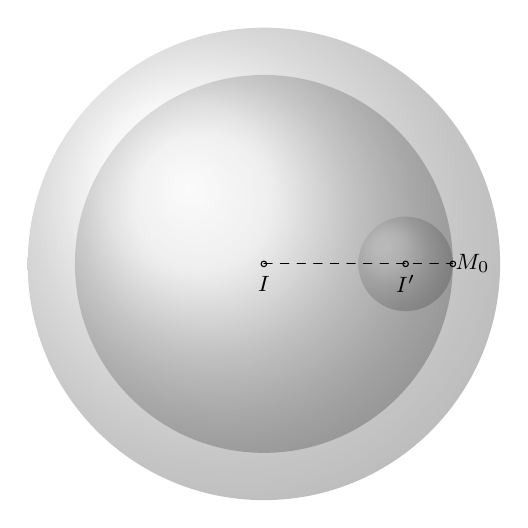
\begin{tikzpicture}[scale=1, font=\footnotesize, line join=round, line cap=round, >=stealth]
			% Định nghĩa tham số
			\def\rx{3}
			\def\ry{1/5*\rx}
			\def\rz{4/5*\rx}
			\def\rxx{3/5*\rx}
			% Điểm liên quan
			\coordinate (I) at (0,0);
			\coordinate (I') at (\rxx,0);
			\coordinate (M_0) at (\rz,0);
			%Vẽ 3 mặt cầu
			\shade[ball color = gray!20, opacity = 0.4] (I) circle (\rx cm);
			\shade[ball color = gray!40, opacity = 0.4] (I') circle (\ry cm);
			\shade[ball color = gray!30, opacity = 0.4] (I) circle (\rz cm);
			\draw[dashed] (I)--(I')--(M_0);
			\foreach \d/\g in {I/-90,I'/-90,M_0/0}
			\draw (\d) circle (1pt) node [shift={({\g}:0.25)}] {$\d$};
			\end{tikzpicture}}
		\noindent
		Gọi $M_0$ là tiếp điểm chung của $(S')$ và $(C)$, ta có $\overrightarrow{II'}=3\overrightarrow{I'M_0}\Leftrightarrow\heva{&x_0-1=\dfrac{1}{3}\\&y_0-2=\dfrac{2}{3}\\&z_0-3=\dfrac{2}{3}}\Leftrightarrow\heva{&x_0=\dfrac{4}{3}\\&y_0=\dfrac{8}{3}\\&z_0=\dfrac{11}{3}.}$\\
		Mặt phẳng $(P)$ qua $M_0\left(\dfrac{4}{3};\dfrac{8}{3};\dfrac{11}{3}\right)$ có véc-tơ pháp tuyến $\overrightarrow{II'}=(1;2;2)$. Phương trình của $(P)$ là
		$$x+2y+2z-14=0.$$
		Khoảng cách từ gốc tọa độ $O$ đến $(P)$ là $\mathrm{d}\left(O,(P)\right)=\dfrac{14}{3}$.\\
		$\bullet$ \textbf{Lưu ý:} \textit{Nếu $(C)$ và $(S')$ không tiếp xúc trong thì hoặc không tồn tại $(P)$ hoặc có vô số mặt phẳng $(P)$ thỏa mãn. Chính đề bài yêu cầu tính khoảng cách từ $(O)$ đến $(P)$ dẫn đến nhận định về tính duy nhất của $(P)$.}}
\end{ex}

\begin{ex}%[Thi thử, Thực hành Sư phạm - Đồng Nai, 2018]%[Đinh Thanh Hoàng, Dự án 12EX-11]%[2H3G2-7]
	Trong không gian với hệ trục tọa độ $Oxyz$ cho ba điểm $S(0; 0; 1)$, $M(m; 0; 0)$, $N(0; n; 0)$ với $m$, $n > 0$ và $m + n = 1$. Mặt phẳng $(SMN)$ luôn tiếp xúc với một mặt cầu cố định có bán kính là bao nhiêu biết mặt cầu đó đi qua điểm $A(1; 1; 1)$?
	\choice
	{$2$}
	{$\sqrt{2}$}
	{\True $1$}
	{$\sqrt{3}$}
	\loigiai{
		Phương trình mặt phẳng $(SMN)$ đi qua ba điểm $S(0; 0; 1)$, $M(m; 0; 0)$, $N(0; n; 0)$
		$$\dfrac{x}{m} + \dfrac{y}{n} + \dfrac{z}{1} = 1 \Leftrightarrow nx + my + mnz - mn = 0.$$
		Gọi $I$ là hình chiếu vuông góc của $A(1; 1; 1)$ trên mặt phẳng $(Oxy)$, ta có $I(1; 1; 0)$ và $IA = 1$.\\
		Ta có $\mathrm{d}\left(I, (SMN)\right) = \dfrac{|n + m - mn|}{\sqrt{m^2 + n^2 + m^2n^2}} = \dfrac{|1 - mn|}{\sqrt{(m + n)^2 - 2mn + m^2n^2}} = \dfrac{|1 - mn|}{\sqrt{(1 - mn)^2}} = 1$.\\
		Suy ra mặt phẳng $(SMN)$ luôn tiếp xúc với một mặt cầu tâm $I(1; 1; 0)$, bán kính $R = 1$.
	}
\end{ex}
\begin{dang}{Các bài toán cực trị}
	
\end{dang}
\setcounter{subsubsection}{0}
\setcounter{vd}{0}
\setcounter{bt}{0}
\setcounter{ex}{0}
\subsubsection{Ví dụ minh họa}
\begin{vd}%[2-GHK1-70, THPT Chuyên Lê Hồng Phong - Nam Định, 2018]%[Trần Xuân Thiện - Nguyễn Anh Tuấn, 12-EX-3-2019]%[2H3K2-8]
	Trong KG $Oxyz$, cho mặt phẳng $(P)\colon x+y-z+2=0$ và hai điểm $A(3;4;1)$, $B(7;-4;-3)$. Điểm $M(a;b;c)$, với $a>2$, thuộc mặt phẳng $(P)$ sao cho tam giác $ABM$ vuông tại $M$ và có diện tích nhỏ nhất. Tính giá trị biểu thức $a+b+c$.

	\loigiai{
		Ta có $S_{ABM}=\dfrac{1}{2}AB\cdot MH$ với $H$ là hình chiếu vuông góc của $M$ lên $AB$.\\
		Do $AB$ không đổi nên $\triangle ABM$ có diện tích nhỏ nhất khi $MH$ nhỏ nhất.\\ 
		Nhận thấy $\overrightarrow{AB}=(4;-8;-4)$, $\overrightarrow{n}_P=(1;1;-1)$ nên $\overrightarrow{AB}\cdot \overrightarrow{n}_P= 0$. Mà $A\notin (P)$, suy ra $AB \parallel (P)$.\\
		Do đó, $MH$ nhỏ nhất khi và chỉ khi $M$ thuộc giao tuyến của $(P)$ và $(Q)$, với $(Q)$ là mặt phẳng chứa $AB$ và vuông góc với $(P)$.
		Ta có $\overrightarrow{AB} \wedge \overrightarrow{n}_P=(12;0;12)$.	Suy ra mặt phẳng $(Q)$ đi qua $A$ và nhận $\overrightarrow{n}=(1;0;1)$ làm véc-tơ pháp tuyến có phương trình là $x+z-4=0$.\\
		Điểm $M$ nằm trên giao tuyến của $(P)$ và $(Q)$ nên có tọa độ thỏa mãn hệ phương trình $$\heva{&x+z-4=0\\ &x+y-z+2=0} \Rightarrow \heva{&x=t\\&y=2-2t\\&z=4-t} \Rightarrow M(t;2-2t;4-t), \ t>2.$$
		Ta có $\overrightarrow{AM}=(t-3;-2-2t;3-t)$ và $\overrightarrow{BM}=(t-7;6-2t;7-t)$.\\
		Tam giác $ABM$ vuông tại $M$ khi $$\overrightarrow{AM}\cdot \overrightarrow{BM}=0 \Leftrightarrow \hoac{&t=3\\ &t=\dfrac{5}{3}.}$$
		Vì $t>2$ nên chọn $t=3$ và lúc đó $M(3;-4;1)$, suy ra $a+b+c=0$.
	}
\end{vd}
\begin{vd}%[Thi thử lần 1, Lương Thế Vinh – Hà Nội -2018]%[Vũ Văn Trường, dự án(12EX-5)]%[2H3G2-8]
	Trong KG $Oxyz$, cho điểm $A\left(1;-6;1\right)$ và mặt phẳng $\left(P\right)\colon x+y+7=0$. Điểm $B$ thay đổi thuộc $Oz$; điểm $C$ thay đổi thuộc mặt phẳng $\left(P\right)$. Biết rằng tam giác $ABC$ có chu vi nhỏ nhất. Tìm tọa độ điểm $B$.
	\loigiai{
		\immini{Gọi $B_1$ là điểm đối xứng với $B$ qua $(P)$.\\
			$P_{ABC}=AB+BC+CA=AB+B_1C+CA\ge AB+AB_1$\\
			Gọi $M$ là hình chiếu của $A$ lên trục $Oz$, $M_1$ là điểm đối xứng của $M$ qua $(P)$\\
			$AB+AB_1\ge AM+AB_1\ge AM+AM_1$ (hằng số).\\
			Vậy $P_{ABC}$ nhỏ nhất khi $B\equiv M$ và $C$ là giao điểm của $AM_1$ với $(P)$.\\
			Từ đó suy ra tọa độ của điểm $B$ là $(0;0;1)$.}{
			\begin{tikzpicture}[scale=0.7]
			\clip (0,-4) rectangle(9.5,7.1);
			\tkzDefPoints{7/6/A,2/4/B,3/1/C,3/2/X,1/0/Y,7/0/Z,9/2/T,6/4/M,2/-3/B1,6/-3/M1, 1/4/D,8/4/W}
			\tkzDefMidPoint(B,B1) \tkzGetPoint{E}
			\tkzDefMidPoint(M,M1) \tkzGetPoint{F}
			\tkzInterLL(Y,Z)(B,B1) \tkzGetPoint{R}
			%\tkzInterLL(Y,Z)(C,B1) \tkzGetPoint{U}
			%\tkzInterLL(Y,Z)(A,B1) \tkzGetPoint{V}
			\tkzInterLL(Y,Z)(M,M1) \tkzGetPoint{S}
			\tkzInterLL(Y,Z)(A,M1) \tkzGetPoint{H}
			\tkzInterLL(X,T)(A,M1) \tkzGetPoint{J}
			\tkzInterLL(X,Y)(B,B1) \tkzGetPoint{I}
			\tkzDefBarycentricPoint(X=1,T=3) \tkzGetPoint{Q}
			\tkzDefBarycentricPoint(Y=1,Z=3) \tkzGetPoint{O}
			\tkzDefBarycentricPoint(Q=6,O=1) \tkzGetPoint{G}
			\tkzInterLL(O,Q)(A,M1) \tkzGetPoint{N}
			\tkzDrawSegments (I,Y Y,Z Z,T T,J Q,O D,W A,N  H,M1 A,B A,M E,F B,E R,B1 M,F S,M1 M1,B1 M,N)
			\tkzDrawSegments[dashed,thin](X,I X,J B,C A,C E,R F,S A,B1 C,B1 N,H)
			\tkzMarkRightAngle[think,size=0.3](B,M,A)
			\tkzMarkRightAngle[think,size=0.3](B1,M1,A)
			\tkzMarkAngle[think,size=0.8](X,T,Z)
			\tkzLabelAngle[dist=-0.5](Z,T,X){$P$}
			\tkzMarkSegments[thick,mark=|,color=blue](C,B C,B1)
			\tkzMarkSegments[thick,mark=||,color=blue](N,M N,M1)
			\tkzLabelPoints[above](A,B)
			\tkzLabelPoint[right](M1){$M_1$}
			\tkzLabelPoint[left](B1){$B_1$}
			\tkzLabelPoints[below right](M)
			\tkzLabelPoints[below right=-2pt](N)
			\tkzLabelPoints[below right=-2pt](C)
			\tkzDrawPoints[size=3](A,B,C,M,B1,M1,N,E,F)
			\end{tikzpicture}
		}
	}
\end{vd}
\begin{vd}%[DTH, Sở GD và ĐT - Hà Nam, 2019]%[Đào-V- Thủy, 12EX5]%[2H3K2-8]
	Trong không gian với hệ toạ độ $Oxyz$, cho $A(-3;0;0)$, $B(0;0;3)$, $C(0;-3;0)$ và mặt phẳng $(P)\colon x+y+z-3=0$. Tìm trên $(P)$ điểm $M$ sao cho $\left|\vec{MA}+\vec{MB}-\vec{MC}\right|$ nhỏ nhất.	
	\loigiai
	{Gọi $I(a;b;c)$ là điểm thoả mãn $\vec{MA}+\vec{MB}-\vec{MC}=\vec{0}$.\\
		Ta có $\vec{IA}=(-3-a;-b;-c)$, $\vec{IB}=(-a;-b;3-c)$, $\vec{IC}=(-a; 3-b; -c)$.\\
		$\vec{MA}+\vec{MB}-\vec{MC}=\vec{0}\Leftrightarrow \heva{&-3-a=0\\&b-3=0\\&3-c=0}\Leftrightarrow \heva{&a=-3\\&b=3\\&c=3}\Leftrightarrow I(-3;3;3)$.\\
		Nhận thấy $I(-3;3;3)\in (P)$. Ta có $\left|\vec{MA}+\vec{MB}-\vec{MC}\right|=\left|\vec{MI}+\vec{IA}+\vec{IB}-\vec{IC}\right|=MI\geq 0$.\\
		Từ đó suy ra $\left|\vec{MA}+\vec{MB}-\vec{MC}\right|$ nhỏ nhất bằng $0$ khi $M(-3;3;3)$.}
\end{vd}
\begin{vd}%[Đề tập huấn Sở Ninh Bình, 2019]%[Nguyễn Văn Hải, dự án(12EX-5-2019)]%[2H3G2-8]
	Trong KG $Oxyz$, cho hai mặt phẳng $(P) \colon x-y+z+3=0$, $(Q) \colon x+2y-2z-5=0$ và mặt cầu $(S) \colon x^2+y^2+z^2-2x+4y-6z-11=0$. Gọi $M$ là điểm di động trên $(S)$ và $N$ là điểm di động trên $(P)$ sao cho $MN$ luôn vuông góc với $(Q)$. Tìn giá trị lớn nhất của độ dài đoạn thẳng $MN$.

	\loigiai{ 
		\immini{Mặt cầu có tâm $I(1;-2;3)$ và bán kính $R=5$, $d(I,(P))=3\sqrt{3}, \mathrm{d}(I, (Q))=\dfrac{14}{3}$.\\
			Gọi $\alpha$ là góc giữa $(P)$ và $(Q)$.\\
			Khi đó $\cos \alpha=\dfrac{1}{\sqrt{3}}\Rightarrow \tan \alpha=\sqrt{2}$.\\
			Do đó $DK>NK=MI\Rightarrow CD \geq MN$.\\
			Ta có $\sin \alpha=\dfrac{IH}{IB}\Rightarrow IB=\dfrac{9}{\sqrt{2}}\Rightarrow BC=\dfrac{9+5\sqrt{2}}{\sqrt{2}}$.\\
			Mà $\tan \alpha=\dfrac{CD}{CB}\Rightarrow CD=BC\tan \alpha=9+5\sqrt{2}$. \\
			Vậy giá trị lớn nhất của độ dài đoạn $MN$ bằng $9+5\sqrt{2}$.
		}{
			\begin{tikzpicture}[scale=0.7, font=\footnotesize, line join=round, line cap=round, >=stealth]
			\tkzDefPoints{0/0/A, 5/0/a, 4/5/d,3/1/I,3/2.3/e}
			\tkzDrawCircle(I,e)
			\tkzDrawLine(A,d)
			\tkzDrawLine(A,a)
			\tkzDefLine[parallel=through I](A,a) \tkzGetPoint{c}
			\tkzInterLL(I,c)(A,d)\tkzGetPoint{B}
			\tkzDrawLine(B,I)
			\tkzDefPointBy[projection=onto A--a](I)
			\tkzGetPoint{i}
			\tkzDrawLine(i,I)
			\tkzInterLL(I,i)(A,d)\tkzGetPoint{N}
			\tkzInterLC(I,i)(I,e) \tkzGetSecondPoint{M}
			\tkzDefPointBy[projection=onto A--d](I) \tkzGetPoint{H}
			\tkzInterLC(I,B)(I,e) \tkzGetFirstPoint{C}
			\tkzDefLine[parallel=through C](M,I) \tkzGetPoint{b}
			\tkzInterLL(A,d)(C,b)\tkzGetPoint{D}
			\tkzDefPointBy[projection=onto C--D](N) \tkzGetPoint{K}
			\draw (B)--(C) (I)--(H)  (M)--(N)--(K) (C)--(D);
			\tkzDrawPoints(A,D,I,B,N,M,C,H,K) 
			\tkzLabelPoints[](A,I,M,C,K) 
			\tkzLabelPoints[above left](D,B,N,H) 
			\tkzMarkAngle(a,A,d) node[above right]{$\,\,\alpha$}
			\end{tikzpicture} 
		} 
	} 
\end{vd}
\begin{vd}%[Đề GHK2, Hàm Rồng, Thanh Hóa, năm 2019]%[Nguyễn Tiến Thùy, 12EX5-2019]%[2H3K2-8]
	Trong KG $Oxyz$, cho ba điểm $A(0;-2;-1)$, $B(-2;-4;3)$, $C(1;3;-1)$. Tìm điểm $M\in (Oxy)$ sao cho $\left|\overrightarrow{MA}+\overrightarrow{MB}+3\overrightarrow{MC}\right|$ đạt giá trị nhỏ nhất.
	\loigiai{
		Lấy điểm $I$ sao cho $\overrightarrow{IA}+\overrightarrow{IB}+3\overrightarrow{IC}=\vec{0}\Leftrightarrow\heva{&x_I=\dfrac{x_A+x_B+3x_c}{5}=\dfrac{1}{5}\\ &y_I=\dfrac{y_A+y_B+3y_c}{5}=\dfrac{3}{5}\\ &z_I=\dfrac{z_A+z_B+3z_c}{5}=-\dfrac{1}{5}}\Rightarrow I(\dfrac{1}{3};\dfrac{3}{5};-\dfrac{1}{5})$. 
		Khi đó ta có $\left|\overrightarrow{MA}+\overrightarrow{MB}+3\overrightarrow{MC}\right|=5\overrightarrow{MI}+\overrightarrow{IA}+\overrightarrow{IB}+3\overrightarrow{IC}=5\overrightarrow{MI}=5MI$.\\
		Từ đó, để $\left|\overrightarrow{MA}+\overrightarrow{MB}+3\overrightarrow{MC}\right|$ đạt giá trị nhỏ nhất, khi và chỉ khi $MI$ nhỏ nhất, điều đó xảy ra khi $M$ là hình chiếu của $I$ trên mặt phẳng $Oxy$, suy ra $M(\dfrac{1}{5};\dfrac{3}{5};0)$.
	}
\end{vd}
\subsubsection{Bài tập trắc nghiệm}
\begin{ex}%[Lê Quý Đôn, Hà Nội, lần 1, 2018]%[2H3G2-8]%[Nguyễn Bình Nguyên-12Ex7]
	Trong không gian với hệ trục tọa độ $Oxyz$, cho ba mặt phẳng $(P):x-2y+z-1=0, (Q):x-2y+z+8=0, (R):x-2y+z-4=0$. Một đường thẳng $d$ thay đổi cắt ba mặt phẳng $(P), (Q), (R)$ lần lượt tại $A, B, C$. Tìm giá trị nhỏ nhất của $T=AB^2+\dfrac{144}{AC}$.
	\choice
	{$72\sqrt[3]{3}$}
	{$96$}
	{\True $108$}
	{$72\sqrt[3]{4}$}
	\loigiai{
		\begin{center}
			\begin{tikzpicture}
			\tkzDefPoints{0/0/M, 5/0/N, 6/1.5/P, 1/1.5/Q}
			\tkzDrawPolygon(M,N,P,Q)
			\tkzDefPoints{0/2.5/A1, 5/2.5/B1, 6/3.5/C1, 1/3.5/D1}
			\tkzDrawPolygon(A1,B1,C1,D1)
			\tkzDefPoints{0/4/A2, 5/4/B2, 6/5.5/C2, 1/5.5/D2}
			\tkzDrawPolygon(A2,B2,C2,D2)
			\tkzMarkAngle[size=.65](N,M,Q)
			\draw (M) node[above right]{$Q$};
			\tkzMarkAngle[size=.65](B1,A1,D1)
			\draw (A1) node[above right]{$R$};
			\tkzMarkAngle[size=.65](B2,A2,D2)
			\draw (A2) node[above right]{$P$};
			\tkzDefPoints{1.5/1/B, 4/1/B', 4/5/A}
			\tkzInterLL(A2,B2)(A,B)
			\tkzGetPoint{I}
			\tkzInterLL(A2,B2)(A,B')
			\tkzGetPoint{J}
			\tkzInterLL(A1,B1)(A,B)
			\tkzGetPoint{H}
			\tkzInterLL(A1,B1)(A,B')
			\tkzGetPoint{K}
			
			
			\coordinate (C) at ($(B)!0.45!(A)$);
			\coordinate (C') at ($(B')!0.45!(A)$);
			\tkzInterLL(C1,D1)(A,C)
			\tkzGetPoint{I1}
			\tkzInterLL(C1,D1)(A,C')
			\tkzGetPoint{J1}
			\tkzDrawSegments[dashed](A,I A,J C,H C',K)
			\tkzDrawSegments(B,B' C,C' I,C J,C' H,B K,B')
			\tkzLabelPoints[left](B,C)
			\tkzLabelPoints[right](B',C')
			\tkzLabelPoints[above](A)
			\tkzMarkRightAngle(A,C',C)
			\tkzMarkRightAngle(A,B',B)
			\tkzDrawPoints(A, B, B', C, C')
			\end{tikzpicture}
		\end{center}
		Ta có $M(1;0;0)\in (P)$ và ba mặt phẳng $(P), (Q), (R)$ đôi một song song với nhau.\\
		Gọi $B', C'$ lần lượt là hình chiếu vuông góc của $A$ trên các mặt phẳng $(Q), (R)$.\\
		Ta có\\
		$AB'=d\left(A;(Q)\right)=d\left(M;(Q)\right)=\dfrac{|1-2.0+0+8|}{\sqrt{1^2+(-2)^2+1^2}}=\dfrac{3\sqrt{6}}{2}$.\\
		$AC'=d\left(A;(R)\right)=d\left(M;(R)\right)
		=\dfrac{|1-2.0+0-4|}{\sqrt{1^2+(-2)^2+1^2}}=\dfrac{\sqrt{6}}{2}$.\\
		Ta thấy $AB'=3AC'$ nên đặt $CC'=a\Rightarrow BB'=3a$.\\
		Ta có $AB^2=AB'^2+BB'^2=\dfrac{27}{2}+9a^2$; $AC=\sqrt{AC'^2+CC'^2}=\sqrt{\dfrac{3}{2}+a^2}$.\\
		$\begin{aligned} \Rightarrow 
		T=AB^2+\dfrac{144}{AC}=\dfrac{27}{2}+9a^2+\dfrac{144}{\sqrt{\dfrac{3}{2}+a^2}}
		&=9\left(\dfrac{3}{2}+a^2\right)+\dfrac{72}{\sqrt{\dfrac{3}{2}+a^2}}+\dfrac{72}{\sqrt{\dfrac{3}{2}+a^2}}\\
		&\geqslant 3\sqrt[3]{9\left(\dfrac{3}{2}+a^2\right).\dfrac{72}{\sqrt{\dfrac{3}{2}+a^2}}.\dfrac{72}{\sqrt{\dfrac{3}{2}+a^2}}}=108.
		\end{aligned}$.\\
		Do đó $\min T=108$ khi $a=\dfrac{\sqrt{2}}{2}$.
		
		
		
	}
\end{ex}
\begin{ex}%[Lê Quý Đôn, Hà Nội, lần 1, 2018]%[2H3G2-8]%[Phan Quốc Trí-12Ex7] 
	Trong không gian với hệ trục tọa độ $Oxyz$, cho điểm $M(1;1;1)$. Mặt phẳng $(P)$ qua $M$ cắt chiều dương của các trục $Ox,Oy, Oz$ lần lượt tại $A,B,C$ thõa mãn $OA=2OB$. Tính giá trị nhỏ nhất của thể tích khối chóp $OABC$.
	\choice
	{$\dfrac{64}{27}$}
	{$\dfrac{10}{3}$}
	{$\dfrac{9}{2}$}
	{\True $\dfrac{81}{16}$}
	\loigiai{
		Giả sử $A(a;0;0), B(0;b;0), C(0;0;c)$ với $a,b,c>0$. Khi đó mặt phẳng $(P)$ có dạng $\dfrac{x}{a}+\dfrac{y}{b}+\dfrac{z}{c}=1$. Vì $(P)$ đi qua $M$ nên $\dfrac{1}{a}+\dfrac{1}{b}+\dfrac{1}{c}=1$.\\
		Vì $OA=2OB \Rightarrow a=2b \Rightarrow \dfrac{3}{2b}+\dfrac{1}{c}=1 $.\\
		Thể tích khối tứ diện $OABC$ là $V=\dfrac{1}{6}abc=\dfrac{1}{3}b^2 c$.\\
		Ta có $1=\dfrac{3}{2b}+\dfrac{1}{c}=\dfrac{3}{4b}+\dfrac{3}{4b}+\dfrac{1}{c}\ge 3 \sqrt[3]{\dfrac{9}{16b^2c}} \Rightarrow \sqrt[3]{\dfrac{9}{16b^2c}} \le \dfrac{1}{3} \Rightarrow \dfrac{16b^2c}{9}\ge 27 \Rightarrow \dfrac{b^2c}{3}\ge \dfrac{81}{16}$.\\
		$V_{\min} = \dfrac{81}{16}$ khi $\dfrac{3}{4a}=\dfrac{1}{c}=\dfrac{1}{3}\Rightarrow \heva{&a=\dfrac{9}{2}\\& b=\dfrac{9}{4}\\&c=3}.$
	}
\end{ex}
\begin{ex}%[TT lần 2, Chuyên KHTN, Hà Nội 2018]%[2H3G2-8]%[Nguyện Ngô và Hồ Như Vương,12EX7]
	Trong không gian với hệ trục $Oxyz$, xét mặt cầu $(S)$ đi qua hai điểm $A(1; 6; 2),B(3; 0; 0)$ và có tâm thuộc mặt phẳng $(P): x-y+2=0$. Bán kính của mặt cầu $(S)$ có giá trị nhỏ nhất là
	\choice
	{\True $\dfrac{\sqrt{462}}{6}$}
	{$\dfrac{\sqrt{534}}{4}$}
	{ $\dfrac{\sqrt{218}}{6}$}
	{$\dfrac{\sqrt{530}}{4}$}
	\loigiai
	{
		Giả sử mặt cầu $(S)$ có tâm $I(x; y; z)$ và bán kính $R$. Ta có
		$$\begin{aligned}\heva{&IA^2=IB^2\\&I\in (P)}&\Leftrightarrow \heva{&(x-1)^2+(y-6)^2+(z-2)^2=(x-3)^2+y^2+z^2\\&x-y+2=0}\\
		&\Leftrightarrow\heva{&4x-12y-4z+32=0\\&x-y+2=0}\Leftrightarrow\heva{&z=2-2x\\&y=x+2.}
		\end{aligned}$$
		Khi đó
		$$R^2=IB^2=(x-3)^2+y^2+z^2=(x-3)^2+(x+2)^2+(2-2x)^2=6x^2-10x+17=6\left(x-\dfrac{5}{6}\right)^2+\dfrac{77}{6}.$$
		Suy ra $R\geq \sqrt{\dfrac{77}{6}}=\dfrac{\sqrt{462}}{6}$. Dấu bằng xảy ra khi $x=\dfrac{5}{6}$.	
	}
\end{ex}
\begin{ex}%[THPT Hương Khê-Hà Tĩnh năm 2017-2018-L1]%[2H3G2-8]%[Nguyễn Thế Út, 12EX-7]
	Trong KG $Oxyz$, biết mặt phẳng $(P)$ đi qua hai điểm $A(2;0;0)$, $M(1;1;1)$ đồng thời $(P)$ cắt các tia $Oy$, $Oz$ theo thứ tự tại hai điểm $B$, $C$ ($B$, $C$ đều không trùng với gốc tọa độ). Khi diện tích tam giác $ABC$ nhỏ nhất phương trình mặt phẳng $(P)$ là
	\choice
	{$y-z=0$}
	{$y+z-2=0$}
	{\True $2x+y+z-4=0$}
	{$x+y-2$}
	\loigiai{Ta thấy $(P)$ cắt trục $Ox$ tại điểm 
		$A(2;0;0)$. Gọi $B(0;b;0)$, $C(0;0;c)$ $(b, c \neq 0)$.\\
		Khi đó $(P): \dfrac{x}{2}+\dfrac{y}{b}+\dfrac{z}{c}=1$.
		
		$$M(1;1;1) \in (P)\Leftrightarrow \dfrac{1}{b}+\dfrac{1}{c}=\dfrac{1}{2}.$$
		Suy ra $\dfrac{1}{2} \geq \dfrac{2}{\sqrt{bc}} \Leftrightarrow bc \geq 16.$
		Ta có:	$\overrightarrow{AB}=(-2; b;0)$ , $\overrightarrow{AC}=(-2;0;c)$.
		
		$$S_{ABC}=\dfrac{1}{2}|[ \overrightarrow{AB}, \overrightarrow{AC}]|=\dfrac{1}{2}\sqrt{b^2c^2+4b^2+4c^2} \geq \dfrac{1}{2}\sqrt{b^2c^2+8bc} \geq \dfrac{1}{2} \sqrt{16^2+8 \cdot 16}.$$
		Dấu $"="$ xảy ra khi và chỉ khi $b=c=4$.\\
		Khi đó $(P): \dfrac{x}{2}+\dfrac{y}{4}+\dfrac{z}{4}=1$ hay $2x+y+z-4=0$.
	}
\end{ex}
\begin{ex}%[Đề KSCL HK1, trường chuyên Lê Hồng Phong, Nam Định, 2017 - 2018]%[2H3G2-8]%[Lê Đình Mẫn, 12EX-7]
	Trong không gian với hệ tọa độ ${Oxyz}$, cho hai điểm $M(0;-1;2)$ và $N(-1;1;3)$. Một mặt phẳng $(P)$ đi qua $M$, $N$ sao cho khoảng cách từ điểm $K(0;0;2)$. đến mặt phẳng $P$ đạt giá trị lớn nhất. Tìm tọa độ véc-tơ pháp tuyến $\overrightarrow{n}$ của mặt phẳng $(P)$.
	\choice
	{$\overrightarrow{n}=(1;-1;1)$}
	{\True $\overrightarrow{n}=(1;1;-1)$}
	{$\overrightarrow{n}=(2;-1;1)$}
	{$\overrightarrow{n}=(2;1;-1)$}
	\loigiai{\immini{Ta có: $\vec{MN}=(-1;2;1)$.\\
			Gọi $d$ là đường thẳng đi qua hai điểm $MN$.\\
			PTĐT $d$ đi qua $M(0;-1;2)$ và nhận $\vec{MN}=(-1;2;1)$ làm véc-tơ chỉ phương là: $\begin{cases}
			x=-1\\
			y=-1+2t\\
			z=2+t
			\end{cases}$.}{\begin{tikzpicture}[scale=1.0]
			\tkzDefPoints{0/0/A, -2/-2/B, 3/-2/C, 1/-0.5/M, 2.5/-1.5/N, 2.1/-0.3/E}
			\coordinate (D) at ($(A)+(C)-(B)$);
			\coordinate (H) at ($(M)!.3!(N)$);
			\coordinate (K) at ($(E)+(0,2)$);
			\tkzDrawLines(M,N)
			%\tkzDrawSegments[dashed](H,E)
			\tkzDrawSegments(K,E K,H H,E)
			\tkzDrawPolygon(A,B,C,D)
			\tkzLabelPoints[left](K,M,N,H)
			%\tkzLabelPoints[right](E)
			\tkzDrawPoints[fill=black](K,H,M,N,E)
			\tkzMarkRightAngle(K,H,M)
			\tkzMarkRightAngle(K,E,H)
			\tkzMarkAngle(C,B,A)
			\tkzLabelAngle[pos=0.7,rotate=40](C,B,A){$P$}
			\end{tikzpicture}}
		Gọi $H$ là hình chiếu của $K$ lên đường thẳng $d$.\\
		Ta có: $\mathrm{d}(K,(P))\leq KH$. Do đó $\mathrm{d}(K,(P))$ lớn nhất khi và chỉ khi $\mathrm{d}(K,(P))=KH$.\\
		Ta có $H\in d\Rightarrow H(-t;-1+2t;2+t)$;\\
		$\vec{KH}=(-t;-1+2t;t)$.\\
		Ta có: $KH\perp MN\Leftrightarrow \vec{KH}\cdot\vec{MN}=0\Leftrightarrow (-1)\cdot(-t)+2(-1+2t)+1\cdot t=0\Leftrightarrow t=\dfrac{1}{3}$.\\
		Lúc đó $\vec{KH}=\left(-\dfrac{1}{3};-\dfrac{1}{3};\dfrac{1}{3}\right)=-\dfrac{1}{3}\cdot\vec{n}$, với $\vec{n}=(1;1;-1)$.\\
		$\vec{KH}$ là véc-tơ pháp tuyến của mp$(P)$ nên $\vec{n}$ cũng là véc-tơ pháp tuyến của mp$(P)$.}
\end{ex}



\Closesolutionfile{ans}